\documentclass[12pt,a4paper]{report}

\usepackage{fontspec}
\usepackage{geometry}
\geometry{top=2.5cm,bottom=2.5cm,left=3cm,right=2.5cm}
\usepackage{setspace}
\onehalfspacing
\usepackage{graphicx}
\usepackage{float}
\usepackage{booktabs}
\usepackage{tabularx}
\usepackage{array}
\usepackage{xcolor}
\usepackage{tikz}
\usetikzlibrary{arrows.meta,positioning,shapes.geometric,shapes.multipart,fit,calc}
\usepackage{caption}
\usepackage{enumitem}
\usepackage{titlesec}
\usepackage{hyperref}
\usepackage{fancyhdr}
\usepackage{longtable}
\usepackage{pdflscape}
\usepackage{ragged2e}
\newcolumntype{L}[1]{>{\RaggedRight\arraybackslash}p{#1}}
\newcolumntype{Y}{>{\RaggedRight\arraybackslash}X}
\usepackage{polyglossia}
\setmainlanguage{french}
\setotherlanguage{english}
\setotherlanguage{arabic}
\setmainfont{TeX Gyre Termes}
\newfontfamily\arabicfont[Script=Arabic]{Amiri}

\definecolor{dxcblue}{RGB}{0,67,138}
\definecolor{dxcorange}{RGB}{255,105,0}
\definecolor{darkgray}{RGB}{55,65,81}
\definecolor{lightgray}{RGB}{243,244,246}
\definecolor{softblue}{RGB}{232,240,255}
\definecolor{covergreen}{RGB}{0,174,87}
\definecolor{coverburgundy}{RGB}{154,0,64}
\definecolor{covernavy}{RGB}{18,41,62}

\hypersetup{
    colorlinks=true,
    linkcolor=dxcblue,
    urlcolor=dxcblue,
    citecolor=dxcblue,
    pdftitle={Rapport PFE - Plateforme web d'evaluation de maturite},
    pdfauthor={Mahdi Mansour}
}

\captionsetup{font=small,labelfont=bf}
\setcounter{secnumdepth}{3}
\setcounter{tocdepth}{2}

\pagestyle{fancy}
\setlength{\headheight}{15pt}
\fancyhf{}
\fancyhead[L]{\leftmark}
\fancyhead[R]{Mahdi Mansour}
\fancyfoot[C]{\thepage}
\renewcommand{\headrulewidth}{0.4pt}

\titleformat{\chapter}[display]
{\normalfont\bfseries\color{dxcblue}}
{\chaptertitlename\ \thechapter}{12pt}{\Huge}
\titleformat{\section}
{\normalfont\large\bfseries\raggedright}
{\thesection}{1em}{}

\newcommand{\chapterintro}[1]{
    \vspace*{4cm}
    \begin{center}
        \begin{minipage}{0.78\textwidth}
            \centering
            \itshape «\,#1\,»
        \end{minipage}
    \end{center}
    \clearpage
}

\newcommand{\keyword}[1]{\textbf{#1}}

\begin{document}

\begin{titlepage}
    \thispagestyle{empty}
    \singlespacing
    \begin{tikzpicture}[remember picture, overlay]
        \fill[covergreen] ([xshift=1.35cm,yshift=-2.55cm]current page.north west) rectangle ++(0.35cm,-21.7cm);
        \fill[coverburgundy] ([xshift=1.35cm,yshift=1.35cm]current page.south west) rectangle ++(0.35cm,0.55cm);
    \end{tikzpicture}
    \centering
    \vspace*{0.9cm}
    \begin{minipage}{0.45\textwidth}
        \raggedright
        \hspace{0.9cm}
\includegraphics[width=5.4cm]{figures/emsi-logo.png}
    \end{minipage}
    \hfill
    \begin{minipage}{0.38\textwidth}
        \raggedleft
        
\includegraphics[width=3.9cm]{figures/dxc-logo.png}\hspace{0.5cm}
    \end{minipage}

    \vspace{2.0cm}
    {\Large\bfseries\color{covernavy} Rapport de stage de fin d'études}\\[0.45cm]
    {\Large\bfseries\color{covernavy} 5\textsuperscript{ème} année}\\[0.45cm]
    {\large\bfseries\color{covernavy} Filière : Ingénierie Informatique}\\[1.4cm]

    {\large\bfseries\color{covernavy} Sous le thème}\\[0.6cm]

    \hspace*{1.4cm}\rule{0.78\textwidth}{0.5pt}\\[0.55cm]
    \begin{minipage}{0.82\textwidth}
        \centering
        {\fontsize{22}{27}\selectfont\bfseries Conception et réalisation d'une plateforme web d'évaluation de la maturité Data Governance et AI Readiness}
    \end{minipage}\\[0.55cm]
    \hspace*{1.4cm}\rule{0.78\textwidth}{0.5pt}

    \vspace{0.9cm}
    {\large\bfseries Période de stage}\\[0.2cm]
    {\normalsize Du 16 février 2026 au 16 juin 2026}

    \vfill
    \begin{minipage}{0.42\textwidth}
        \raggedright
        \hspace{1.1cm}{\large\bfseries Réalisé par :}\\[0.25cm]
        \hspace{1.1cm}{\large Mahdi Mansour}\\[0.55cm]
        \hspace{1.1cm}{\normalsize Année universitaire : 2025--2026}
    \end{minipage}
    \hfill
    \begin{minipage}{0.52\textwidth}
        \raggedright
        {\large\bfseries Encadré par :}\\[0.25cm]
        {\large Dr. Omar EL Midaoui}\\
        {\normalsize\itshape EMSI}\\[0.18cm]
        {\large Mme. Meriyem Habbar}\\
        {\normalsize\itshape Encadrante d'entreprise, DXC Technology}\\[0.18cm]
        {\large Mr. Younes Elgargouh}\\
        {\normalsize\itshape Encadrement opérationnel, DXC Technology}\\[0.35cm]
        {\large\bfseries Entreprise : DXC Technology}
    \end{minipage}
    \vspace*{0.6cm}
\end{titlepage}
\onehalfspacing

\pagenumbering{roman}
\chapter*{Dédicaces}
\markboth{Dédicaces}{}
\addcontentsline{toc}{chapter}{Dédicaces}
Je dédie ce modeste travail à mes parents, dont la confiance et les efforts silencieux ont accompagné chaque étape de mon parcours. Ce qu'ils m'ont transmis, bien au-delà des études, reste la part la plus précieuse de cette réussite.

Je le dédie également à ma famille, dont la présence discrète mais constante m'a offert l'équilibre nécessaire pour avancer sereinement, ainsi qu'à mes amis, qui ont rendu ces années de formation plus humaines par leur écoute et leur soutien.

Je l'adresse enfin à mes enseignants et à mes encadrants, dont les remarques, parfois exigeantes, m'ont aidé à structurer ma réflexion et à affiner mon regard professionnel. Qu'ils trouvent dans ces pages l'expression sincère de ma reconnaissance.

\chapter*{Remerciements}
\markboth{Remerciements}{}
\addcontentsline{toc}{chapter}{Remerciements}
Au terme de ce stage de fin d'études, je tiens à exprimer ma reconnaissance à toutes les personnes qui ont contribué, par leur disponibilité et leurs conseils, au bon déroulement de ce travail.

Je remercie tout d'abord mon encadrant académique, Monsieur Omar EL Midaoui, pour son suivi rigoureux et ses remarques constructives. Son accompagnement m'a aidé à structurer ma démarche et à inscrire la réflexion dans un cadre académique cohérent.

Mes remerciements s'adressent à Madame Meriyem Habbar, mon encadrante d'entreprise au sein de DXC Technology, pour la confiance qu'elle m'a accordée durant ce stage et pour le cadre qu'elle a su mettre en place autour de notre projet.

J'adresse également un remerciement particulier à Monsieur Younes Elgargouh, qui a assuré l'encadrement opérationnel au quotidien. Sa disponibilité, ses orientations techniques et ses retours réguliers m'ont permis de mieux saisir les enjeux métier d'une plateforme destinée à un usage de conseil et d'avancer dans de bonnes conditions tout au long du projet.

Je tiens également à remercier DXC Technology pour l'opportunité d'évoluer dans un environnement professionnel exigeant, autour d'un sujet à la croisée de la gouvernance des données et de l'intelligence artificielle. Cette expérience m'a permis de confronter mes acquis aux contraintes concrètes d'un projet d'entreprise.

J'exprime aussi ma gratitude à l'École Marocaine des Sciences de l'Ingénieur, à son corps professoral et à son personnel administratif, pour la qualité de la formation dispensée durant ces années d'études.

Je remercie également Hiba Bouhnin, qui a réalisé le module Agent IA dans le cadre du même projet, pour la collaboration et les échanges autour de son intégration dans la plateforme, ainsi que Saad Khalmadani, ingénieur DevOps chez DXC Technology, qui s'est greffé au projet pour porter la solution en production sur Azure et m'a permis de voir l'aboutissement du travail dans un environnement réel.

Mes remerciements vont enfin aux membres du jury pour l'attention qu'ils porteront à ce travail.

\chapter*{Résumé}
\markboth{Résumé}{}
\addcontentsline{toc}{chapter}{Résumé}
Ce projet de fin d'études porte sur la conception et la réalisation d'une plateforme web destinée à l'évaluation de la maturité des organisations en matière de Data Governance et d'AI Readiness. Le besoin, exprimé par DXC Technology, vient du constat que les évaluations reposaient sur des supports dispersés, peu adaptés à un suivi homogène entre consultants, clients et campagnes successives. La problématique consistait alors à proposer un environnement unifié, multilingue et sécurisé, permettant de préparer les questionnaires, gérer les invitations, collecter les réponses et exploiter les résultats.

La solution adoptée repose sur une architecture full-stack conteneurisée associant un frontend Next.js, un backend Spring Boot, une base PostgreSQL, une authentification fédérée via Keycloak et un service d'Agent IA exposé en FastAPI. Le développement a suivi une démarche agile et incrémentale, structurée autour de quatre versions livrées entre février et juin 2026~: V1 livre la plateforme initiale (multi-domaine, multilingue, administration et analytique), V2 intègre l'Agent IA dans les flux métier, V3 ajoute le copilote « Build with AI » et prépare le déploiement en production, V4 finalise la couverture multilingue de l'IA et l'édition des brouillons. Ma contribution personnelle concerne l'ensemble de la plateforme applicative, à l'exception du module Agent IA, réalisé par Hiba Bouhnin.

La version livrée couvre le cycle complet d'une évaluation, de la préparation du questionnaire à l'exploitation analytique des soumissions, tout en conservant une validation humaine sur les recommandations produites par l'Agent IA.

\textbf{Mots-clés :} Data Governance, AI Readiness, Next.js, Spring Boot, Évaluation de maturité.

\chapter*{Abstract}
\markboth{Abstract}{}
\addcontentsline{toc}{chapter}{Abstract}
\begin{english}
This graduation project addresses the design and implementation of a web platform dedicated to assessing organizational maturity in Data Governance and AI Readiness. The need, raised by DXC Technology, came from the observation that assessments relied on scattered documents poorly suited to a consistent follow-up across consultants, clients and successive campaigns. The challenge was therefore to provide a unified, multilingual and secure environment supporting questionnaire authoring, invitation management, answer collection and result analysis.

The chosen solution relies on a containerized full-stack architecture combining a Next.js frontend, a Spring Boot backend, a PostgreSQL database, federated authentication through Keycloak, and an AI Agent service exposed via FastAPI. Development followed an agile, incremental approach organized in four successive versions delivered between February and June 2026~: V1 delivers the initial platform (multi-domain, multilingual, administration and analytics), V2 integrates the AI Agent into the business flows, V3 adds the “Build with AI” copilot and prepares production deployment, and V4 finalises the AI's multilingual coverage and the editing of drafts. My personal contribution concerns the entire application platform, with the exception of the AI Agent module, developed by Hiba Bouhnin.

The delivered version covers the full assessment cycle, from questionnaire preparation to the analytical exploitation of submissions, while keeping a human validation layer on the recommendations produced by the AI Agent.
\end{english}

\textbf{Keywords:} Data Governance, AI Readiness, Next.js, Spring Boot, Maturity Assessment.

\tableofcontents
\listoffigures
\listoftables

\chapter*{Liste des abréviations}
\markboth{Liste des abréviations}{}
\addcontentsline{toc}{chapter}{Liste des abréviations}
\begin{longtable}{>{\bfseries}L{3cm}L{11cm}}
API & Application Programming Interface \\
BPO & Business Process Outsourcing \\
CDG & Caisse de Dépôt et de Gestion \\
CI/CD & Continuous Integration / Continuous Deployment \\
CODIR & Comité de Direction \\
CRUD & Create, Read, Update, Delete \\
CSV & Comma-Separated Values \\
DTO & Data Transfer Object \\
EMSI & École Marocaine des Sciences de l'Ingénieur \\
HTTPS & HyperText Transfer Protocol Secure \\
IA & Intelligence Artificielle \\
IdP & Identity Provider \\
ITO & Infrastructure Technology Outsourcing \\
JPA & Java Persistence API \\
JPQL & Java Persistence Query Language \\
JSON & JavaScript Object Notation \\
JSONB & JavaScript Object Notation -- Binary (PostgreSQL) \\
JWKS & JSON Web Key Set \\
JWT & JSON Web Token \\
LLM & Large Language Model \\
OAuth2 & Open Authorization (version 2) \\
OIDC & OpenID Connect \\
ORM & Object-Relational Mapping \\
PDF & Portable Document Format \\
PFE & Projet de Fin d'Études \\
PKCE & Proof Key for Code Exchange \\
REST & Representational State Transfer \\
ROPC & Resource Owner Password Credentials \\
RTL & Right-To-Left \\
SMTP & Simple Mail Transfer Protocol \\
SPA & Single Page Application \\
SQL & Structured Query Language \\
SSO & Single Sign-On \\
TLS & Transport Layer Security \\
UML & Unified Modeling Language \\
UUID & Universally Unique Identifier \\
\end{longtable}

\cleardoublepage
\pagenumbering{arabic}

\chapter*{Introduction générale}
\markboth{Introduction générale}{}
\addcontentsline{toc}{chapter}{Introduction générale}
La donnée occupe aujourd'hui une place centrale dans la prise de décision, les opérations et les projets d'innovation des entreprises. L'essor de l'intelligence artificielle accentue cette tendance, mais exige en retour un niveau de maturité minimal en matière de gouvernance, de qualité, de sécurité et d'exploitation des données. Avant d'engager des initiatives d'envergure, les organisations doivent donc pouvoir évaluer leur propre capacité à structurer et à valoriser leurs données.

C'est le type de diagnostic que DXC Technology propose à ses clients, à travers des évaluations de maturité portant sur la Data Governance et l'AI Readiness. Lorsque ces évaluations reposent sur des fichiers dispersés et des échanges manuels, leur préparation et leur exploitation deviennent vite coûteuses~: les questionnaires évoluent, les réponses doivent être consolidées, les invitations doivent être suivies et les résultats doivent finalement être restitués sous une forme exploitable par le consultant et son client.

Le présent projet répond à ce besoin par la conception et la réalisation d'une plateforme web destinée à centraliser l'ensemble de cette démarche~: administration du référentiel, suivi des invitations, collecte des réponses, calcul des scores de maturité, restitution analytique et production assistée de rapports. Une attention particulière a été portée à l'accessibilité linguistique (français, anglais et arabe avec adaptation RTL) et à la sécurité d'accès, avec un module d'Agent IA chargé d'enrichir l'analyse sans se substituer au jugement du consultant. Le travail a été conduit selon une démarche agile et incrémentale~: quatre versions livrées entre février et juin 2026, chacune apportant un palier fonctionnel vérifiable. Ma contribution couvre la totalité de la plateforme applicative, à l'exception du module Agent IA développé en parallèle par Hiba Bouhnin et présenté ici sous l'angle de son intégration.

Le présent rapport s'articule autour de cinq chapitres principaux~:

{\color{dxcblue}\textbf{Le premier chapitre}} présente l'organisme d'accueil et situe le contexte du projet. Il décrit DXC Technology et sa filiale marocaine, formule la problématique adressée et expose la solution envisagée ainsi que son apport métier.

{\color{dxcblue}\textbf{Le deuxième chapitre}} aborde la méthodologie de travail et la gestion du projet. Il détaille l'équipe, le découpage en quatre versions contractuelles, les critères de validation, la planification et les pratiques d'assurance qualité retenues.

{\color{dxcblue}\textbf{Le troisième chapitre}} se concentre sur l'analyse des besoins et la conception. Il formalise les besoins fonctionnels et non fonctionnels, identifie les acteurs et les règles métier, puis présente les diagrammes UML (cas d'utilisation, classes, séquence) qui sous-tendent le système.

{\color{dxcblue}\textbf{Le quatrième chapitre}} traite de l'étude technique. Il décrit l'architecture multi-services adoptée, justifie le choix de chaque technologie (Next.js, Spring Boot, Keycloak, PostgreSQL, FastAPI, Docker), et explique les choix d'intégration continue et de mise en production.

{\color{dxcblue}\textbf{Enfin, le cinquième chapitre}} restitue la réalisation au fil des quatre versions livrées. Il présente le périmètre, les choix d'implémentation et les livrables de chaque version, illustrés par des captures d'écran de la plateforme et par les résultats des tests automatisés.

Le rapport se termine par une conclusion générale, une discussion des limites de la solution et des perspectives d'évolution.

\chapter{Contexte général du projet}
\chapterintro{Ce chapitre situe le projet dans son contexte~: l'entreprise d'accueil, l'usage métier auquel la plateforme répond et la problématique à laquelle elle cherche à apporter une réponse.}

\section{Présentation de l'organisme d'accueil}
DXC Technology est une entreprise internationale de services informatiques née en avril 2017 de la fusion entre CSC, acteur historique du conseil en systèmes d'information, et HP Enterprise Services, leader des services IT issus du groupe Hewlett-Packard \cite{dxcorg}. Avec un chiffre d'affaires annuel de l'ordre de 25 milliards de dollars et un portefeuille d'environ 6\,000 clients répartis dans plus de 70 pays, l'entreprise occupe une position importante dans le secteur de la transformation digitale.

Les offres de DXC sont organisées autour de deux grandes lignes de service. La première, dite \textit{Global Business Services} (GBS), regroupe les solutions logicielles et les prestations destinées à accompagner les organisations dans leur transformation digitale et l'optimisation de leurs processus métier~: conseil, analytique, ingénierie logicielle et solutions industrielles. La seconde, \textit{Global Infrastructure Services} (GIS), prend en charge le cloud, les plateformes, la mobilité, l'Internet des objets et la cybersécurité \cite{dxcorg}. Cette répartition explique le positionnement transversal de l'entreprise, simultanément intégrateur, conseil et opérateur de services.

L'activité de DXC s'appuie également sur un écosystème étendu de partenaires technologiques (Amazon Web Services, Microsoft, Oracle, SAP, Red Hat, ServiceNow, VMware, Dell Technologies, IBM, Salesforce, etc.) qui contribuent à étendre la portée des solutions proposées et à raccourcir les délais de mise en œuvre chez les clients.

\section{DXC Technology Maroc}
DXC Technology Maroc, héritière de HP CDG IT Services Maroc implantée depuis 2007, est une co-entreprise détenue à 51\,\% par DXC Technology et à 49\,\% par le Groupe CDG, premier investisseur institutionnel du Royaume \cite{dxcorg}. L'entité regroupe plus de 1\,500 collaborateurs sur trois sites de production~: Technopolis (Rabat--Salé), Hay Riad (Rabat) et Casa Near Shore (Casablanca). Elle accompagne des donneurs d'ordre publics et privés, marocains et internationaux, dans leur transformation digitale en apportant son expertise en conseil, en solutions logicielles et en services technologiques.

Les métiers de DXC Maroc couvrent cinq grands domaines~: \textit{Cloud \& Infrastructure} pour la modernisation des environnements hybrides, \textit{Data Center} pour l'hébergement et le pilotage des infrastructures, \textit{Cyber Security} pour la supervision, la détection et la réponse aux incidents, \textit{BI \& Analytics} pour les solutions décisionnelles et de visualisation des données, et enfin \textit{Business Process} pour l'optimisation des processus métier et l'intégration de techniques d'intelligence artificielle \cite{dxcorg}. Cette dernière brique recoupe directement le présent projet, qui se situe à l'intersection de la donnée, de l'évaluation de maturité et de l'IA.

Côté prestations, DXC Maroc opère principalement sur quatre lignes~: gestion des infrastructures (ITO, \textit{Infrastructure Technology Outsourcing}), gestion du poste de travail et des processus métier (BPO et \textit{Global Service Desk}), gestion des applications et assurance logicielle (APPS), et l'analyse, l'ingénierie et la sécurité \cite{dxcorg}. Dans le cadre de ce stage, DXC Technology joue le rôle d'organisme d'accueil et de cadre métier~: la plateforme développée vise à outiller les consultants dans la conduite d'évaluations de maturité Data Governance et AI Readiness auprès de leurs clients.

\begin{table}[H]
\centering
\caption{Chiffres clés et repères de DXC Technology et de sa filiale marocaine.}
\begin{tabularx}{\textwidth}{>{\bfseries}L{4.5cm}Y}
\toprule
Indicateur & Valeur \\
\midrule
Création de DXC Technology & Avril 2017 (fusion CSC + HP Enterprise Services) \\
Chiffre d'affaires annuel & Environ 25 milliards de dollars \\
Portefeuille clients & ${\sim}6\,000$ clients dans plus de 70 pays \\
Lignes de service mondiales & Global Business Services et Global Infrastructure Services \\
Implantation au Maroc & Depuis 2007 (ex-HP CDG IT Services Maroc) \\
Structure capitalistique au Maroc & Joint-venture DXC (51\,\%) -- Groupe CDG (49\,\%) \\
Effectif au Maroc & Plus de 1\,500 collaborateurs \\
Sites de production & Technopolis, Hay Riad, Casa Near Shore \\
\bottomrule
\end{tabularx}
\label{tab:dxc-chiffres}
\end{table}

\begin{table}[H]
\centering
\caption{Domaines d'activité DXC Technology Maroc en lien avec le projet.}
\begin{tabularx}{\textwidth}{>{\bfseries}L{4cm}Y}
\toprule
Domaine & Lien avec le projet \\
\midrule
BI et analyse de données & Exploitation des résultats d'évaluations, tableaux de bord et indicateurs de maturité. \\
Cybersécurité & Extension possible des évaluations vers la résilience cybersécurité et la gouvernance des risques. \\
Cloud et Infrastructure & Contexte de transformation digitale et de modernisation des environnements clients. \\
Processus métiers & Standardisation des processus d'évaluation, de suivi et de reporting. \\
Data & Évaluation de la gouvernance, de la qualité et de l'exploitation des données. \\
\bottomrule
\end{tabularx}
\end{table}

\section{Organisation interne de DXC Maroc}
L'entité marocaine est dirigée par un \textit{Center Lead} qui anime un comité de direction (CODIR) couvrant l'ensemble des fonctions opérationnelles et de support. La figure~\ref{fig:organigramme-dxc} reproduit l'organigramme officiel issu du document de présentation de l'organisme d'accueil \cite{dxcorg}. Il fait apparaître, sous l'autorité du \textit{Center Lead}, sept directions principales (Audit \& Risque, \textit{Project \& Run Lead}, \textit{Manage Lead}, \textit{Business Operations}, Finance, Ressources Humaines, \textit{New Business}), ainsi que les responsables des entités opérationnelles (ABS, ITO, GOC, WPS), des secteurs (Manufacturing \& Distribution, Health and Life Sciences, Financial Services, Public Sector, Education) et des fonctions support (communication, juridique, IT, sécurité, finance, RH).

\begin{figure}[H]
\centering
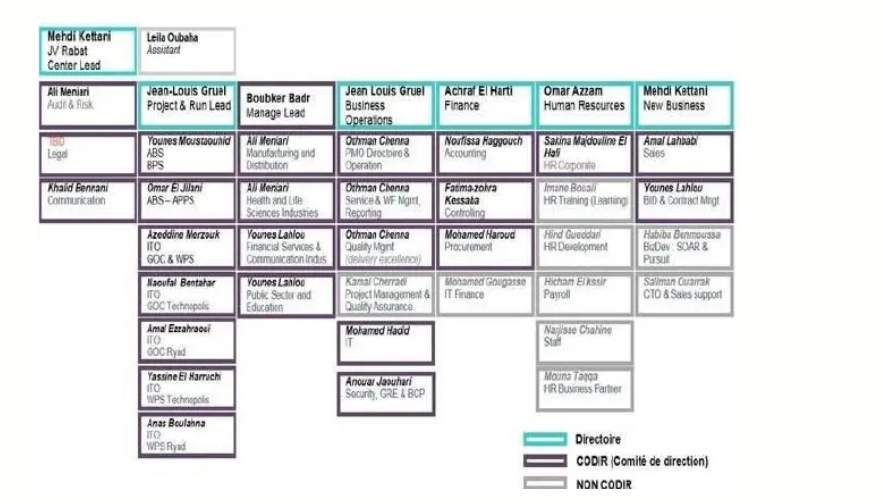
\includegraphics[width=\textwidth]{figures/dxc-organigramme.png}
\caption[Organigramme de DXC Technology Maroc]{Organigramme officiel de DXC Technology Maroc, distinguant visuellement le Directoire (cadre vert), les membres du comité de direction (cadre bordeaux) et les responsables hors CODIR. Source~: document interne de présentation de l'organisme d'accueil \cite{dxcorg}.}
\label{fig:organigramme-dxc}
\end{figure}

\section{Contexte du projet}
Les évaluations de maturité servent à identifier les points forts, les faiblesses et les priorités d'amélioration d'une organisation. Pour les consultants, elles donnent un cadre de diagnostic et aident à comparer les résultats entre domaines avant de préparer des recommandations.

Avant la mise en place de la plateforme, ce type d'évaluation pouvait être réalisé à l'aide de documents, de fichiers de suivi ou de formulaires non intégrés. Ce mode de fonctionnement reste acceptable pour un faible volume, mais il devient plus lourd lorsque le nombre de clients, de domaines et de réponses augmente. Les limites principales sont le manque de standardisation, la consolidation manuelle des réponses, l'absence de visualisation immédiate des résultats et le suivi manuel des invitations.

\section{Étude de l'existant}
L'existant fonctionnel peut être résumé par un processus d'évaluation dépendant de supports séparés. Les questions, les réponses, les relances clients et les analyses sont traitées dans des outils différents. Cette séparation augmente le risque d'erreur, rend le suivi d'une évaluation moins fluide et limite la réutilisation des données.

\begin{table}[H]
\centering
\caption{Comparaison entre le fonctionnement initial et la solution proposée pour le processus d'évaluation.}
\small
\begin{tabularx}{\textwidth}{>{\bfseries}L{3.5cm}Y Y}
\toprule
Critère & Fonctionnement initial & Solution proposée \\
\midrule
Collecte des réponses & Formulaires ou fichiers séparés, consolidation manuelle. & Parcours web centralisé avec soumission structurée. \\
Suivi client & Relances et statuts suivis manuellement. & Invitations avec statut, expiration et renvoi. \\
Analyse & Calculs dispersés et visualisation limitée. & Scores automatiques, heatmaps, graphiques et exports. \\
Adaptation linguistique & Gestion difficile des versions multilingues. & Interfaces et contenus français, anglais et arabe. \\
Rapports & Rédaction majoritairement manuelle. & Brouillons et rapports assistés par Agent IA. \\
\bottomrule
\end{tabularx}
\label{tab:existant}
\end{table}

\section{Problématique}
La problématique principale peut être formulée ainsi :

\begin{quote}
Comment concevoir une application web sécurisée et multilingue capable de préparer les évaluations Data Governance et AI Readiness, de collecter les réponses, d'analyser les résultats et d'aider les consultants à produire des rapports utilisables ?
\end{quote}

Cette problématique fait apparaître plusieurs enjeux. Les administrateurs doivent pouvoir faire évoluer les questionnaires sans intervention directe dans le code. Les clients doivent disposer d'un parcours clair, accessible et adapté à leur langue. Les consultants doivent, de leur côté, accéder rapidement aux résultats, comparer les scores et préparer des rapports sans refaire les calculs manuellement.

\begin{table}[H]
\centering
\caption{Enjeux principaux associés à la digitalisation du processus d'évaluation.}
\begin{tabularx}{\textwidth}{>{\bfseries}L{3.5cm}Y}
\toprule
Enjeu & Description \\
\midrule
Standardisation & Uniformiser la structure des questionnaires et limiter les variations entre évaluations. \\
Traçabilité & Conserver les invitations, les réponses, les scores et les rapports associés aux clients. \\
Analyse & Transformer les réponses collectées en indicateurs lisibles pour les consultants. \\
Multilingue & Proposer un parcours adapté au français, à l'anglais et à l'arabe, y compris pour l'affichage RTL. \\
Assistance & Fournir une aide à la rédaction des recommandations tout en gardant une validation humaine. \\
\bottomrule
\end{tabularx}
\end{table}

\section{Objectifs du projet}
Les objectifs retenus couvrent le parcours d'évaluation complet. La plateforme devait proposer les évaluations Data Governance et AI Readiness, gérer les sections, les questions et les choix depuis un espace administrateur, puis collecter les réponses et calculer les scores de maturité. Elle devait aussi prendre en charge les invitations internes ou externes, afficher les résultats dans des tableaux de bord, intégrer le module IA pour les recommandations et les rapports, et rester utilisable en français, anglais et arabe avec support RTL. Les espaces réservés aux administrateurs devaient enfin être protégés par authentification et contrôle des rôles.

\section{Périmètre du projet}
Le périmètre du projet couvre le cycle d'évaluation, depuis la préparation du questionnaire jusqu'à l'analyse des résultats. Il inclut les évaluations Data Governance et AI Readiness, la gestion des domaines clients, les invitations, les soumissions, les tableaux de bord et l'intégration du module IA. Le type Cybersecurity Resilience apparaît également dans certaines interfaces de démonstration, car la structure technique de la plateforme permet d'ajouter plusieurs familles d'évaluations.

Le projet ne vise pas à remplacer le travail d'expertise du consultant. Il fournit un support numérique pour fiabiliser la collecte, accélérer l'analyse et produire une première base de recommandations. La validation finale des conclusions reste une responsabilité humaine.

Le périmètre personnel présenté dans ce rapport concerne la plateforme applicative, de l'interface jusqu'aux services backend et à l'intégration de l'authentification. Les aspects liés à l'Agent IA sont décrits lorsqu'ils interviennent dans l'expérience utilisateur ou dans l'intégration avec les écrans réalisés.

\section{Solution proposée}
La réponse retenue prend la forme d'une plateforme full-stack qui réunit cinq briques complémentaires~: un frontend Next.js pour les parcours et l'interface d'administration, un backend Spring Boot pour exposer les services métier, une base PostgreSQL pour la persistance, un serveur Keycloak pour l'authentification fédérée, et un service Agent IA en FastAPI pour les fonctions analytiques avancées. Chacune de ces briques est conteneurisée afin de faciliter le déploiement et la reproductibilité de l'environnement.

La plateforme n'a pas été conçue comme un formulaire figé. Les types d'évaluation, les sections, les questions, les choix et certains éléments visuels (logos, intitulés) sont stockés en base comme des données applicatives. Les consultants peuvent ainsi faire évoluer un questionnaire ou en introduire un nouveau sans toucher au code source, ce qui est essentiel pour un outil destiné à durer plusieurs campagnes d'évaluation.

\begin{figure}[H]
\centering
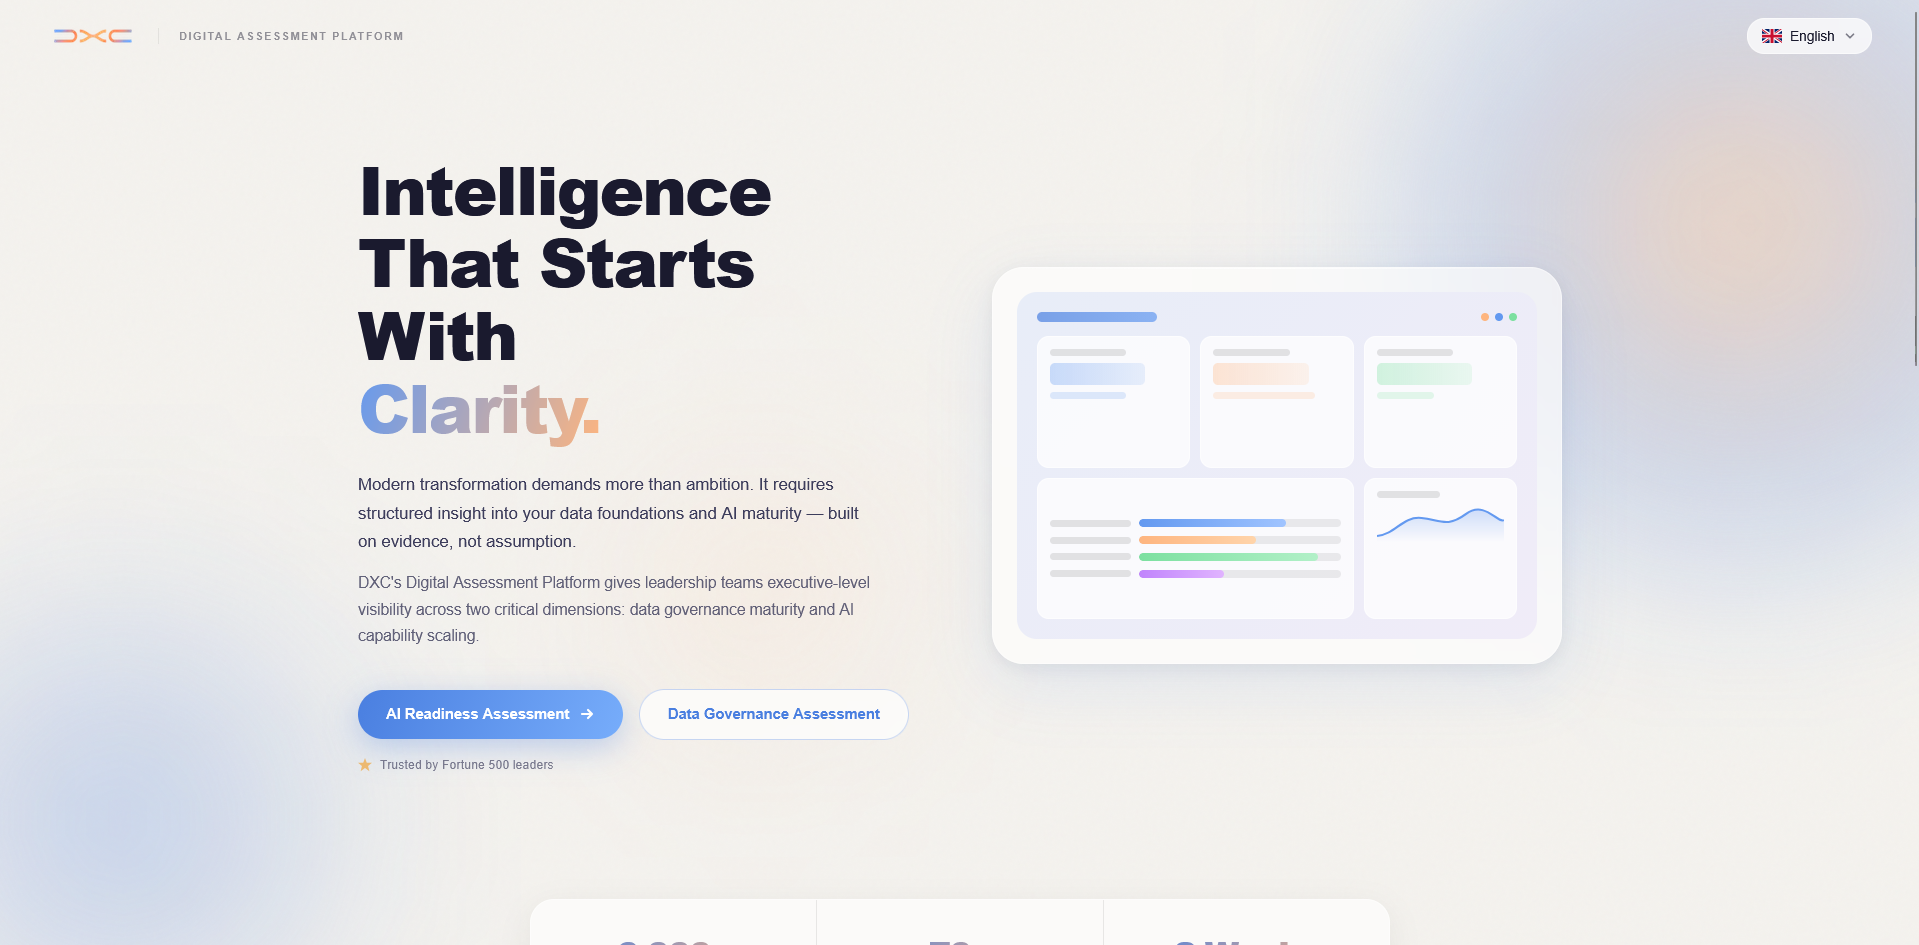
\includegraphics[width=0.95\textwidth]{figures/homepage.png}
\caption[Page d'accueil de la plateforme]{Page d'accueil de la plateforme Digital Assessment Platform, présentant l'accès aux parcours d'évaluation AI Readiness et Data Governance ainsi que le sélecteur de langue.}
\label{fig:preview}
\end{figure}

La figure \ref{fig:preview} montre la page d'accueil, avec l'accès direct aux parcours d'évaluation et au choix de langue.

\section{Apport de la solution}
L'apport de la plateforme tient d'abord à un effet de regroupement. Ce qui s'effectuait auparavant à travers plusieurs supports (préparation des questionnaires dans un document, suivi des invitations par courriel, consolidation des réponses dans un tableur, restitution dans une présentation) se fait désormais dans un environnement unique, avec une traçabilité homogène. Cette centralisation réduit les manipulations manuelles, fiabilise les données collectées et libère du temps que les consultants peuvent réinvestir dans l'analyse.

Côté usage quotidien, la combinaison des tableaux de bord, des filtres, des vues détaillées et des exports CSV change la nature du travail. Le consultant passe en quelques clics d'une vue globale de son portefeuille clients à l'analyse fine d'une soumission individuelle. Les écrans analytiques ont demandé plusieurs itérations~: ils restent fonctionnels sur un cas minimal, mais il fallait s'assurer que la lecture reste exploitable lorsque le volume de clients, de domaines ou de réponses augmente.


\section{Conclusion}
Ce chapitre a posé le cadre du projet~: l'organisme d'accueil, l'usage métier visé, la problématique et la solution envisagée. La suite du rapport décrit la manière dont ce projet a été conduit, puis présente la conception et la réalisation de la plateforme.

\chapter{Plan qualité projet}
\chapterintro{Construire une plateforme métier en quelques mois suppose une organisation explicite. Ce chapitre revient sur la manière dont le projet a été conduit~: la méthodologie agile retenue, la composition de l'équipe, la planification des quatre versions successives, ainsi que les pratiques de qualité et de gestion des risques qui ont accompagné la réalisation.}

\section{Méthodologie de travail}
Le projet a été conduit selon une approche agile incrémentale, structurée en quatre versions contractuelles successives (V1 à V4). Chacune regroupe un lot cohérent de fonctionnalités, livré à une date précise et présenté à l'encadrement avant le démarrage de la suivante. Ce découpage rend l'avancement visible, fixe des points de validation clairs et autorise une révision des priorités d'une version à l'autre selon les retours reçus.

Cette méthode convenait au contexte du projet, où certains besoins se sont précisés au fur et à mesure de la réalisation. Les écrans analytiques et l'espace d'administration ont demandé plusieurs itérations~; l'intégration entre la plateforme et l'Agent IA, développé en parallèle, devait être validée par étapes pour éviter les blocages croisés entre services.

Chaque version est ainsi rattachée à un objectif concret, à un ensemble limité de fonctionnalités et à un livrable vérifiable. Cette organisation reste fidèle dans son esprit aux principes de \textit{Scrum} \cite{scrum}, dont elle reprend la logique d'itérations courtes et de revues régulières, tout en l'adaptant au cadre d'un stage individuel encadré et à la nature contractuelle des jalons fixés avec l'entreprise d'accueil.

\begin{figure}[H]
\centering
\begin{tikzpicture}[node distance=1.7cm, every node/.style={font=\small}]
    \node[draw, rounded corners, fill=softblue, minimum width=3.2cm, minimum height=0.9cm] (backlog) {Product Backlog};
    \node[draw, rounded corners, fill=lightgray, right=of backlog, minimum width=3.2cm, minimum height=0.9cm] (planning) {Sprint Planning};
    \node[draw, rounded corners, fill=softblue, right=of planning, minimum width=3.2cm, minimum height=0.9cm] (sprint) {Sprint};
    \node[draw, rounded corners, fill=lightgray, below=of sprint, minimum width=3.2cm, minimum height=0.9cm] (review) {Review};
    \node[draw, rounded corners, fill=softblue, left=of review, minimum width=3.2cm, minimum height=0.9cm] (retro) {Amélioration};
    \draw[-Latex, thick] (backlog) -- (planning);
    \draw[-Latex, thick] (planning) -- (sprint);
    \draw[-Latex, thick] (sprint) -- (review);
    \draw[-Latex, thick] (review) -- (retro);
    \draw[-Latex, thick] (retro) -- (planning);
\end{tikzpicture}
\caption[Cycle Scrum appliqué au projet]{Cycle Scrum appliqué au projet, montrant le passage du \textit{product backlog} à la planification, puis à la réalisation, à la revue et à la phase d'amélioration continue qui alimente l'itération suivante.}
\label{fig:scrum}
\end{figure}

\subsection*{Cérémonies adaptées au projet}
Le cadre Scrum prévoit quatre cérémonies principales~: \textit{Sprint Planning}, \textit{Daily Meeting}, \textit{Sprint Review} et \textit{Sprint Retrospective}. Dans le contexte d'un stage individuel encadré, ces cérémonies ont été conservées dans leur esprit, mais leur fréquence et leur format ont été adaptés au binôme étudiant--encadrement et à la cadence contractuelle des quatre versions livrées.

\begin{table}[H]
\centering
\caption{Cérémonies Scrum adaptées au cadre du projet.}
\begin{tabularx}{\textwidth}{>{\bfseries}L{2.6cm}L{2.8cm}L{2.4cm}Y}
\toprule
Cérémonie & Participants & Fréquence & Objectifs \\
\midrule
Sprint Planning & Stagiaire, encadrant DXC & Début de version & Cadrer le périmètre de la version, prioriser les \textit{user stories}, estimer la charge et fixer la date de livraison. \\
Point d'avancement & Stagiaire, encadrant DXC & Hebdomadaire & Faire circuler l'avancement, lever les blocages techniques et arbitrer les choix structurants. \\
Sprint Review & Stagiaire, encadrant DXC et EMSI & Fin de version & Démontrer les fonctionnalités livrées, recueillir les retours et valider l'atteinte des objectifs. \\
Rétrospective & Stagiaire, encadrant DXC & Fin de version & Identifier ce qui a bien fonctionné, les difficultés rencontrées et les ajustements à appliquer à la version suivante. \\
\bottomrule
\end{tabularx}
\label{tab:ceremonies}
\end{table}

\section{Équipe projet}
L'équipe projet comprend les profils suivants :

\begin{table}[H]
\centering
\caption{Répartition des rôles au sein de l'équipe projet et contribution associée.}
\begin{tabularx}{\textwidth}{>{\bfseries}L{3.6cm}>{\itshape}L{2.8cm}Y}
\toprule
Membre & Rôle & Responsabilités \\
\midrule
Mahdi Mansour & Stagiaire PFE -- développement applicatif & Conception et réalisation de la plateforme applicative (hors Agent IA)~: parcours d'évaluation Next.js, espace administrateur et constructeur de questionnaires, backend Spring Boot, persistance PostgreSQL, intégration Keycloak et gestion des rôles, tableau de bord analytique, gestion des invitations réutilisables, adaptation responsive et expérience multilingue. \\
Hiba Bouhnin & Stagiaire PFE -- module Agent IA & Conception et réalisation du module Agent IA en FastAPI~: chatbot client et chatbot administrateur à trois niveaux de contexte (global, client, domaine) avec historique persistant, copilote «~Build with AI~» dans le constructeur de questionnaires, recommandations stratégiques par domaine avec panneau d'\textit{insights} éditable, génération de rapports PDF par client, localisation multilingue des réponses IA et garde-fous de sécurité (rejet d'injection, restriction au périmètre du consultant). \\
Saad Khalmadani & Ingénieur DevOps DXC & Industrialisation et mise en production~: pipeline GitHub Actions, durcissement des images Docker, provisioning Azure via Terraform, configuration applicative via Ansible, reverse proxy Caddy avec certificats Let's Encrypt et scripts de configuration Keycloak. \\
Encadrement & EMSI / DXC Technology & Suivi académique et opérationnel, validation fonctionnelle, orientations métier et remarques d'amélioration tout au long du projet. \\
\bottomrule
\end{tabularx}
\label{tab:equipe}
\end{table}

\section{Product backlog global}
Le backlog global regroupe les fonctionnalités retenues au début du projet, classées selon leur importance pour obtenir un premier produit utilisable.

\begin{longtable}{L{1.5cm}L{8cm}L{3cm}}
\caption{Backlog global des principales fonctionnalités de la plateforme.}\\
\toprule
ID & User story & Priorité \\
\midrule
US1 & En tant que client, je veux choisir un type d'évaluation afin de répondre au questionnaire adapté. & Haute \\
US2 & En tant que client, je veux répondre dans ma langue afin de comprendre correctement les questions. & Haute \\
US3 & En tant qu'administrateur, je veux créer et modifier les sections, questions et choix. & Haute \\
US4 & En tant que consultant, je veux envoyer des invitations afin de contrôler l'accès aux évaluations. & Haute \\
US5 & En tant que consultant, je veux visualiser les scores et les domaines faibles. & Haute \\
US6 & En tant que consultant, je veux exporter les données afin de les exploiter hors plateforme. & Moyenne \\
US7 & En tant que consultant, je veux générer un rapport IA afin d'obtenir une analyse structurée. & Haute \\
US8 & En tant qu'utilisateur, je veux une interface responsive afin d'utiliser la plateforme sur différents écrans. & Moyenne \\
US9 & En tant qu'administrateur, je veux paramétrer les logos et les durées d'expiration afin d'adapter chaque évaluation au contexte client. & Moyenne \\
\bottomrule
\end{longtable}

\section{Critères de validation}
Les critères de validation ont évité de considérer une fonctionnalité comme terminée uniquement parce qu'elle était visible à l'écran. Une fonctionnalité était considérée comme livrable lorsque l'écran répondait au besoin identifié dans le backlog, que les données provenaient de l'API ou d'un état frontend contrôlé, que les erreurs et les chargements étaient pris en compte, et que l'affichage restait lisible sur les résolutions principales. Une vérification de non-régression était également réalisée pour s'assurer que les parcours déjà livrés restaient opérationnels.

\begin{table}[H]
\centering
\caption{Critères d'acceptation utilisés pour valider les fonctionnalités livrées.}
\begin{tabularx}{\textwidth}{>{\bfseries}L{4cm}Y}
\toprule
Critère & Application dans le projet \\
\midrule
Utilité métier & La fonctionnalité répond à un besoin identifiable : répondre à une évaluation, administrer le questionnaire, suivre une invitation ou analyser un résultat. \\
Cohérence des données & Les informations affichées correspondent aux données persistées, aux calculs backend et aux états contrôlés côté interface. \\
Gestion des états & Les chargements, erreurs, états vides, confirmations et retours utilisateur sont pris en compte. \\
Sécurité & Les actions sensibles restent protégées par l'authentification et par les rôles prévus. \\
Adaptation interface & L'écran reste exploitable sur les résolutions principales et conserve une lecture correcte en contexte multilingue. \\
\bottomrule
\end{tabularx}
\end{table}

\section{Planification des versions}
Le projet a été planifié en quatre versions livrées à des jalons contractuels~: V1 au 31 mars, V2 au 12 mai, V3 au 31 mai et V4 au 16 juin 2026. Chaque version regroupe un ensemble cohérent de fonctionnalités correspondant à un palier d'usage exploitable, et a fait l'objet d'une démonstration à l'encadrement avant d'engager la suivante.

\begin{table}[H]
\centering
\caption{Planification des quatre versions du projet, avec leurs jalons et objectifs principaux.}
\begin{tabularx}{\textwidth}{>{\bfseries}L{2.0cm}>{\bfseries}L{2.3cm}Y}
\toprule
Version & Livraison & Objectifs principaux \\
\midrule
V1 & 31 mars 2026 & Plateforme initiale~: évaluation multi-domaines (Data Governance \& AI Readiness), authentification SSO Keycloak, espace administrateur (questions, choix, scoring), tableau de bord analytique, support multilingue FR/EN/AR, invitations externes, \textit{benchmark} LLM (Mistral, Groq, OpenRouter). \\
V2 & 12 mai 2026 & Intégration de l'Agent IA~: chatbots côté client et administrateur avec \textit{streaming}, contexte administrateur à trois niveaux, recommandations IA éditables, rapport PDF narratif par client, refonte du tableau de bord analytique, réponses IA dans la langue de l'utilisateur. \\
V3 & 31 mai 2026 & Industrialisation~: copilote « Build with AI » dans le constructeur, avatar visuel de l'assistant, restriction de portée par consultant, déploiement \textit{production-ready} avec Agent IA isolé, suite de tests étendue (frontend, backend, agent). \\
V4 & 16 juin 2026 & Finalisation~: couverture multilingue complète de l'IA sur tous les modes de chat, conservation du contexte au changement de langue, historique de chat à trois niveaux durable, brouillons IA éditables avec historique et retour en arrière. \\
\bottomrule
\end{tabularx}
\label{tab:versions}
\end{table}

\begin{figure}[H]
\centering
\begin{tikzpicture}[font=\footnotesize,
    bar1/.style={fill=dxcblue, draw=dxcblue, rounded corners=2pt},
    bar2/.style={fill=dxcblue!75, draw=dxcblue, rounded corners=2pt},
    bar3/.style={fill=dxcblue!55, draw=dxcblue, rounded corners=2pt},
    bar4/.style={fill=dxcorange!85, draw=dxcorange, rounded corners=2pt},
    monthline/.style={draw=gray!35, dashed, very thin},
    monthlabel/.style={font=\small\bfseries, anchor=south, text=dxcblue},
    rowlabel/.style={anchor=east, align=right, font=\small, text=darkgray},
    inbar/.style={font=\scriptsize\bfseries, white, anchor=center}]

    % Total = 121 days, mapped onto 11 cm of horizontal space
    \pgfmathsetmacro{\xscale}{0.0909}

    % Row spacing of 1.4 cm to leave room for two-line labels
    \def\rowA{-0.7}
    \def\rowB{-2.2}
    \def\rowC{-3.7}
    \def\rowD{-5.2}
    \def\barH{0.42}

    % Month bands at the top
    \foreach \d/\m in {0/Février, 13/Mars, 44/Avril, 74/Mai, 105/Juin} {
        \pgfmathsetmacro{\x}{\d * \xscale}
        \node[monthlabel] at (\x,0.15) {\m};
    }
    % Month grid lines spanning all rows
    \foreach \d in {0, 13, 44, 74, 105, 121} {
        \pgfmathsetmacro{\x}{\d * \xscale}
        \draw[monthline] (\x,-0.1) -- (\x,-5.85);
    }
    % Top baseline
    \draw[thick, dxcblue] (0,-0.1) -- ({121*\xscale},-0.1);

    % V1
    \node[rowlabel] at (-0.25,\rowA) {\textbf{V1}~--~Plateforme initiale};
    \draw[bar1] (0,{\rowA-\barH}) rectangle ({43*\xscale},{\rowA+\barH});
    \node[inbar] at ({21.5*\xscale},\rowA) {16/02 → 31/03};

    % V2
    \node[rowlabel] at (-0.25,\rowB) {\textbf{V2}~--~Intégration IA};
    \draw[bar2] ({44*\xscale},{\rowB-\barH}) rectangle ({85*\xscale},{\rowB+\barH});
    \node[inbar] at ({64.5*\xscale},\rowB) {01/04 → 12/05};

    % V3 — narrow bar, label placed above
    \node[rowlabel] at (-0.25,\rowC) {\textbf{V3}~--~Copilote \& déploiement};
    \draw[bar3] ({86*\xscale},{\rowC-\barH}) rectangle ({104*\xscale},{\rowC+\barH});
    \node[font=\scriptsize\bfseries, text=dxcblue, anchor=south]
        at ({95*\xscale},{\rowC+\barH+0.02}) {13/05 → 31/05};

    % V4 — narrow bar, label placed above
    \node[rowlabel] at (-0.25,\rowD) {\textbf{V4}~--~Multilingue IA};
    \draw[bar4] ({105*\xscale},{\rowD-\barH}) rectangle ({120*\xscale},{\rowD+\barH});
    \node[font=\scriptsize\bfseries, text=dxcorange, anchor=south]
        at ({112.5*\xscale},{\rowD+\barH+0.02}) {01/06 → 16/06};
\end{tikzpicture}
\caption[Diagramme de Gantt des quatre versions]{Diagramme de Gantt des quatre versions du projet, du 16~février au 16~juin 2026. Chaque barre couvre la période de développement de la version correspondante~; la date de fin de chaque barre coïncide avec la livraison contractuelle. La teinte évolue du bleu profond (V1) au bleu clair (V3), puis l'orange marque la version finale V4.}
\label{fig:gantt}
\end{figure}

\section{Livrables}
À la fin du stage, les livrables regroupent une application web accessible aux clients et aux administrateurs, une API backend sécurisée, une base de données relationnelle, une configuration Keycloak pour l'authentification et un module Agent IA intégré à l'application. Le projet inclut également la génération de rapports PDF à partir des données d'évaluation et une configuration Docker Compose pour lancer les services nécessaires.

\section{Gestion des risques}
L'identification des risques a été utile pour anticiper les points les plus sensibles : intégration entre services, multilingue, sécurité et lisibilité des tableaux de bord.

\begin{table}[H]
\centering
\caption{Principaux risques projet identifiés et mesures de réduction associées.}
\small
\begin{tabularx}{\textwidth}{>{\bfseries}L{3.5cm}Y Y}
\toprule
Risque & Impact & Mesure de réduction \\
\midrule
Évolution du besoin métier & Reprise d'écrans ou de parcours. & Méthode agile, sprints courts et composants réutilisables. \\
Complexité du multilingue & Incohérences d'affichage, en particulier pour la langue arabe. & Centralisation des traductions et gestion explicite du RTL. \\
Intégration frontend/backend & Risque d'incohérence entre les écrans, les endpoints et les données persistées. & Contrats de données typés, services structurés et tests sur les formats reçus. \\
Temps de réponse de l'IA & Expérience utilisateur dégradée. & États de chargement, gestion d'erreur et génération asynchrone côté interface. \\
Sécurité des accès admin & Exposition de données sensibles. & Authentification Keycloak, JWT et séparation des routes protégées. \\
\bottomrule
\end{tabularx}
\end{table}

\section{Assurance qualité}
L'assurance qualité a accompagné la réalisation plutôt que d'intervenir uniquement à son terme. Les principaux points surveillés ont concerné la structuration du code frontend et backend, les tests automatisés des traitements critiques, le comportement responsive, la validation des formulaires longs, le calcul des scores de maturité et le bon déroulement des scénarios métier de bout en bout. Les invitations, les exports CSV et la génération de rapports ont été éprouvés sur des jeux de données proches de l'usage réel afin d'éviter les surprises au moment des démonstrations.

Après les premières versions fonctionnelles, une phase de stabilisation a été nécessaire. Elle a porté sur les débordements de texte dans les tableaux, l'affichage mobile des écrans administrateur et analytique, la cohérence des traductions, la gestion des sessions Keycloak et certains accès liés à l'Agent IA. Peu visible dans le diff de code, cette étape a contribué à la fiabilité perçue de la plateforme et à la cohérence d'ensemble des parcours utilisateur.

\begin{table}[H]
\centering
\caption{Pratiques d'assurance qualité appliquées durant la réalisation du projet.}
\begin{tabularx}{\textwidth}{>{\bfseries}L{4cm}Y}
\toprule
Pratique & Application dans le projet \\
\midrule
Structuration du code & Séparation entre pages, composants, contextes, utilitaires, services backend, repositories et intégrations API. \\
Validation fonctionnelle & Vérification des parcours client, administrateur et consultant après chaque ensemble de changements. \\
Tests ciblés & Tests sur les fonctions d'agrégation, les exports, la persistance des données, les invitations, les calculs et certains services backend. \\
Contrôle responsive & Ajustement des tableaux, filtres, cartes et vues analytiques sur différentes tailles d'écran. \\
Gestion des erreurs & Ajout d'états de chargement, de messages d'erreur et de comportements de secours lorsque les données sont indisponibles. \\
Sécurité applicative & Vérification des rôles administrateur, validation des jetons, restriction des accès au service IA et contrôle du périmètre consultant. \\
\bottomrule
\end{tabularx}
\end{table}

\section{Conclusion}
Le découpage en quatre versions contractuelles, soutenu par des critères de validation explicites et une gestion des risques anticipée, a fourni un cadre de travail clair et des points de contrôle réguliers. Le chapitre suivant entre dans l'analyse fonctionnelle et la conception du système ainsi planifié.

\chapter{Analyse et conception}
\chapterintro{Avant de coder, il a fallu poser ce que la plateforme devait faire, pour qui, et selon quelles règles. Ce chapitre formalise l'analyse menée en amont du développement~: identification des acteurs, expression des besoins fonctionnels et non fonctionnels, règles métier structurantes et premiers modèles UML décrivant le système attendu.}

\section{Analyse des besoins fonctionnels}
Les besoins fonctionnels décrivent les services attendus par les différents profils d'utilisation. Ils couvrent le parcours client, les tâches d'administration, l'analyse des résultats et l'intégration des services IA dans l'interface.

\begin{table}[H]
\centering
\caption{Besoins fonctionnels identifiés pour couvrir les parcours client, administrateur et consultant.}
\begin{tabularx}{\textwidth}{>{\bfseries}L{2cm}Y}
\toprule
Code & Besoin fonctionnel \\
\midrule
BF1 & Choisir un type d'évaluation parmi ceux disponibles. \\
BF2 & Afficher un contexte introductif avant le questionnaire. \\
BF3 & Répondre aux questions par domaine, section et choix. \\
BF4 & Gérer les sections, questions, choix et types d'évaluation depuis un espace admin. \\
BF5 & Créer, suivre, prolonger et renvoyer des invitations. \\
BF6 & Calculer les scores de maturité par soumission, section et domaine. \\
BF7 & Visualiser les résultats via des graphes, heatmaps et tableaux. \\
BF8 & Exporter les soumissions au format CSV. \\
BF9 & Générer des rapports et recommandations via l'Agent IA. \\
BF10 & Assister l'utilisateur pendant l'évaluation grâce à un chat d'aide. \\
\bottomrule
\end{tabularx}
\end{table}

\section{Besoins non fonctionnels}
Les besoins non fonctionnels précisent les contraintes qui ne sont pas directement visibles dans les écrans, mais qui conditionnent la qualité de l'application.

\begin{table}[H]
\centering
\caption{Besoins non fonctionnels et critères associés.}
\begin{tabularx}{\textwidth}{>{\bfseries}L{4cm}Y}
\toprule
Besoin & Critère attendu \\
\midrule
Sécurité & Authentification SSO, validation JWT, rôles administrateurs et protection des pages sensibles. \\
Ergonomie & Interfaces claires, parcours progressifs et composants adaptés aux usages métier. \\
Internationalisation & Support français, anglais et arabe, avec adaptation RTL pour l'arabe. \\
Maintenabilité & Séparation des responsabilités entre frontend, backend, agent et base de données. \\
Évolutivité & Services conteneurisés pouvant évoluer ou être remplacés avec un impact limité sur les autres couches. \\
Traçabilité & Conservation des soumissions, invitations, statuts, scores et rapports générés. \\
\bottomrule
\end{tabularx}
\end{table}

\section{Règles métier}
Le fonctionnement de l'application repose sur quelques règles métier simples. Une évaluation est rattachée à un type, comme Data Governance ou AI Readiness. Chaque section regroupe des questions portant sur un axe de maturité, et chaque choix de réponse possède un score utilisé dans le calcul final. Les invitations peuvent être limitées à certains domaines ou sections selon le contexte client, avec un état qui distingue les liens en attente, utilisés ou expirés. Les scores sont ensuite calculés à partir des réponses enregistrées et peuvent être regroupés par section, domaine ou client. Les rapports IA utilisent ces données collectées, mais leur interprétation reste entre les mains du consultant.

Ces règles ont guidé la conception des entités et des écrans. Par exemple, comme une question appartient à une section et qu'un choix possède un score, la structure de données devait rester assez stable pour calculer correctement les résultats.

\section{Données manipulées}
Les données manipulées par la plateforme se répartissent en quatre catégories. Les données de configuration décrivent les types d'évaluation, les sections, les questions et les choix. Les données d'accès concernent les utilisateurs, les rôles et les invitations. Les données métier regroupent les clients, domaines, soumissions et réponses. Enfin, les données analytiques comprennent les scores, agrégations, rapports et recommandations.

Cette séparation clarifie le rôle de chaque module : le constructeur administrateur agit sur les données de configuration, les parcours clients produisent les données métier, et le tableau de bord utilise les données analytiques.

\begin{table}[H]
\centering
\caption{Catégories de données manipulées par la plateforme.}
\begin{tabularx}{\textwidth}{>{\bfseries}L{3.8cm}Y}
\toprule
Catégorie & Exemples de données \\
\midrule
Configuration & Types d'évaluation, sections, questions, choix, scores associés. \\
Accès et suivi & Utilisateurs, rôles, invitations, statuts et dates d'expiration. \\
Métier & Clients, domaines, soumissions, réponses et langue utilisée. \\
Analyse & Scores, agrégations, exports, rapports et recommandations. \\
\bottomrule
\end{tabularx}
\end{table}

\section{Acteurs du système}
Les acteurs retenus pour la conception sont présentés dans le tableau suivant.

\begin{table}[H]
\centering
\caption{Acteurs du système et interactions principales avec la plateforme.}
\small
\begin{tabularx}{\textwidth}{>{\bfseries}L{3.4cm}Y}
\toprule
Acteur & Description \\
\midrule
Client & Répond à une évaluation via un lien d'invitation ou un parcours public. \\
Consultant DXC & Analyse les résultats, consulte les tableaux de bord et exploite les rapports. \\
Administrateur & Gère les questions, les types d'évaluation, les invitations et les accès. \\
Agent IA & Génère des synthèses, recommandations, rapports PDF et réponses d'assistance. \\
\bottomrule
\end{tabularx}
\end{table}

\section{Diagramme de cas d'utilisation}
Le diagramme de cas d'utilisation synthétise les interactions principales avec la plateforme et distingue quatre acteurs~: le \textit{client}, qui accède au questionnaire via un lien d'invitation, le \textit{consultant}, qui exploite les résultats et déclenche les rapports, l'\textit{administrateur}, dont le périmètre étend celui du consultant à la gestion du référentiel et des accès, et enfin l'\textit{Agent IA}, acteur secondaire qui intervient dans la génération de rapports et l'assistance contextuelle. Les cas réservés à un utilisateur authentifié sont reliés au cas «\,S'authentifier\,» par une relation \textit{«\,include\,»}.

\begin{figure}[H]
\centering
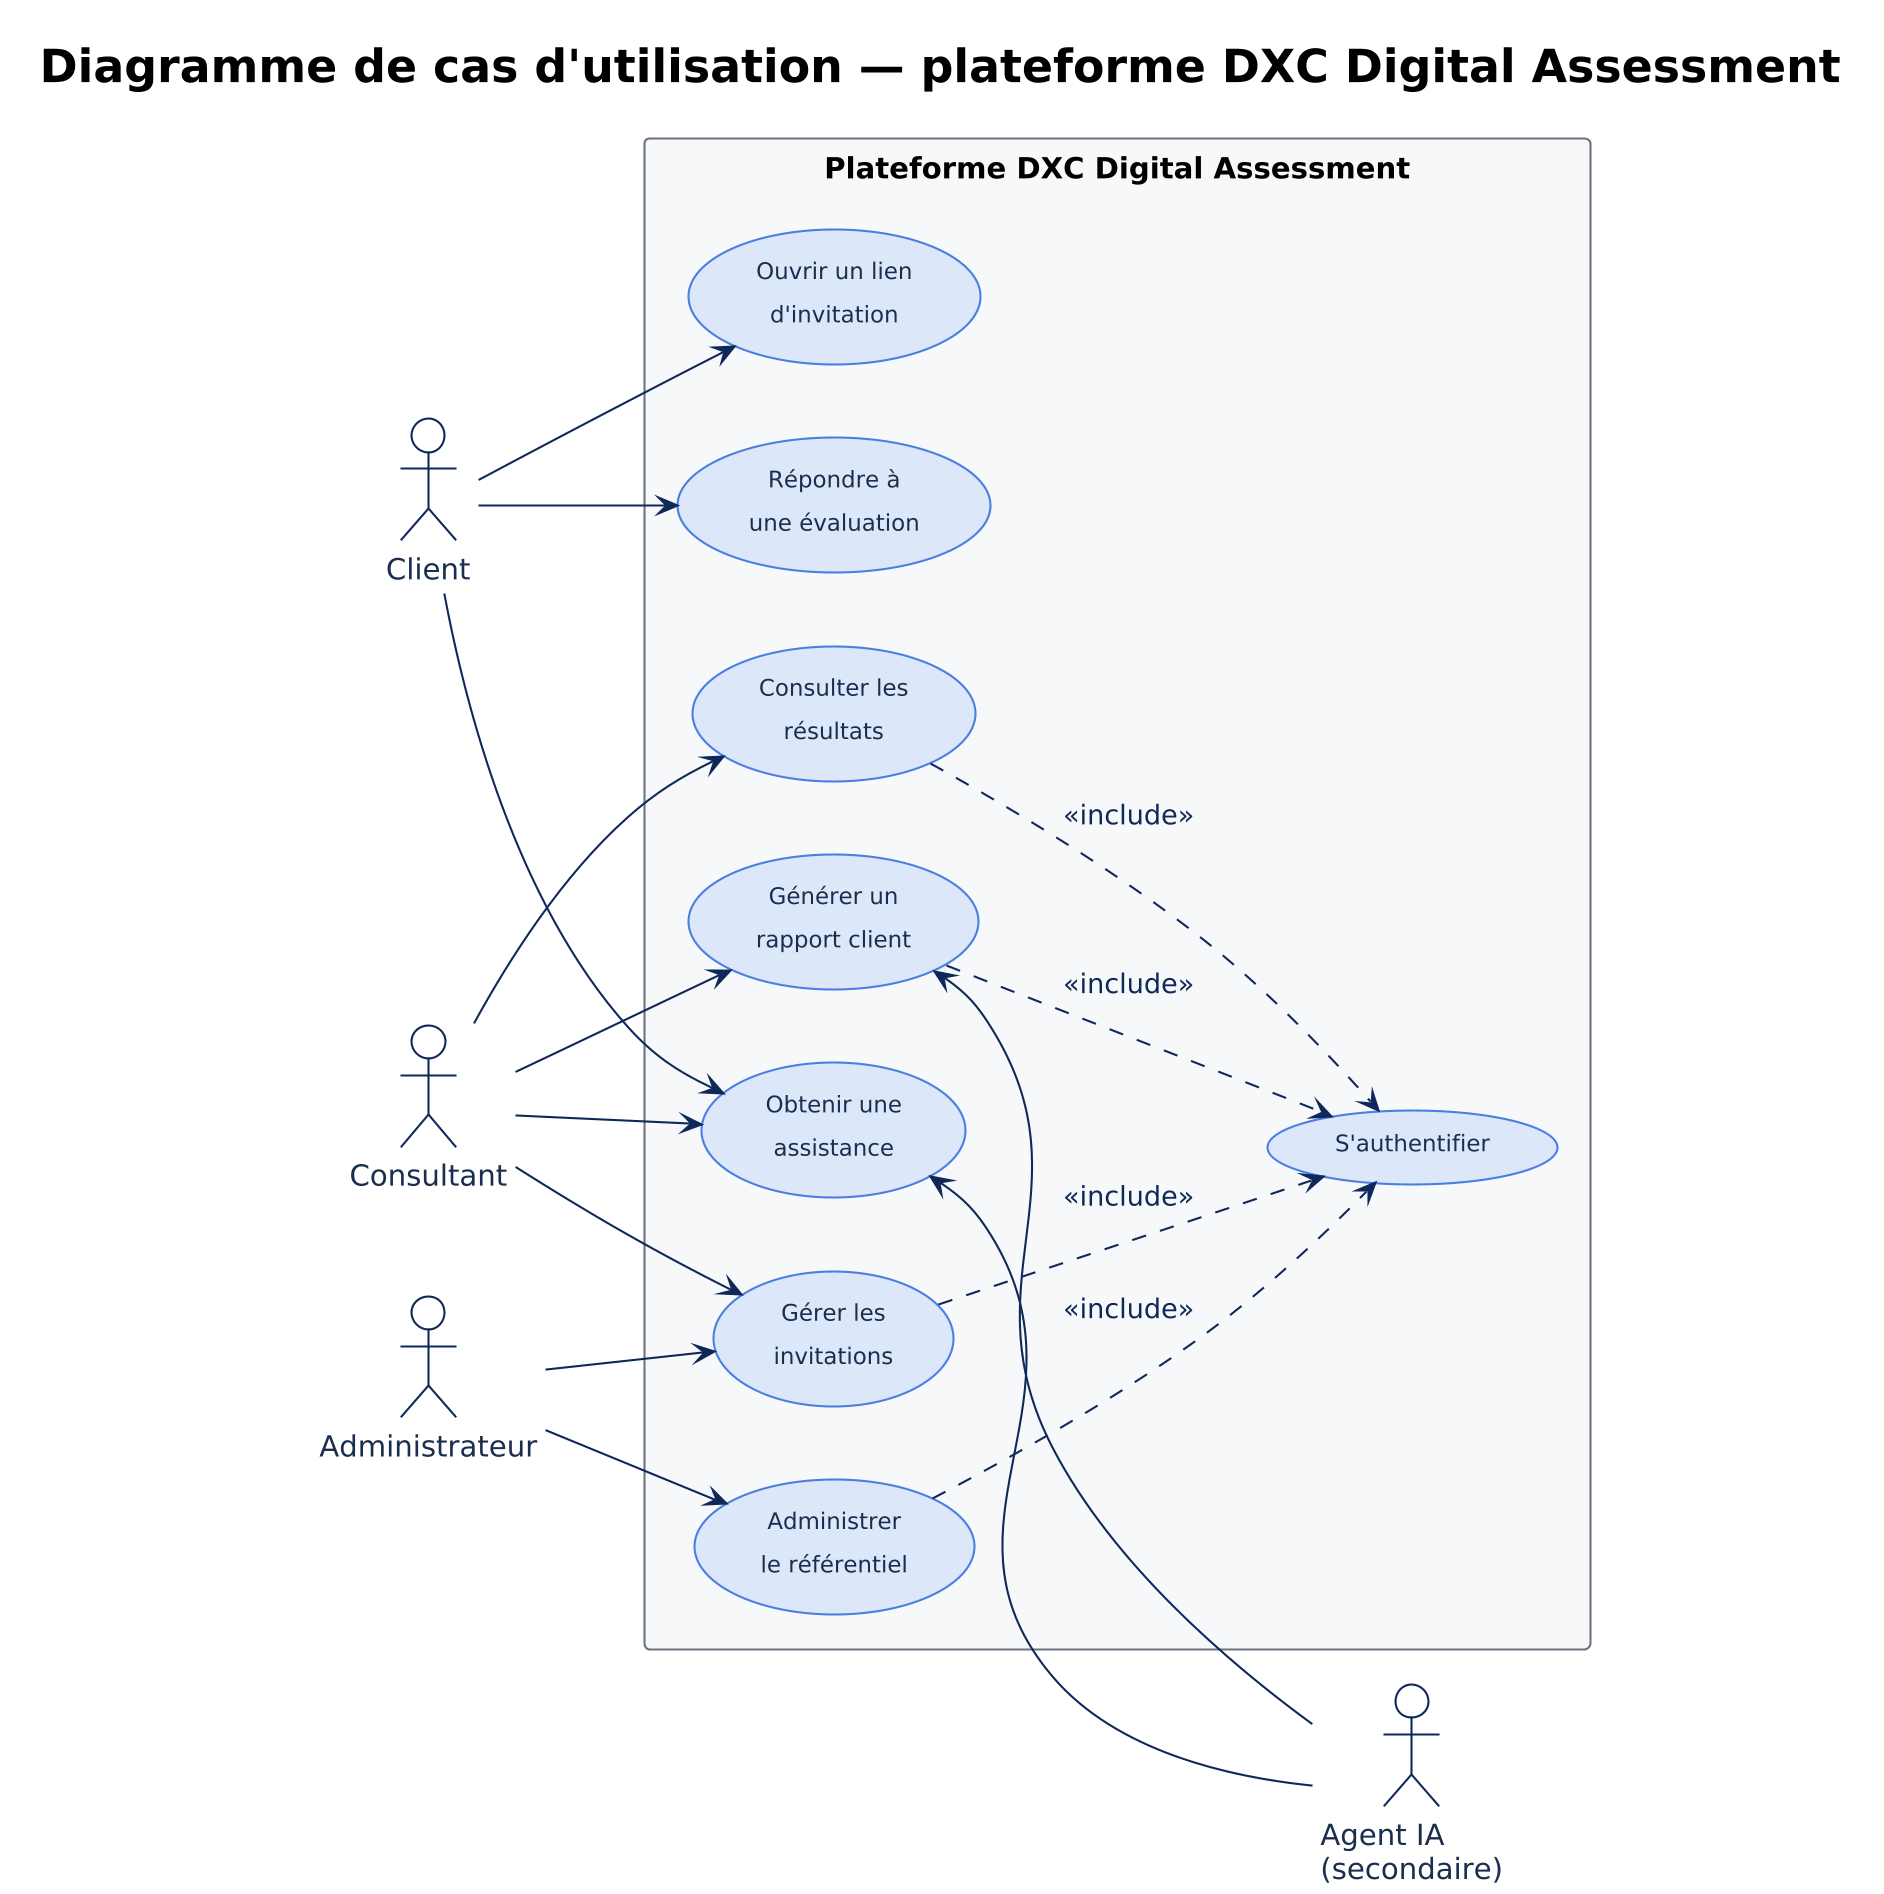
\includegraphics[width=\textwidth, height=0.78\textheight, keepaspectratio]{figures/uml-usecase.png}
\caption[Diagramme de cas d'utilisation]{Diagramme de cas d'utilisation UML synthétisant les interactions principales avec la plateforme. Le client accède à une évaluation via un lien d'invitation, le consultant exploite les résultats et déclenche les rapports, l'administrateur étend le périmètre du consultant à la gestion du référentiel, et l'Agent IA intervient comme acteur secondaire dans la génération de rapports et l'assistance contextuelle. Les relations \textit{«\,include\,»} en pointillés rappellent que les cas réservés impliquent une authentification préalable.}
\label{fig:usecase}
\end{figure}

\begin{table}[H]
\centering
\caption{Description synthétique des principaux cas d'utilisation.}
\begin{tabularx}{\textwidth}{>{\bfseries}L{4cm}Y}
\toprule
Cas d'utilisation & Description \\
\midrule
Répondre à une évaluation & Le client accède au questionnaire, répond aux questions et soumet ses réponses. \\
Gérer le questionnaire & L'administrateur crée ou modifie les sections, questions, choix et traductions. \\
Analyser les résultats & Le consultant consulte les scores, filtres, graphiques, soumissions et exports. \\
Générer un rapport & Le consultant déclenche la génération d'un rapport assisté par le module IA. \\
Obtenir une assistance & L'utilisateur interagit avec le chat pour obtenir une aide contextuelle. \\
\bottomrule
\end{tabularx}
\end{table}

Les trois cas d'utilisation les plus critiques font l'objet d'une description détaillée ci-dessous, sous la forme de scénarios nominal et alternatif.

\begin{table}[H]
\centering
\caption{Cas d'utilisation détaillé~: répondre à une évaluation.}
\begin{tabularx}{\textwidth}{>{\bfseries}L{3.5cm}Y}
\toprule
Élément & Description \\
\midrule
Acteur principal & Client (répondant) \\
Préconditions & Le client dispose d'un lien d'invitation valide reçu par e-mail, ou accède directement à un parcours public. \\
Postconditions & Une soumission est persistée en base avec son score de maturité~; l'invitation, si elle est consommée, est marquée comme utilisée. \\
Scénario nominal &
1. Le client ouvre le lien d'invitation et atterrit sur la page d'accueil. \newline
2. Il sélectionne la langue (FR / EN / AR). \newline
3. Il lit la page de contexte de l'évaluation. \newline
4. Il répond aux questions par section, en suivant la progression. \newline
5. Il confirme et soumet ses réponses. \newline
6. Le backend calcule le score de maturité et persiste la soumission. \newline
7. Le client est redirigé vers une page de remerciement. \\
Scénario alternatif &
2a. L'invitation est expirée ou révoquée~: la plateforme affiche une page d'erreur explicite et interrompt le parcours. \newline
5a. Une question obligatoire n'a pas été répondue~: le système signale la section concernée et empêche la soumission. \\
\bottomrule
\end{tabularx}
\label{tab:uc-respond}
\end{table}

\begin{table}[H]
\centering
\caption{Cas d'utilisation détaillé~: gérer les invitations.}
\begin{tabularx}{\textwidth}{>{\bfseries}L{3.5cm}Y}
\toprule
Élément & Description \\
\midrule
Acteur principal & Consultant authentifié \\
Préconditions & Le consultant est connecté via SSO Keycloak avec un rôle \texttt{EXPERT} ou \texttt{ADMIN}. \\
Postconditions & Une nouvelle invitation est créée et son lien est utilisable~; le consultant peut ensuite la suivre ou la prolonger. \\
Scénario nominal &
1. Le consultant ouvre l'écran de gestion des invitations. \newline
2. Il sélectionne un client, un domaine et un type d'évaluation. \newline
3. Il fournit l'adresse e-mail du répondant et choisit éventuellement les sections autorisées. \newline
4. Il valide la création. \newline
5. Le backend persiste l'invitation et déclenche l'envoi du courriel SMTP. \newline
6. Le statut \textit{pending} apparaît dans le tableau de suivi. \\
Scénario alternatif &
5a. L'envoi SMTP échoue~: l'invitation reste persistée mais une alerte invite le consultant à relancer manuellement. \newline
6a. Le consultant peut prolonger la date d'expiration ou révoquer une invitation à tout moment. \\
\bottomrule
\end{tabularx}
\label{tab:uc-invite}
\end{table}

\begin{table}[H]
\centering
\caption{Cas d'utilisation détaillé~: générer un rapport client.}
\begin{tabularx}{\textwidth}{>{\bfseries}L{3.5cm}Y}
\toprule
Élément & Description \\
\midrule
Acteur principal & Consultant authentifié \\
Acteur secondaire & Agent IA \\
Préconditions & Au moins une soumission est disponible pour le client ciblé. \\
Postconditions & Un rapport au statut \texttt{DRAFT} est associé à la soumission~; le consultant peut le télécharger, l'éditer puis le partager. \\
Scénario nominal &
1. Depuis le tableau de bord analytique, le consultant sélectionne un client. \newline
2. Il clique sur «~Générer un rapport~». \newline
3. Le frontend appelle l'Agent IA via le proxy Next.js. \newline
4. L'agent récupère les soumissions auprès du backend Spring Boot. \newline
5. L'agent construit un prompt structuré, appelle Mistral et retourne le rapport au format PDF. \newline
6. Le rapport est sauvegardé avec le statut \texttt{DRAFT} et proposé au téléchargement. \\
Scénario alternatif &
3a. L'Agent IA met plus de temps que prévu~: l'interface affiche un état de chargement explicite et n'autorise pas la double génération. \newline
5a. L'appel au modèle échoue~: un message d'erreur informatif est affiché et le rapport n'est pas persisté. \\
\bottomrule
\end{tabularx}
\label{tab:uc-report}
\end{table}

\section{Modèle conceptuel des données}
La base de données est construite autour de plusieurs entités métier : type d'évaluation, domaine, section, question, choix, invitation, soumission, réponse et rapport. Le diagramme de classes suivant ne présente pas tous les attributs techniques, mais met en évidence les relations essentielles nécessaires à la compréhension du modèle.

\begin{figure}[p]
\centering
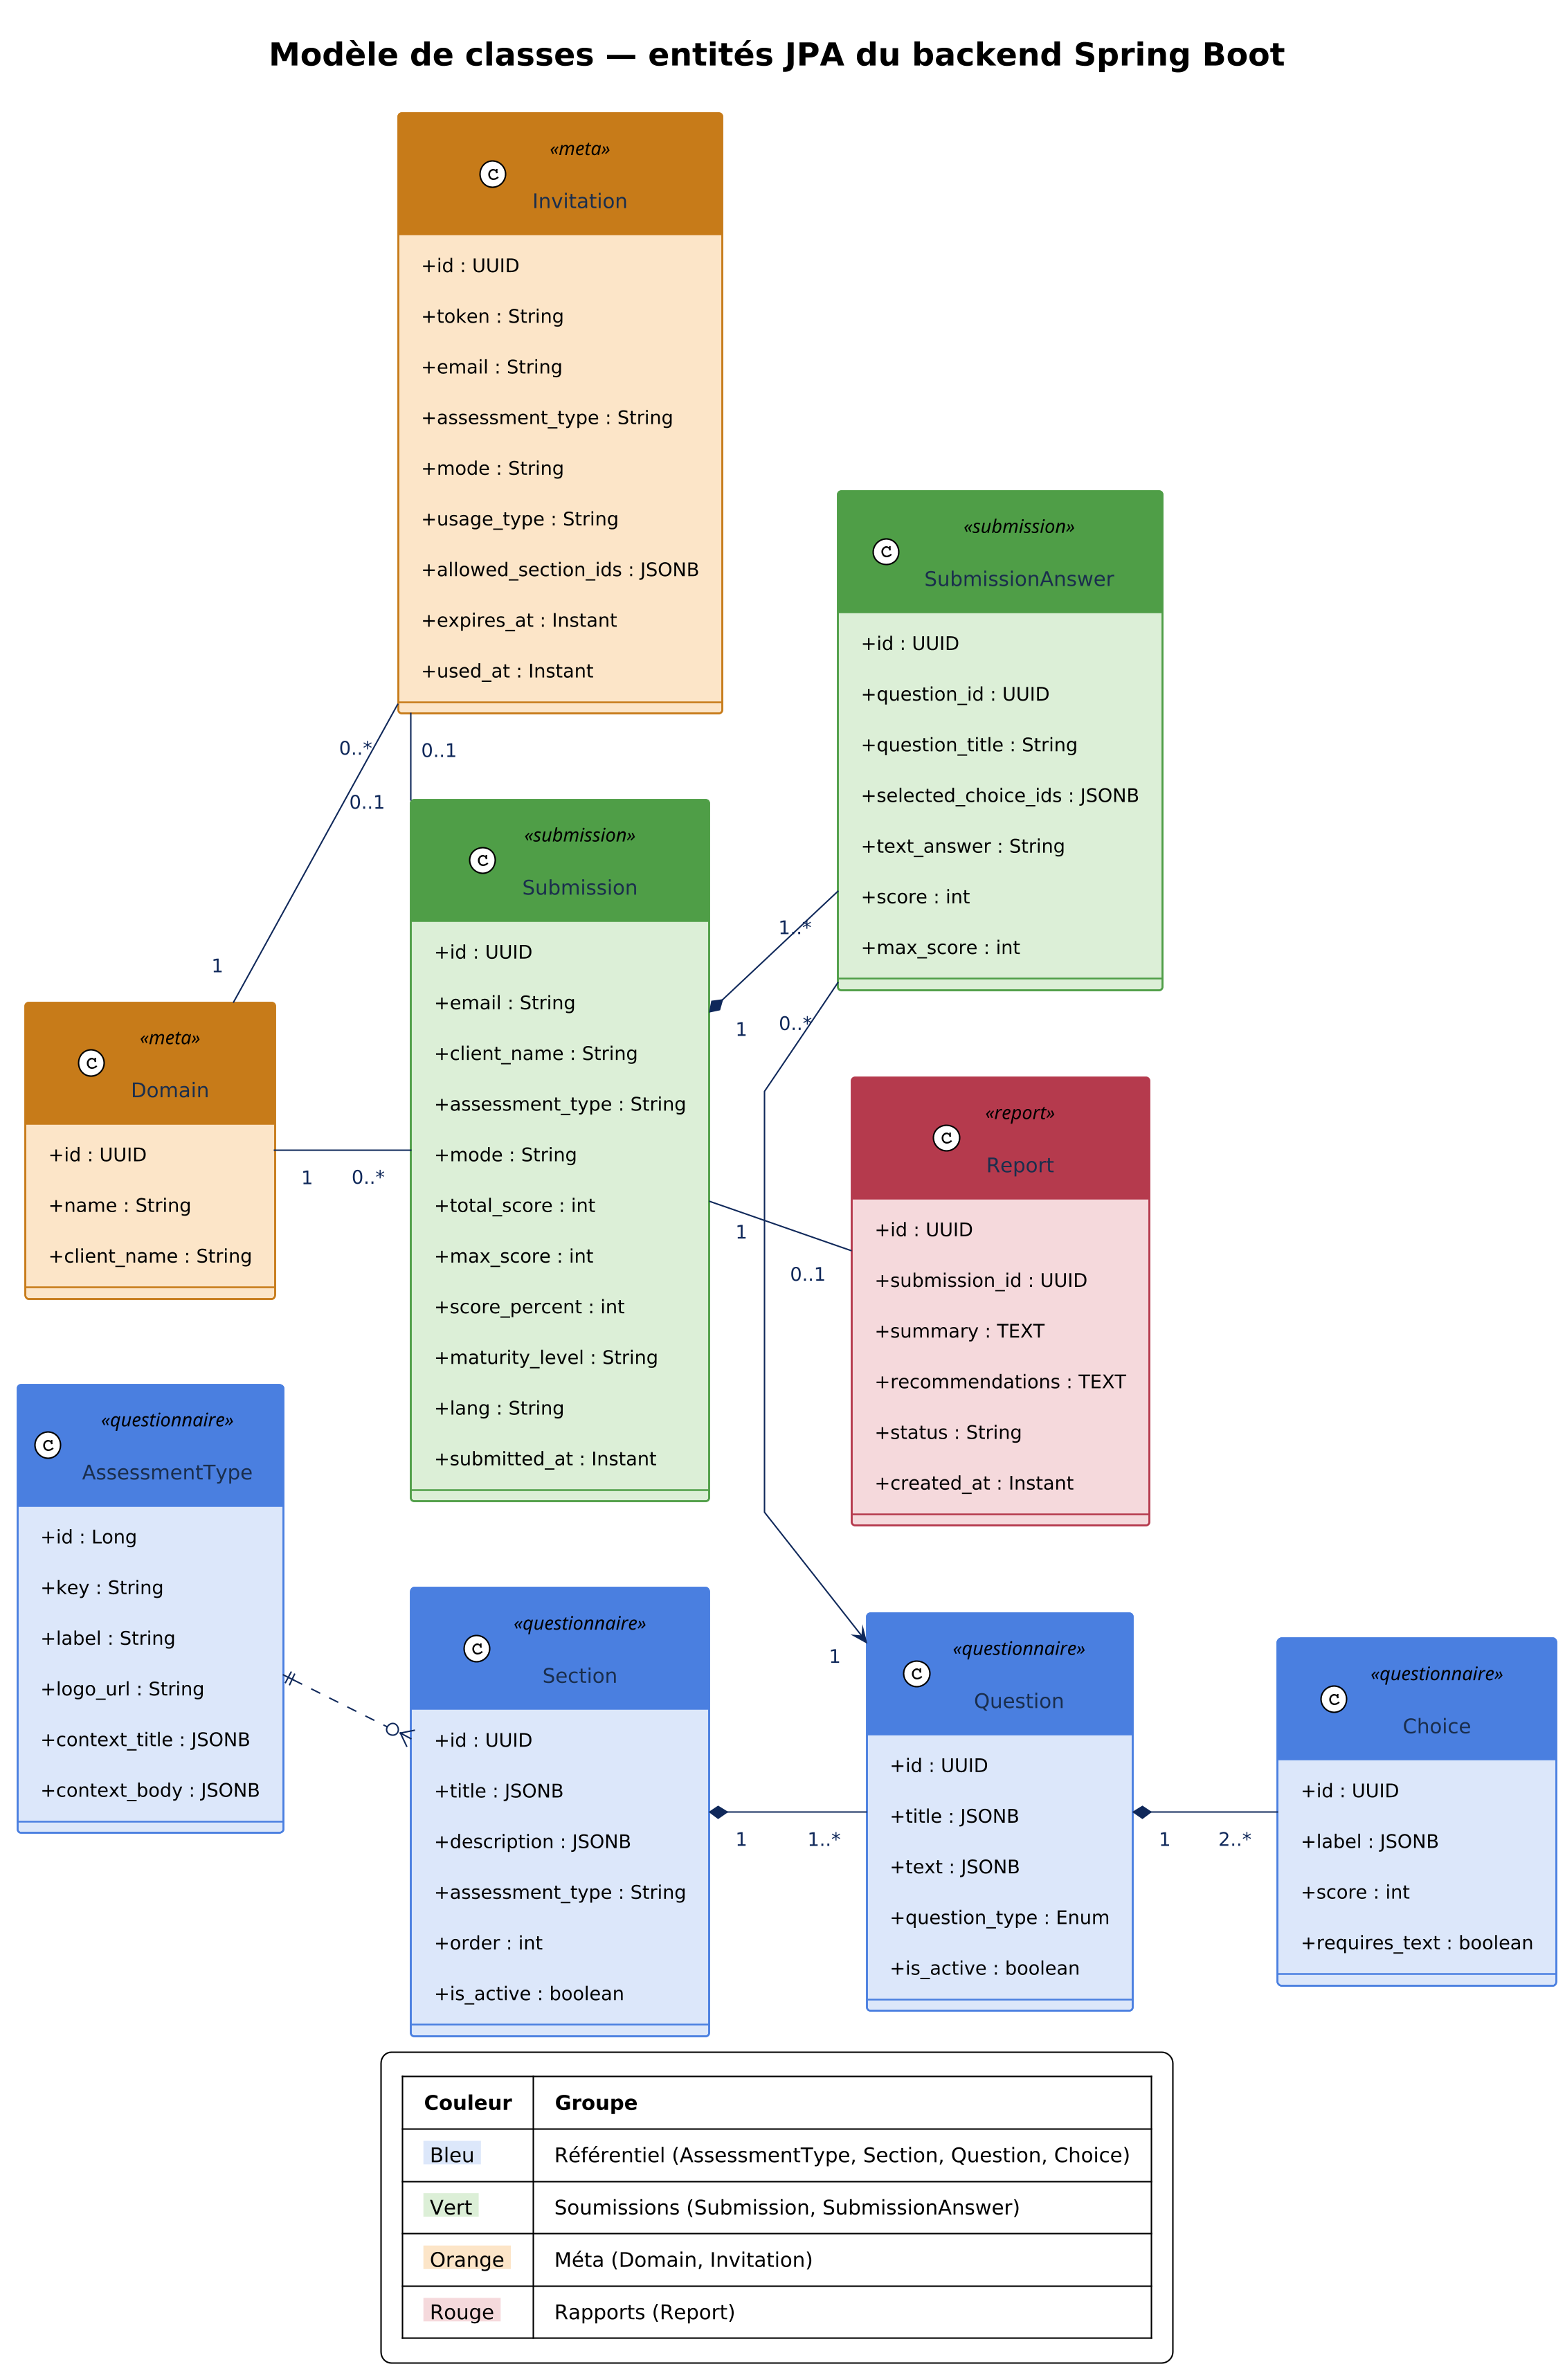
\includegraphics[width=\textwidth, height=0.85\textheight, keepaspectratio]{figures/uml-class.png}
\caption[Diagramme de classes du modèle métier]{Diagramme de classes UML simplifié du modèle métier. Les classes sont regroupées par couleur selon leur rôle~: questionnaire (bleu), soumissions (vert), méta (orange) et rapports (rouge). Les compositions (losange noir plein) signalent une dépendance d'existence~: les sections appartiennent à un type d'évaluation, les questions à une section, les choix à une question, les réponses et rapports à une soumission. Les associations simples relient un domaine à ses invitations et une invitation à la soumission qu'elle a permis de collecter.}
\label{fig:modele}
\end{figure}

\section{Parcours utilisateur}
Le parcours client débute par la sélection d'une évaluation ou l'ouverture d'un lien d'invitation. Le système affiche ensuite une page de contexte, puis les questions organisées par sections. À la soumission, les réponses sont envoyées au backend, qui calcule les scores et enregistre la soumission.

Le parcours administrateur commence par l'authentification. Une fois connecté, l'administrateur peut gérer les questionnaires, créer des invitations, lancer des évaluations internes et consulter les résultats dans le tableau de bord analytique.

Le diagramme de séquence ci-dessous représente le scénario principal autour d'une invitation. Il montre la succession des échanges entre les acteurs et le backend, depuis la création de l'invitation jusqu'à l'exploitation des résultats.

\begin{figure}[p]
\centering
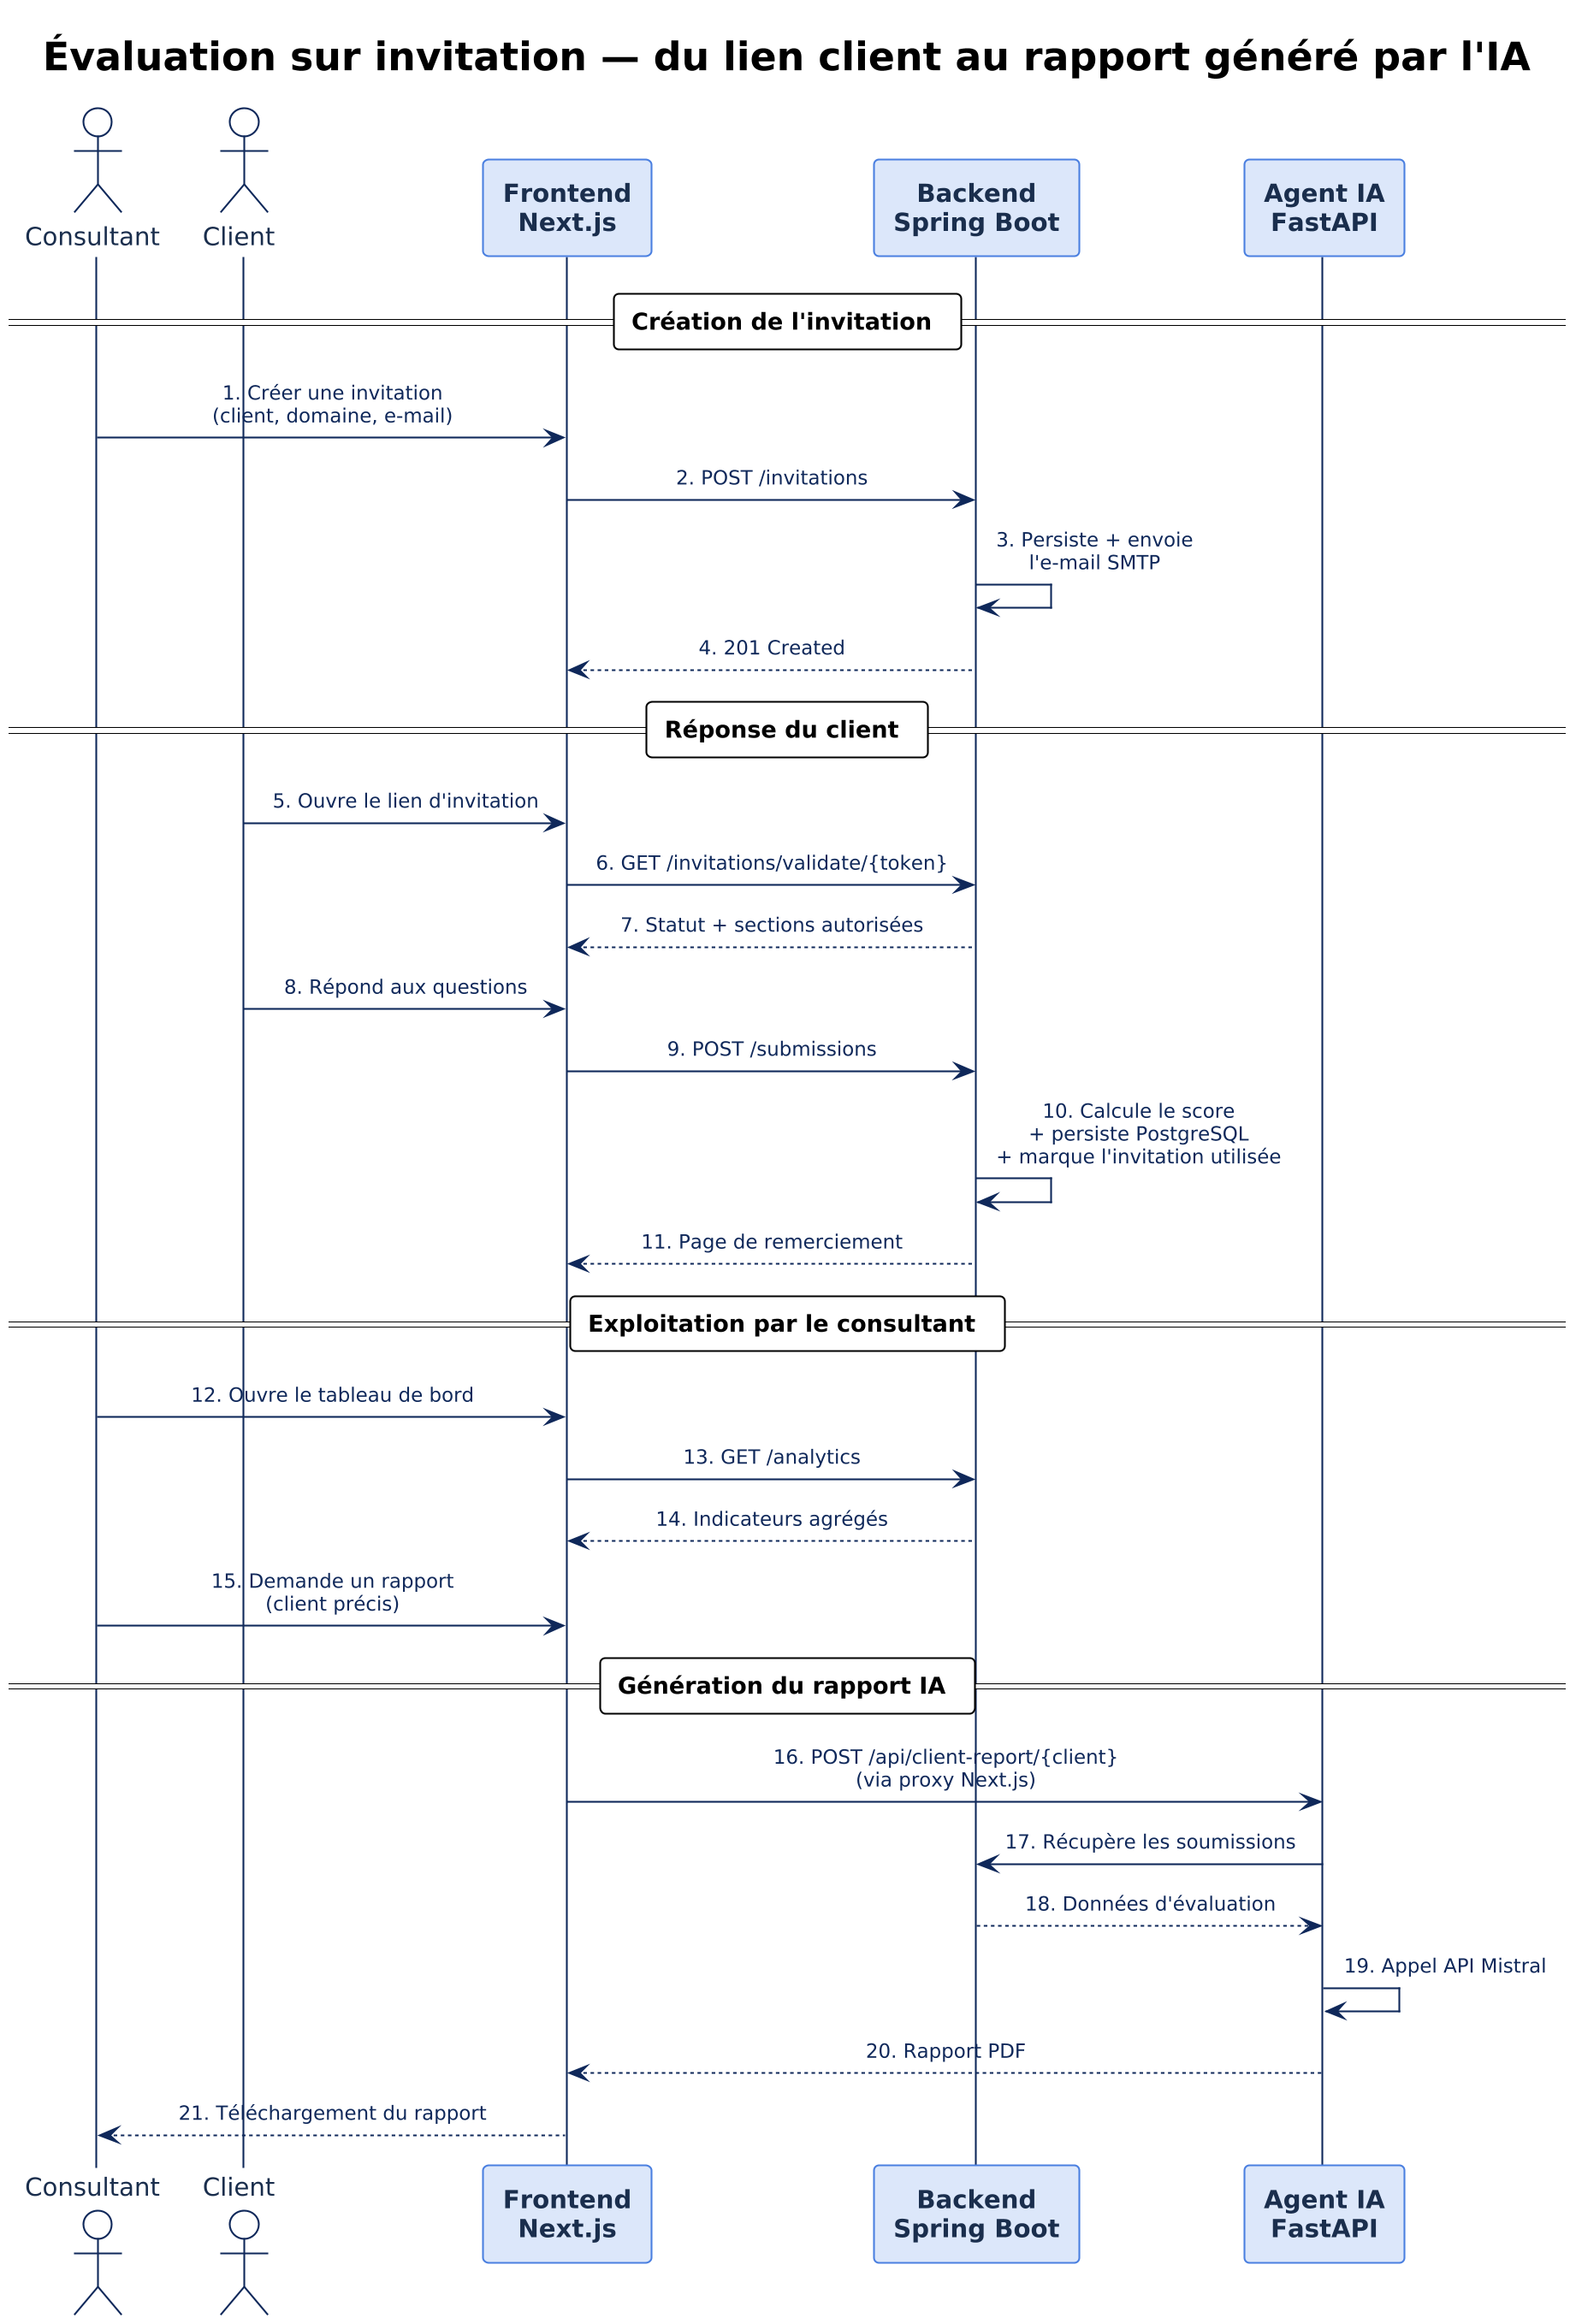
\includegraphics[width=\textwidth, height=0.85\textheight, keepaspectratio]{figures/uml-sequence.png}
\caption[Diagramme de séquence du parcours principal]{Diagramme de séquence UML du parcours nominal, du lien d'invitation au rapport généré par l'Agent IA. Le scénario se décompose en quatre phases~: création de l'invitation par le consultant, réponse du client (validation du jeton, soumission, scoring), exploration des résultats par le consultant dans le tableau de bord, puis génération à la demande d'un rapport client (le frontend passe par le proxy Next.js, l'Agent IA récupère les soumissions auprès du backend et délègue la rédaction à Mistral).}
\label{fig:parcours-global}
\end{figure}

\section{Conclusion}
Ce chapitre a fixé les besoins, les acteurs, les règles métier et les entités principales du système. Ces éléments servent de référence pour l'architecture technique présentée au chapitre suivant.

\chapter{Étude technique}
\chapterintro{Ce chapitre décrit l'architecture multi-services retenue, justifie le choix des technologies à chaque étage du système et explique comment les composants (frontend, API, base de données, authentification, Agent IA) communiquent entre eux.}

\section{Architecture globale}
La plateforme adopte une architecture multi-services, où chaque composant a un rôle bien délimité~: le frontend s'occupe de l'expérience utilisateur, le backend héberge la logique métier et l'accès aux données, la base PostgreSQL assure la persistance, Keycloak prend en charge l'authentification et l'autorisation, et l'Agent IA expose ses services en marge des flux principaux. Ce découplage a été retenu pour deux raisons~: il permet de faire évoluer une couche sans toucher aux autres, et il facilite le travail en parallèle sur la même solution. La figure~\ref{fig:architecture} restitue cette organisation et les protocoles d'échange entre composants.

\begin{figure}[!htbp]
\centering
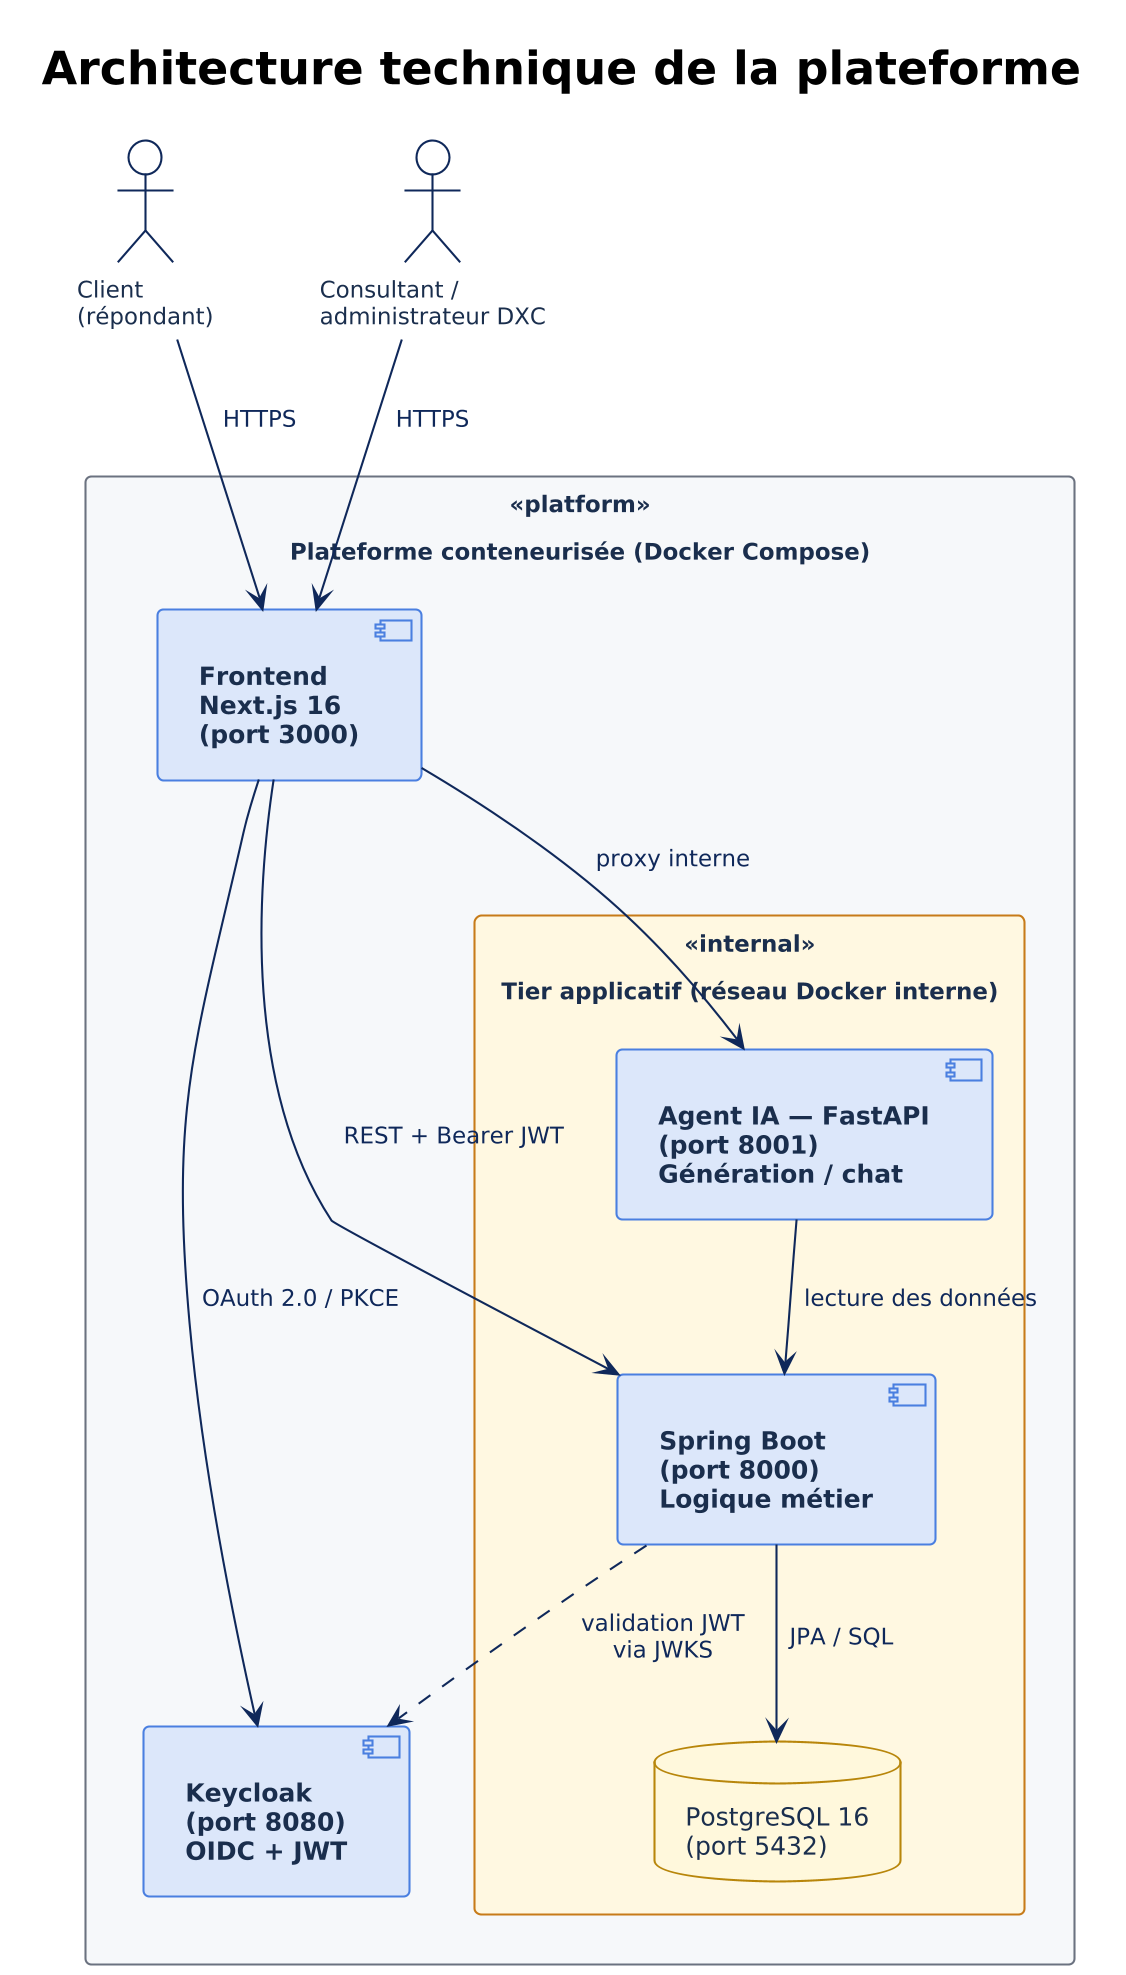
\includegraphics[width=0.72\textwidth]{figures/uml-architecture.png}
\caption[Diagramme de composants de la plateforme]{Diagramme de composants UML de la plateforme. Le frontend Next.js (port 3000), le backend Spring Boot (port 8000), le service Agent IA FastAPI (port 8001) et Keycloak (port 8080) sont représentés comme des composants conteneurisés Docker. PostgreSQL (port 5432) figure sous sa notation cylindrique. Les flèches précisent les protocoles d'échange~: HTTPS et OAuth2 + PKCE pour l'authentification, REST/JSON pour les appels métier, JPA/SQL pour la persistance, et JWT/JWKS pour la validation des jetons. L'Agent IA, isolé sur le réseau interne du backend, n'est joignable qu'à travers le frontend.}
\label{fig:architecture}
\end{figure}

\section{Justification des choix technologiques}
Le choix de la pile technologique engage la maintenabilité du produit, la courbe d'apprentissage pour de futurs contributeurs et la capacité à le faire évoluer. Chaque brique a été retenue pour répondre à un besoin précis~: construire une interface réactive et maintenable, exposer une API métier sécurisée, stocker des données structurées et fortement reliées, gérer une authentification fédérée conforme aux standards et accueillir un service IA évoluant à part.

Les décisions s'appuient sur les documentations officielles des outils utilisés~: Next.js, React et TypeScript pour le frontend, Spring Boot pour le backend, PostgreSQL pour la persistance, Keycloak pour l'identité, FastAPI pour l'Agent IA et Docker pour l'orchestration locale \cite{nextjs,react,typescript,springboot,keycloak,postgresql,fastapi,docker}. Des références complémentaires ont guidé la modélisation UML \cite{larman2012}, les principes de réécriture incrémentale appliqués aux services métier \cite{fowler2018}, l'usage de Recharts pour la visualisation \cite{recharts}, l'intégration d'Auth.js comme client OIDC côté Next.js \cite{authjs} et le cadrage méthodologique inspiré de Scrum \cite{scrum}. La figure~\ref{fig:tech-stack} récapitule visuellement la pile retenue.

\begin{figure}[H]
\centering
\renewcommand{\arraystretch}{1.3}
\begin{tabular}{>{\centering\arraybackslash}m{2.0cm} >{\bfseries}m{2.4cm} >{\RaggedRight\arraybackslash}m{8.5cm}}

\includegraphics[height=1.1cm,keepaspectratio]{figures/logos/nextdotjs.png}  & Next.js 16 & Framework React de référence pour le rendu serveur et le routage applicatif côté frontend. \\

\includegraphics[height=1.1cm,keepaspectratio]{figures/logos/react.png}       & React 19 & Bibliothèque de composants déclaratifs pour la construction des interfaces utilisateur. \\

\includegraphics[height=1.1cm,keepaspectratio]{figures/logos/typescript.png}  & TypeScript & Surcouche typée de JavaScript pour la fiabilité des contrats de données. \\

\includegraphics[height=1.1cm,keepaspectratio]{figures/logos/springboot.png}  & Spring Boot 3 & Framework Java pour l'exposition de l'API REST, la sécurité et la persistance JPA. \\

\includegraphics[height=1.1cm,keepaspectratio]{figures/logos/postgresql.png}  & PostgreSQL 16 & SGBD relationnel pour le stockage transactionnel et le support natif de \texttt{JSONB}. \\

\includegraphics[height=1.1cm,keepaspectratio]{figures/logos/keycloak.png}    & Keycloak & Fournisseur d'identité OpenID Connect pour l'authentification SSO et la gestion des rôles. \\

\includegraphics[height=1.1cm,keepaspectratio]{figures/logos/fastapi.png}     & FastAPI & Framework Python asynchrone exposant les endpoints de l'Agent IA. \\

\includegraphics[height=1.1cm,keepaspectratio]{figures/logos/python.png}      & Python 3.12 & Langage du module Agent IA, des prompts et de l'orchestration LLM. \\

\includegraphics[height=1.1cm,keepaspectratio]{figures/logos/docker.png}      & Docker Compose & Orchestration locale des cinq services dans des conteneurs isolés. \\

\includegraphics[height=1.1cm,keepaspectratio]{figures/logos/github.png}      & GitHub Actions & Pipeline d'intégration continue déclenchée à chaque \textit{push} et \textit{pull request}. \\

\includegraphics[height=1.1cm,keepaspectratio]{figures/logos/caddy.png}       & Caddy & Reverse proxy HTTPS de production, certificats Let's Encrypt automatiques via ACME. \\
\end{tabular}
\caption[Pile technologique de la plateforme]{Pile technologique de la plateforme, du frontend à la mise en production~: rôle assuré par chaque brique et logo officiel correspondant.}
\label{fig:tech-stack}
\end{figure}

\section{Frontend Next.js}
Le frontend s'appuie sur Next.js~16 avec React~19 et TypeScript. Ce trio offre un bon compromis entre la productivité de développement (routeur intégré, conventions de fichiers, génération de pages côté serveur quand c'est utile) et la rigueur du typage statique, précieuse dans une application où les données métier circulent entre une dizaine d'écrans hétérogènes.

Concrètement, le frontend porte les pages publiques et les parcours d'évaluation, gère l'état local des réponses et la progression au sein du questionnaire, dialogue avec le backend pour persister les soumissions, héberge l'espace administrateur et le constructeur de questionnaires, expose les visualisations analytiques basées sur Recharts, et orchestre les appels vers l'Agent IA à travers un proxy Next.js. Il porte également l'essentiel de l'expérience multilingue et l'adaptation responsive aux différentes tailles d'écran.

\begin{table}[H]
\centering
\caption{Organisation des principaux modules frontend et responsabilités associées.}
\begin{tabularx}{\textwidth}{>{\bfseries}L{4.7cm}Y}
\toprule
Module frontend & Responsabilité \\
\midrule
Page d'accueil & Choix de l'évaluation et orientation vers les parcours. \\
Composant d'évaluation & Affichage du questionnaire, progression, collecte et soumission des réponses. \\
Espace administrateur & Constructeur de sections, questions, choix et contexte d'évaluation. \\
Gestion des invitations & Création, suivi, renvoi et gestion d'expiration des invitations. \\
Tableau de bord analytique & Indicateurs, filtres, visualisations, détails de soumission et rapports. \\
Client Agent IA & Intégration avec le service Agent IA via le proxy Next.js. \\
Contexte de langue & Gestion des traductions et de la direction d'affichage RTL. \\
\bottomrule
\end{tabularx}
\label{tab:frontend-modules}
\end{table}

L'organisation retenue sépare les pages, les composants réutilisables, les utilitaires et les contextes. Cette séparation évite de mélanger les écrans d'administration, les parcours d'évaluation et le tableau de bord analytique dans une même couche de code.

La logique frontend suit un découpage clair : les pages pilotent les parcours, les composants affichent les éléments d'interface, les utilitaires transforment les données et les clients API assurent la communication avec les services externes. Ce découpage facilite l'évolution de modules différents sans regrouper l'ensemble de la logique dans les mêmes fichiers.

\begin{table}[H]
\centering
\caption{Niveaux d'organisation de la partie frontend.}
\begin{tabularx}{\textwidth}{>{\bfseries}L{3.5cm}Y}
\toprule
Niveau & Rôle \\
\midrule
Pages & Entrées principales des parcours : accueil, évaluation, administration, invitations et analyse. \\
Composants & Éléments réutilisables : cartes, formulaires, tableaux, modales, filtres et visualisations. \\
Contextes & Gestion de la langue, de certaines préférences d'affichage et des états partagés. \\
Utilitaires & Fonctions de formatage, d'agrégation, d'export et de préparation des données. \\
Clients API & Appels aux endpoints backend et aux routes proxy vers le module Agent IA. \\
\bottomrule
\end{tabularx}
\end{table}

\section{Choix d'ergonomie frontend}
L'ergonomie a été adaptée aux différents profils. Pour le client, le questionnaire devait rester clair, linéaire et facile à terminer. Pour le consultant, les écrans devaient offrir un accès rapide aux filtres, aux soumissions et aux indicateurs. Cette différence explique la présence de parcours guidés côté client et d'interfaces plus denses côté administration et analyse.

Les choix d'ergonomie se traduisent par un affichage progressif des questions, des filtres et des onglets dans le tableau de bord, des badges de statut pour les invitations, ainsi que des graphiques et heatmaps pour repérer les scores faibles. Une partie importante du travail a aussi concerné l'adaptation responsive et le support RTL, pour éviter une expérience dégradée sur petit écran ou en langue arabe.

\section{Backend Spring Boot}
Le backend Spring Boot porte la logique métier de la plateforme. Il expose les endpoints REST, applique les règles de validation, calcule les scores de maturité et accède à la base de données via Spring Data JPA. Le choix de Spring Boot, plutôt qu'un framework plus léger, tient à la maturité de son écosystème (sécurité, observabilité, JPA, gestion des transactions) et au fait qu'une partie du métier (invitations à usage unique, soumissions à scorer, calculs d'agrégats) tire parti de cette robustesse.

Les contrôleurs sont organisés par domaine fonctionnel~: évaluations, soumissions, invitations, administration du référentiel, analytics, rapports et types d'évaluation. Les services regroupent la logique métier proprement dite, tandis que les repositories restent volontairement fins, dédiés à l'accès aux données. Le backend fait partie intégrante du périmètre applicatif réalisé~: il a été pensé conjointement avec le frontend, et son contrat d'API a évolué au rythme des besoins d'écrans, en particulier ceux du tableau de bord analytique qui condense soumissions, scores et filtres.

\section{Authentification avec Keycloak}
La gestion des identités est externalisée à Keycloak, ce qui présente un double intérêt~: éviter de réinventer un système d'authentification propre à l'application et bénéficier nativement des fonctions standard (SSO, gestion des rôles, intégration future avec un annuaire d'entreprise). Côté frontend, Auth.js prend en charge le flux OAuth2~\cite{rfc6749} avec PKCE~\cite{rfc7636}, gère le cycle de vie des jetons et leur rafraîchissement. Côté backend, Spring Security en mode \textit{OAuth2 Resource Server} valide chaque jeton JWT~\cite{rfc7519} entrant via le \textit{JSON Web Key Set} exposé par Keycloak et convertit les rôles du realm en autorités Spring exploitables dans les annotations de sécurité.

La sécurité ne s'arrête pas à l'écran de connexion. Les routes administrateur sont protégées côté interface par un \textit{middleware} Next.js et côté backend par les filtres Spring Security~; les jetons sont validés avant tout accès à une ressource sensible, et le périmètre de consultation est restreint au profil de l'utilisateur. Ce dernier point compte pour les tableaux de bord, qui agrègent des informations issues de plusieurs clients~: un consultant n'a accès qu'au périmètre qui le concerne.

\begin{figure}[p]
\centering
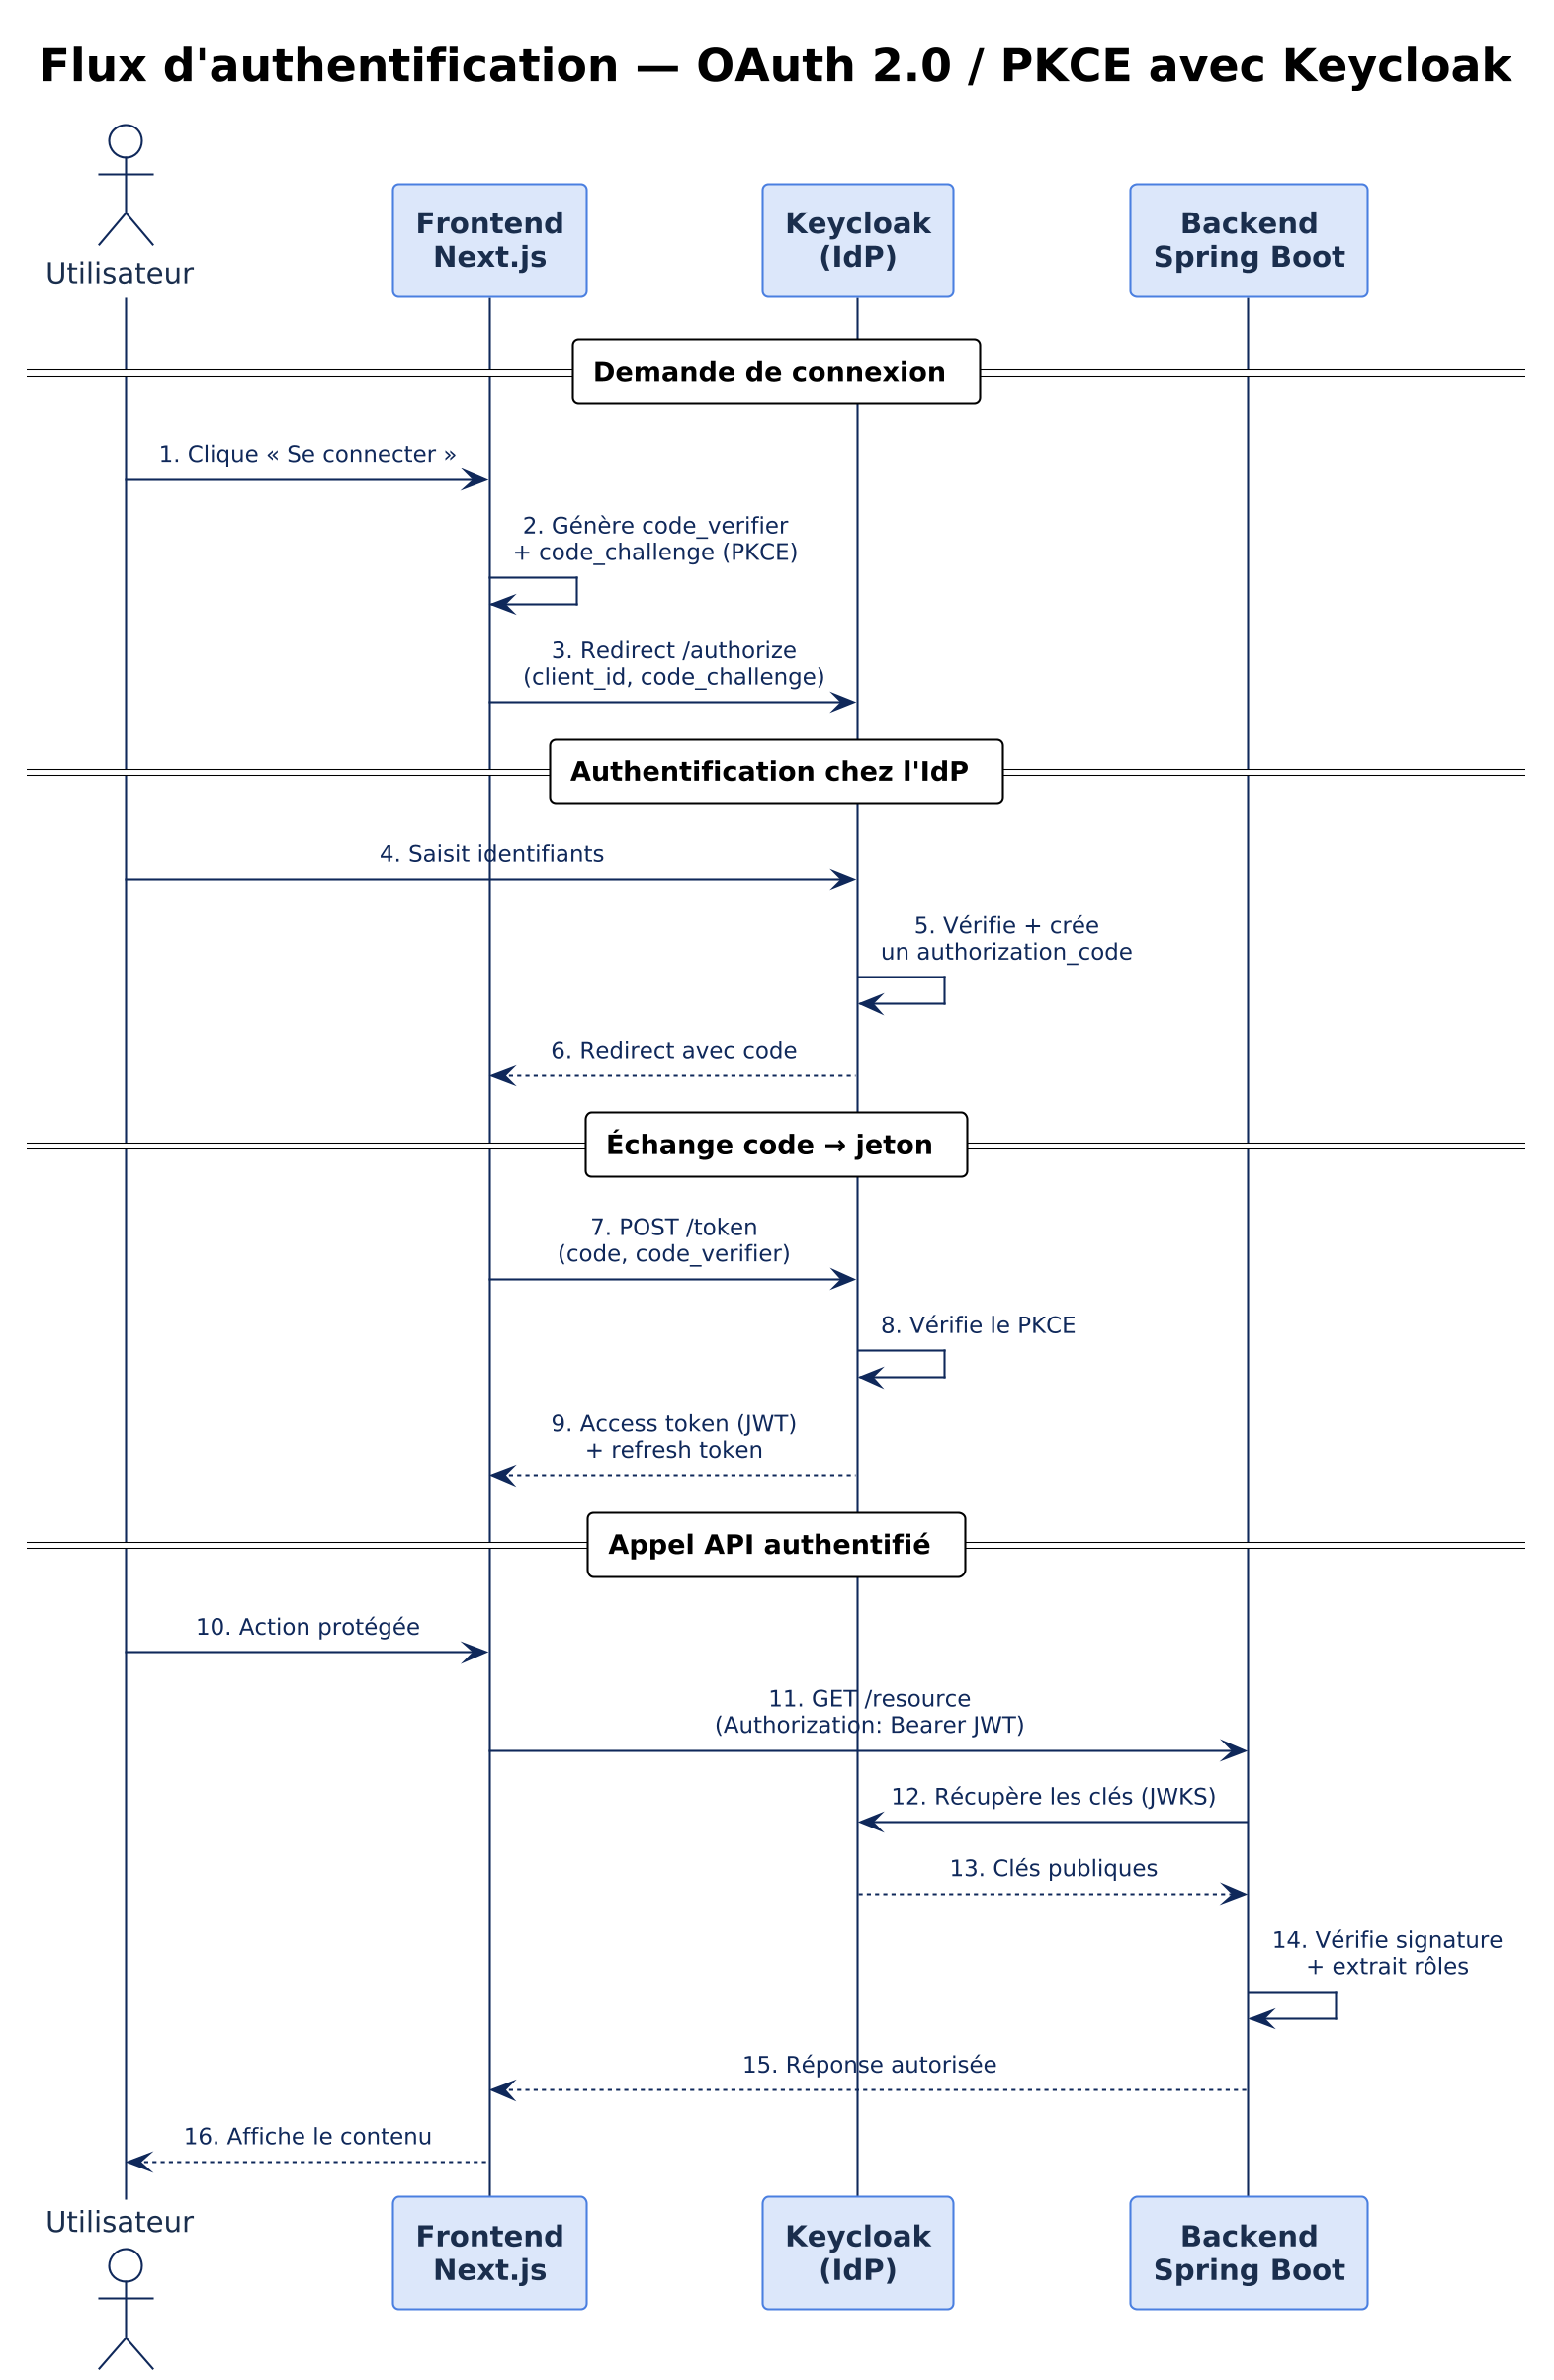
\includegraphics[width=\textwidth, height=0.85\textheight, keepaspectratio]{figures/uml-auth-sequence.png}
\caption[Flux d'authentification Keycloak]{Diagramme de séquence UML du flux d'authentification OAuth 2.0 avec PKCE. Le scénario se décompose en quatre phases~: demande de connexion (le frontend génère un \texttt{code\_verifier} et un \texttt{code\_challenge}), authentification chez l'IdP Keycloak, échange du \textit{code} contre un jeton JWT signé, puis appel d'une API protégée avec validation de la signature par le backend via l'endpoint JWKS de Keycloak.}
\label{fig:keycloak}
\end{figure}

\section{Module Agent IA}
Le module Agent IA, développé en FastAPI par Hiba Bouhnin, s'interface avec le backend pour récupérer les données d'évaluation nécessaires à ses traitements, et expose à son tour des endpoints consommés par le frontend pour afficher des synthèses, des recommandations, des rapports PDF et une assistance conversationnelle. Cette indépendance technique est précieuse~: elle permet de faire évoluer la couche IA sans toucher au backend métier, et inversement.

L'implémentation actuelle combine deux modèles aux finalités distinctes~: Mistral est mobilisé pour la génération de contenus analytiques structurés (recommandations, rapports) où la qualité du raisonnement prime sur la latence, tandis que Groq alimente l'assistance conversationnelle, où l'enjeu est avant tout d'obtenir une réponse rapide pour fluidifier le dialogue. Ma contribution sur ce volet s'est concentrée sur l'intégration de bout en bout~: préparer les données nécessaires côté backend, consommer les endpoints côté interface et gérer les états visibles par l'utilisateur (chargement, succès, erreur, indisponibilité).

Côté sécurité, l'Agent IA n'est pas exposé publiquement~: il n'est joignable que depuis le réseau Docker interne, et toutes les requêtes passent par un proxy Next.js qui sert d'unique point d'entrée. Ce choix réduit la surface d'attaque et empêche un appel direct aux endpoints internes depuis l'extérieur.

\begin{table}[H]
\centering
\caption{Répartition des responsabilités entre le frontend et le module Agent IA.}
\begin{tabularx}{\textwidth}{>{\bfseries}L{4cm}Y}
\toprule
Couche & Responsabilités \\
\midrule
Plateforme applicative & Fourniture des soumissions, scores, structures d'évaluation et données persistées ; déclenchement des générations, affichage des brouillons, gestion des états de chargement, téléchargement des PDF et affichage du chat. \\
Agent IA & Construction des prompts, appel aux modèles, agrégation IA, génération des recommandations et production des rapports. \\
\bottomrule
\end{tabularx}
\end{table}

\section{Persistance et orchestration locale}
PostgreSQL stocke l'ensemble des données métier~: types d'évaluation, sections, questions, choix, domaines, invitations, soumissions, réponses et rapports. Le choix d'une base relationnelle se justifie par la structure fortement reliée de ces données et par les besoins d'agrégation analytique, qui exigent souvent de regrouper les résultats par client, domaine, section ou type d'évaluation. Les attributs textuels multilingues sont stockés en \texttt{JSONB}, ce qui permet d'ajouter une langue sans modifier le schéma.

Côté orchestration, Docker Compose a servi tout au long du projet à lancer ensemble les cinq services nécessaires (PostgreSQL, Keycloak, Spring Boot, FastAPI et Next.js) avec leurs ports, leurs \textit{healthchecks} et leurs dépendances. Le déploiement local distingue les services exposés à l'utilisateur des services internes~: le frontend et Keycloak sont accessibles depuis l'extérieur, tandis que le backend et l'Agent IA communiquent sur le réseau Docker interne. Cette séparation se rapproche d'un environnement de production réel, ce qui a fiabilisé les tests d'intégration entre couches.

\section{Mise en production sur Azure}
La mise en production de la plateforme a été prise en charge par \textbf{Saad Khalmadani}, ingénieur DevOps chez DXC Technology, qui s'est greffé au projet pour porter la solution sur un environnement cloud opérationnel. L'infrastructure est provisionnée sur \textbf{Microsoft Azure} à l'aide de \textbf{Terraform}~: la définition des ressources (machine virtuelle, réseau, groupe de sécurité, DNS) est versionnée dans le dépôt et reproductible par une commande unique. La configuration applicative sur la VM est ensuite déroulée via un \textbf{playbook Ansible}, ce qui maintient le serveur dans un état déclaré et facilite les mises à jour.

Côté exposition publique, un \textbf{reverse proxy Caddy} agit comme unique point d'entrée HTTPS de la plateforme. Caddy démultiplexe les requêtes vers les services internes (\texttt{/auth} vers Keycloak, \texttt{/svc} vers le backend Spring Boot, le reste vers le frontend Next.js) et obtient automatiquement les certificats TLS auprès de \textbf{Let's Encrypt} via le protocole ACME, sans configuration manuelle. Le déploiement applicatif lui-même reste basé sur les images Docker construites par la pipeline d'intégration continue (voir section suivante), ce qui garantit que l'environnement de production reflète exactement les images validées en CI.

Ce volet sort du périmètre fonctionnel que j'ai porté, mais il complète la vue d'ensemble du projet et explique comment la plateforme est aujourd'hui accessible publiquement.

\section{Outillage de développement et intégration continue}
Le projet s'est appuyé sur un ensemble d'outils éprouvés du développement web et de la collaboration logicielle~: \textbf{Visual Studio Code} et \textbf{IntelliJ IDEA} pour l'édition de code, \textbf{Git} et \textbf{GitHub} pour le versionnement et la revue des contributions, \textbf{Docker Compose} pour l'orchestration locale, et les frameworks de tests propres à chaque couche (JUnit et Mockito côté backend, \texttt{node:assert} via \texttt{tsx} côté frontend, \texttt{pytest} et \texttt{ruff} côté agent).

Cet outillage est complété par une pipeline d'\textbf{intégration continue} GitHub Actions, déclenchée sur chaque \textit{push} et chaque \textit{pull request} ciblant la branche \texttt{main}. Elle se décompose en quatre \textit{jobs} parallèles couvrant les trois couches de l'application~:

\begin{table}[H]
\centering
\caption{Jobs de la pipeline GitHub Actions et vérifications associées.}
\begin{tabularx}{\textwidth}{>{\bfseries}L{3.6cm}Y}
\toprule
Job & Vérifications \\
\midrule
Frontend & Vérification stricte des types TypeScript (\texttt{tsc --noEmit}), exécution de la suite de tests analytiques, \textit{linting} ESLint et contrôle de formatage Prettier. \\
Backend & Compilation Maven, exécution des tests JUnit et empaquetage~: \texttt{mvn verify} avec mise en cache des dépendances Maven. \\
Agent IA & \textit{Linting} Python via \texttt{ruff check}, contrôle de formatage \texttt{ruff format --check} et exécution des tests Pytest. \\
Docker build & Construction des trois images Docker (frontend, backend, agent) afin de garantir que les \textit{Dockerfiles} restent cohérents avec le code et que toute régression de configuration est détectée en CI plutôt qu'en production. \\
\bottomrule
\end{tabularx}
\label{tab:ci-jobs}
\end{table}

La pipeline agit comme un filet de sécurité~: aucun changement n'atteint la branche principale sans avoir passé l'ensemble des contrôles. Elle aligne aussi les images Docker validées sur celles déployées en production, ce qui garde l'environnement local, l'environnement CI et l'environnement Azure sur la même base. Un extrait du fichier \texttt{ci.yml} figure en annexe pour référence.

\section{Stratégie de tests}
La stratégie de tests a été pensée pour combiner trois niveaux de garantie complémentaires~: des tests unitaires automatisés sur les fonctions critiques, des vérifications d'intégration entre couches, et des validations manuelles guidées par scénarios d'usage. Plutôt que viser une couverture exhaustive, on a privilégié la couverture des traitements à risque~: calcul des scores de maturité, consommation atomique des invitations, agrégations analytiques et exports.

Côté frontend, les tests portent sur la transformation des réponses en données affichables, l'export CSV, la persistance des brouillons de rapports et la synchronisation entre URL et stockage navigateur. Côté backend, ils valident les services métier (évaluations, soumissions, invitations, domaines), les calculs analytiques et les règles de sécurité. Les vérifications manuelles complètent l'ensemble sur les aspects difficilement automatisables~: rendu visuel, comportement responsive, états d'erreur et expérience multilingue, en particulier l'affichage RTL.

\begin{table}[H]
\centering
\caption{Synthèse des tests et vérifications réalisés durant le projet.}
\begin{tabularx}{\textwidth}{>{\bfseries}L{4cm}Y}
\toprule
Type de vérification & Objectif \\
\midrule
Tests frontend unitaires & Vérifier les fonctions d'agrégation, d'export CSV, de chargement des rapports et de formatage des réponses. \\
Tests backend unitaires & Valider les services métier, les calculs, la gestion des invitations et les règles de sécurité. \\
Tests d'intégration & Vérifier les échanges entre frontend, backend, Keycloak et Agent IA. \\
Tests responsive & Contrôler l'affichage sur desktop, tablette et mobile. \\
Tests fonctionnels & Valider les scénarios client, administrateur et consultant. \\
\bottomrule
\end{tabularx}
\end{table}

\section{Conclusion}
L'architecture retenue donne à chaque brique un rôle clair, ce qui a permis de faire avancer en parallèle la plateforme applicative et le module Agent IA. Le chapitre suivant montre comment ces fondations se sont transformées, version après version, en un produit utilisable.

\chapter{Réalisation}
\chapterintro{Le travail réalisé est organisé en quatre versions successives, livrées entre le 16 février et le 16 juin 2026. Ce chapitre les restitue dans l'ordre de leur livraison, avec pour chacune le périmètre fonctionnel, la réalisation et les livrables associés. Conformément à la recommandation de l'encadrement, seuls les titres des versions apparaissent dans la table des matières~; les sous-parties (périmètre, réalisation, livrables) restent visibles dans le corps du texte.}
\setcounter{tocdepth}{1}

\noindent La figure~\ref{fig:roadmap} récapitule la feuille de route adoptée tout au long du projet~: quatre versions livrées entre le 16~février et le 16~juin~2026, avec pour chacune sa valeur métier, son périmètre fonctionnel et son public cible.

\begin{figure}[H]
\centering
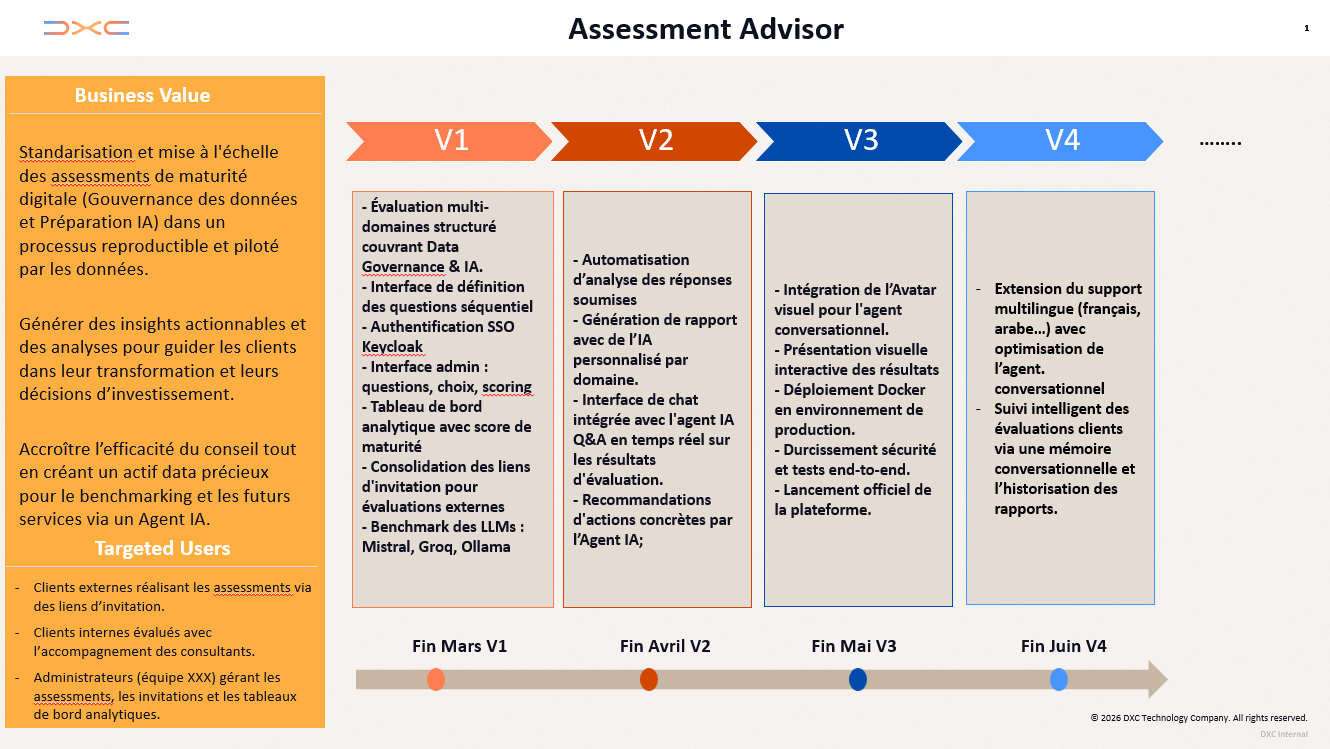
\includegraphics[width=\textwidth]{figures/roadmap.png}
\caption[Feuille de route du projet]{Feuille de route \textit{Assessment Advisor}~: les quatre versions livrées (V1 → V4), la valeur métier attendue, les principales fonctionnalités de chaque palier et les utilisateurs cibles. Document interne DXC ayant servi de cadrage tout au long du projet.}
\label{fig:roadmap}
\end{figure}

\section{Version V1 : Plateforme initiale de \textit{Digital Assessment}}
\textit{Période~: 16 février -- 31 mars 2026.}\\[0.2cm]
La première version livre la plateforme de \textit{Digital Assessment} dans son périmètre nominal, c'est-à-dire l'ensemble fonctionnel qui permet à un client de répondre à une évaluation et à un consultant d'en exploiter les résultats. C'est sur cette base que viendront se greffer, dans les versions suivantes, les fonctions reposant sur l'Agent IA.

\subsection*{Périmètre fonctionnel}
\begin{table}[H]
\centering
\caption{Périmètre fonctionnel de la version V1~: socle applicatif et fonctionnalités cœur livrées au 31 mars 2026.}
\begin{tabularx}{\textwidth}{>{\bfseries}L{4.6cm}Y}
\toprule
Fonctionnalité & Description \\
\midrule
Évaluation multi-domaines & Parcours d'évaluation structuré couvrant la Data Governance et l'AI Readiness, avec sections, questions et choix scorés. \\
Interface de définition séquentielle & Édition des questions une à une par l'administrateur, avec validation à chaque étape. \\
Authentification SSO Keycloak & Connexion fédérée pour les administrateurs et les consultants via OIDC et PKCE. \\
Espace administrateur & Constructeur de référentiel (sections, questions, choix), gestion du scoring et contextes d'évaluation. \\
Tableau de bord analytique & Visualisation du score de maturité, indicateurs globaux, vues par client et par domaine. \\
Support multilingue (FR / EN / AR) & Internationalisation des parcours, des questionnaires et de l'administration, prise en charge du RTL pour l'arabe. \\
Consolidation des invitations externes & Génération et suivi des liens d'invitation, gestion des statuts et des expirations. \\
\textit{Benchmark} LLM & Évaluation préalable de Mistral, Groq et OpenRouter pour orienter le choix des modèles utilisés ensuite par l'Agent IA. \\
\bottomrule
\end{tabularx}
\label{tab:v1}
\end{table}

\subsection*{Réalisation}
Cette première version a posé les fondations techniques de l'application~: la structure Next.js, le socle Spring Boot, la persistance PostgreSQL et l'authentification Keycloak. L'effort principal a porté sur l'industrialisation de trois écrans à forte densité métier~: le constructeur de questionnaires (figure~\ref{fig:builder-screen}), la modale d'édition d'une question (figure~\ref{fig:edit-question-modal}) et le tableau de bord analytique (figure~\ref{fig:analytics-overview}).

La gestion du multilingue a été abordée dès cette version, avec un parcours unique alimenté par des contenus traduits stockés en base sous forme \texttt{JSONB}. Ce choix a évité la duplication d'écrans et permet d'ajouter de nouvelles langues sans modification structurelle du frontend. Le support du RTL pour l'arabe a quant à lui demandé une attention particulière sur les composants analytiques et les modales d'administration.

En parallèle des développements applicatifs, un \textit{benchmark} informel a été conduit sur trois fournisseurs de modèles (Mistral, Groq, OpenRouter) afin d'orienter le choix retenu pour les versions ultérieures. Cette étude préliminaire a confirmé l'intérêt de séparer un modèle «~analytique~» (Mistral) pour la génération structurée et un modèle «~rapide~» (Groq) pour l'assistance conversationnelle.

\begin{figure}[H]
\centering
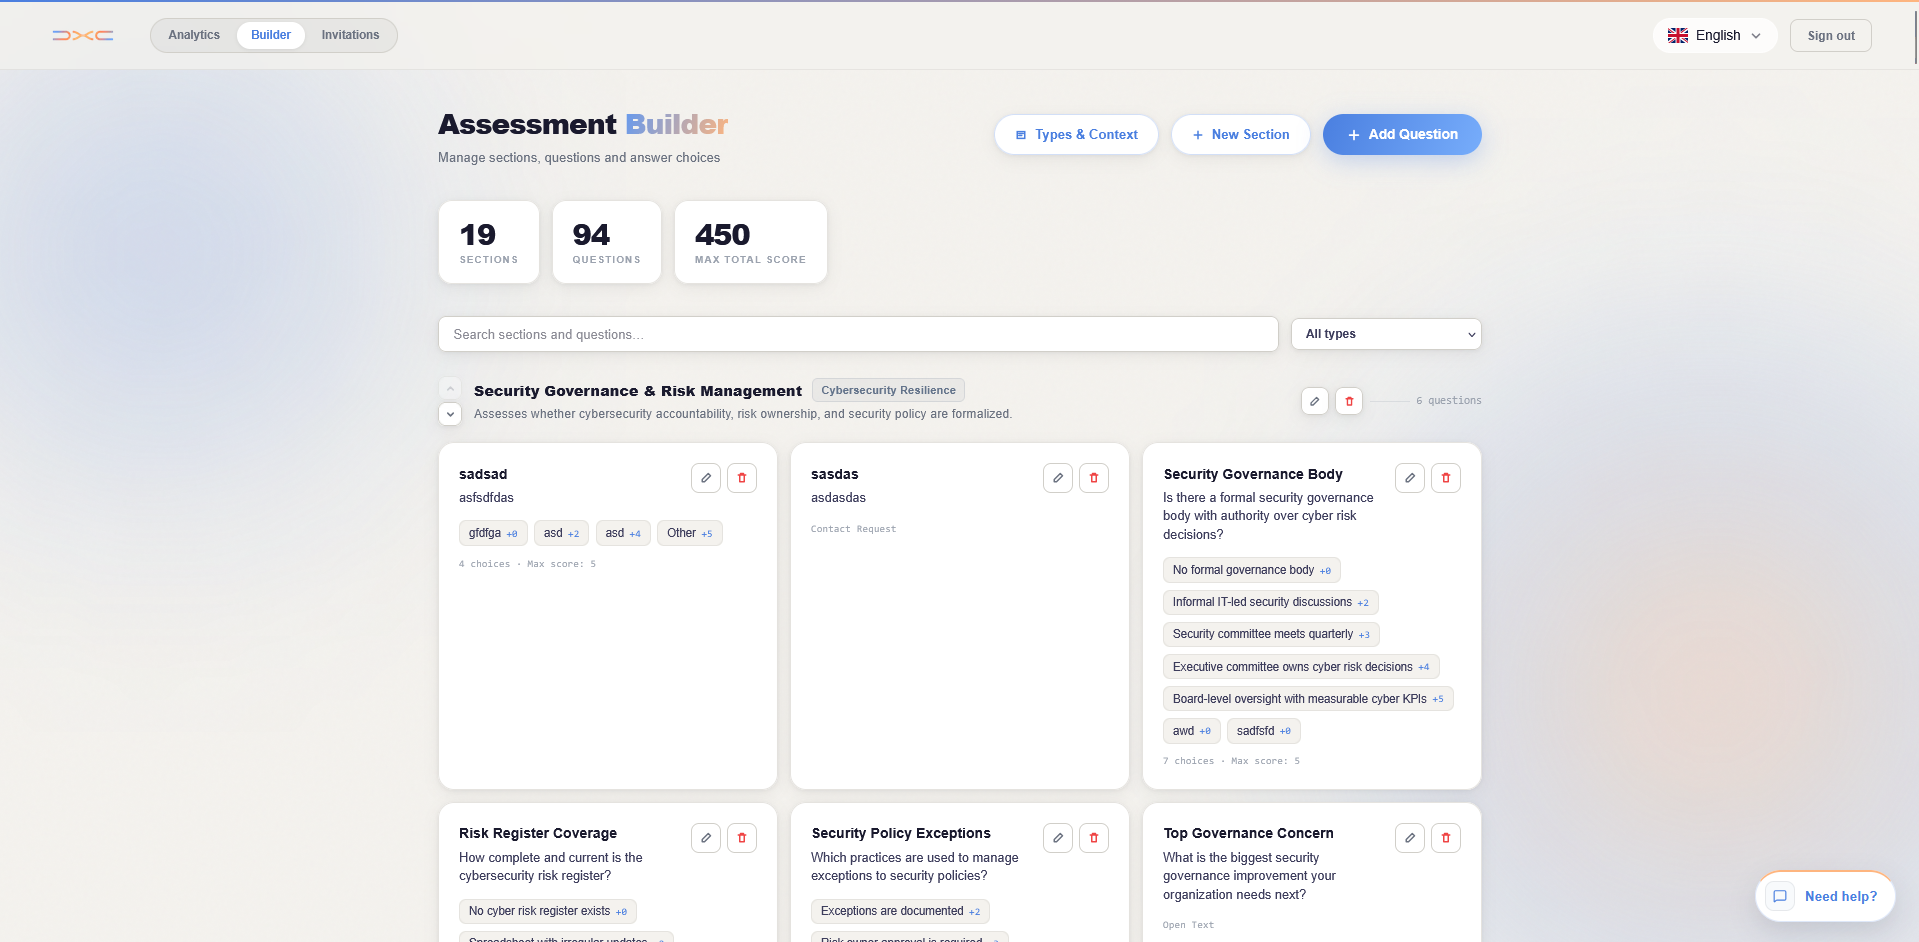
\includegraphics[width=0.95\textwidth]{figures/builder.png}
\caption[Interface du constructeur administrateur]{Interface du constructeur administrateur permettant de consulter les sections, les questions et les scores associés, ainsi que les actions de création, de modification et de suppression sur l'ensemble du référentiel.}
\label{fig:builder-screen}
\end{figure}

\begin{figure}[H]
\centering
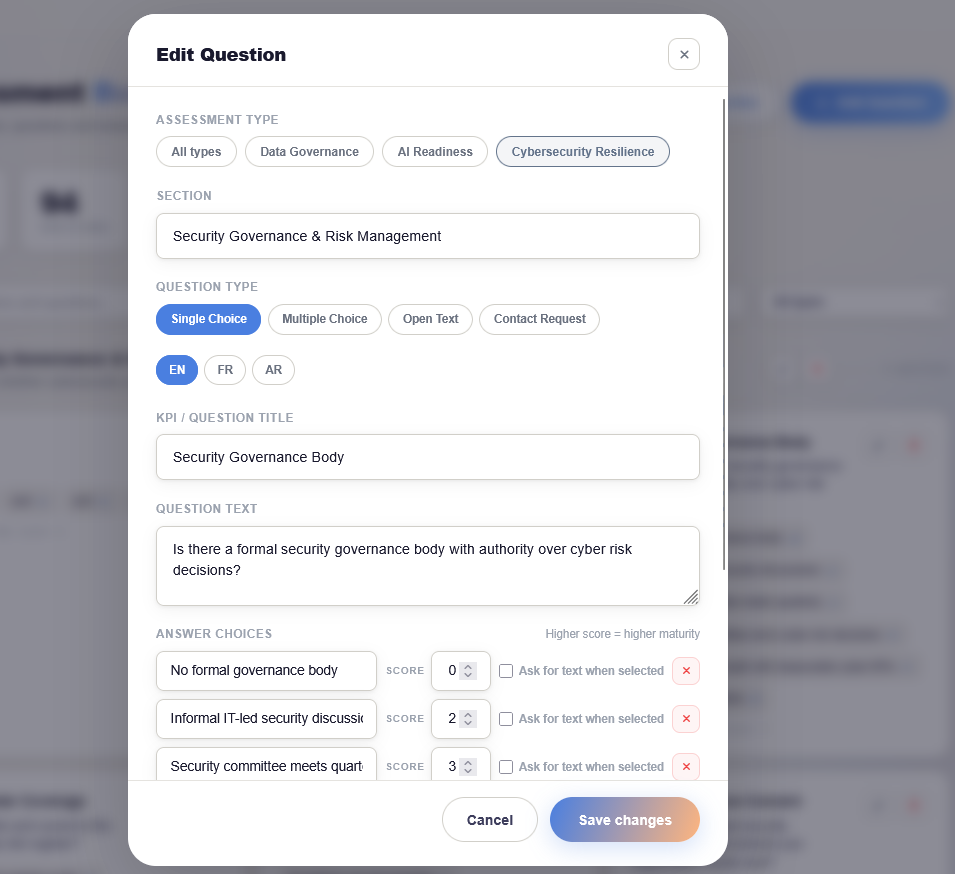
\includegraphics[width=0.62\textwidth]{figures/edit-question-modal.png}
\caption[Fenêtre d'édition d'une question]{Fenêtre modale d'édition d'une question~: l'administrateur y choisit le type d'évaluation, la section, le type de réponse, la langue active et définit les choix de réponse avec leur score, le tout dans une seule interface concentrant les éléments hiérarchiques du référentiel.}
\label{fig:edit-question-modal}
\end{figure}

\begin{figure}[H]
\centering
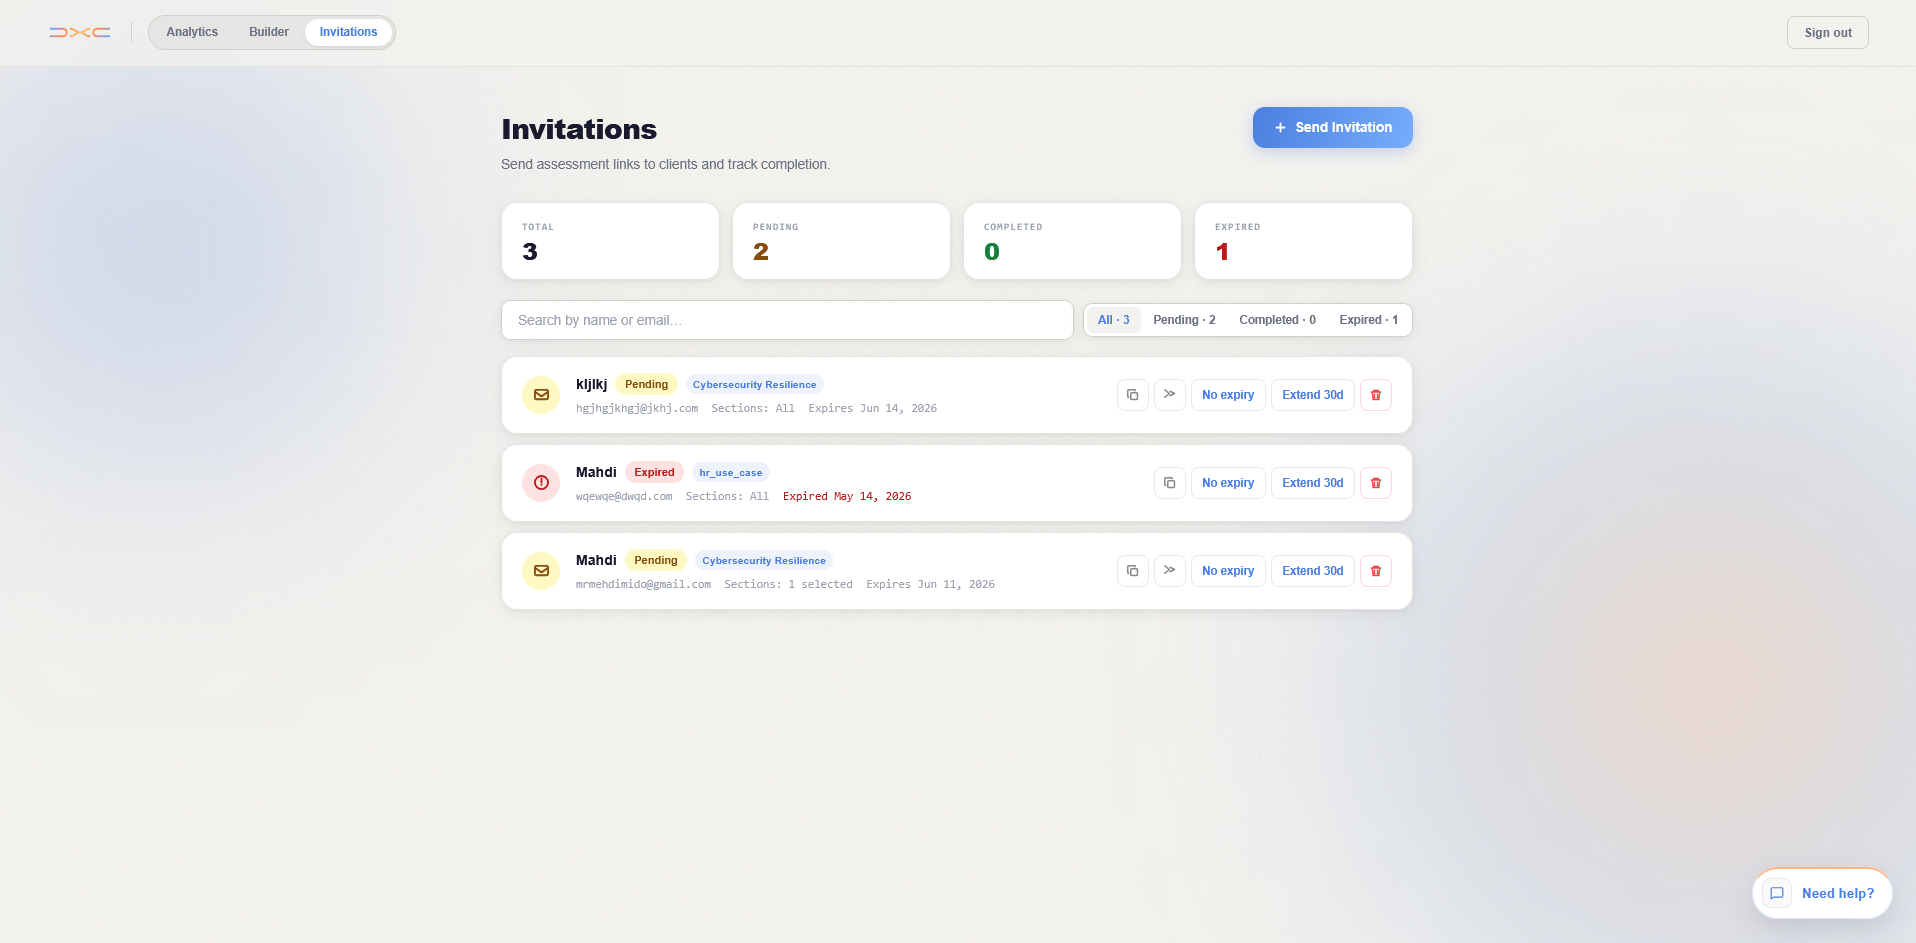
\includegraphics[width=0.95\textwidth]{figures/invitations.png}
\caption[Gestion des invitations]{Interface de gestion des invitations~: indicateurs de suivi (totaux par statut), filtres par état (\textit{pending}, \textit{completed}, \textit{expired}) et actions sur chaque ligne (copie du lien, relance par courriel, prolongation de l'expiration, suppression).}
\label{fig:invitations-screen}
\end{figure}

\begin{figure}[H]
\centering
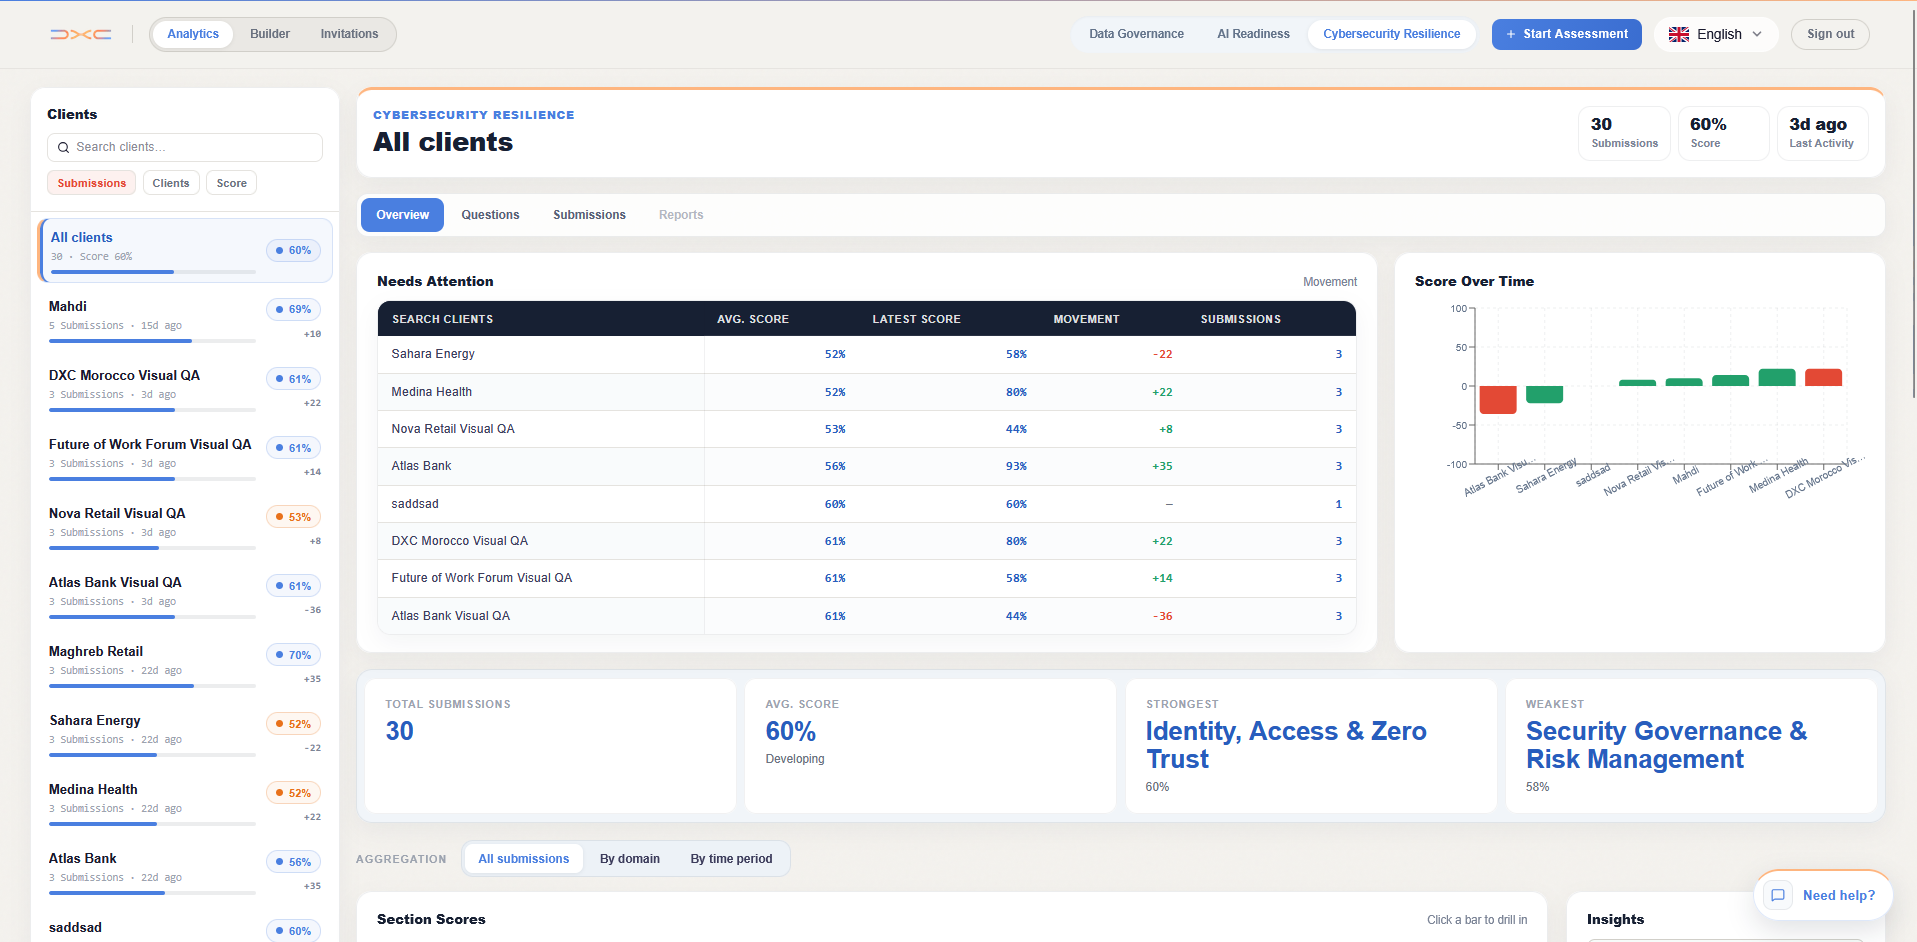
\includegraphics[width=0.95\textwidth]{figures/analytics-overview.png}
\caption[Tableau de bord analytique (V1)]{Tableau de bord analytique de la version V1, agrégeant les clients du portefeuille, les indicateurs globaux de maturité, l'évolution des scores et les vues comparatives par type d'évaluation.}
\label{fig:analytics-overview}
\end{figure}

\subsection*{Livrables de la version}
Le livrable V1 comprend l'application web complète déployée localement via Docker Compose, le constructeur administrateur opérationnel, la gestion des invitations externes, le tableau de bord analytique, les exports CSV et la documentation initiale de l'architecture.

\begin{figure}[H]
\centering
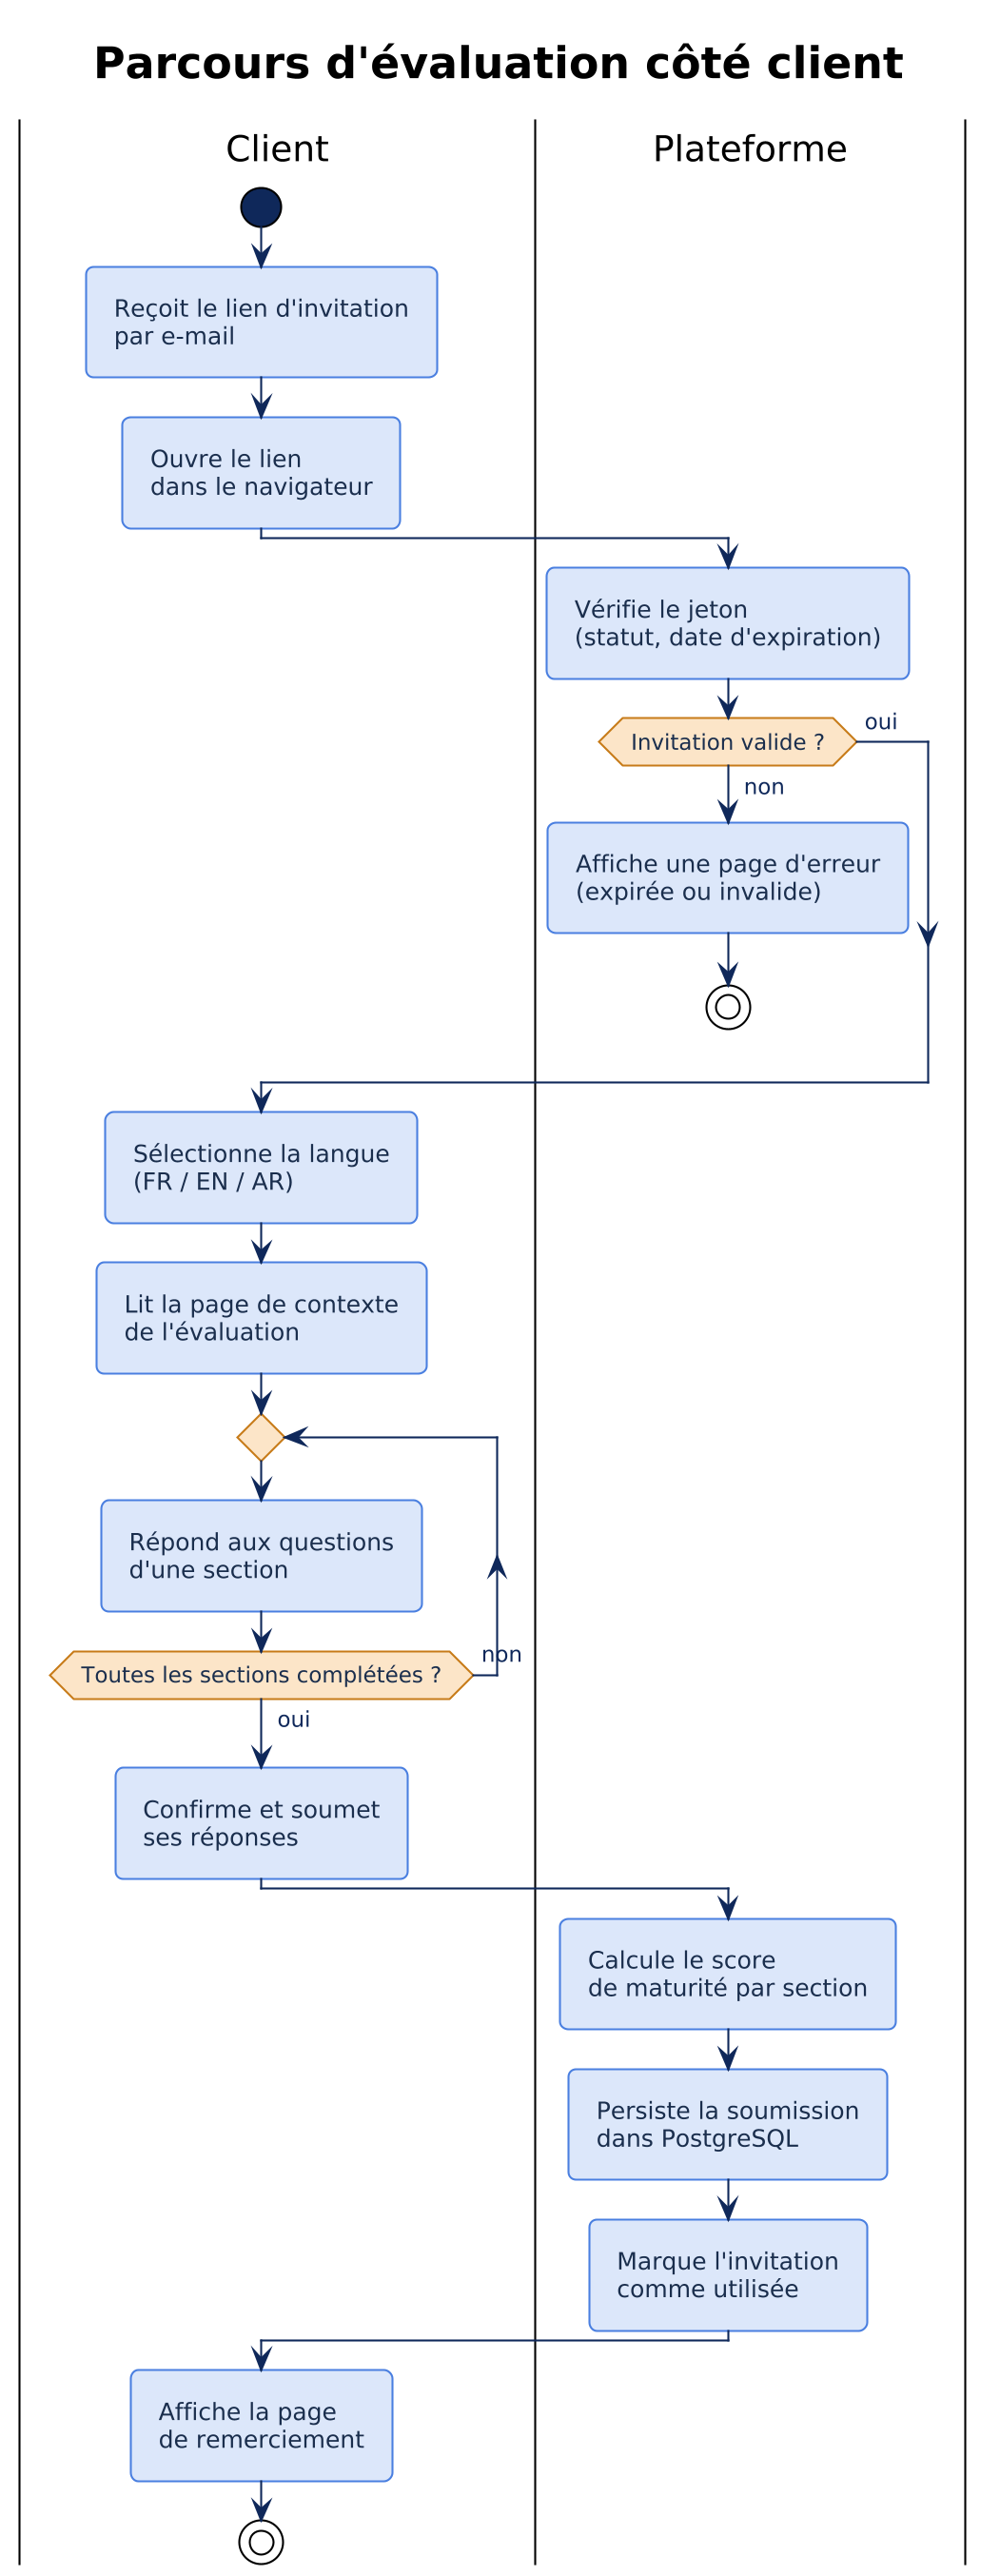
\includegraphics[height=0.78\textheight, keepaspectratio]{figures/uml-activity.png}
\caption[Parcours d'évaluation côté client]{Diagramme d'activité UML décrivant le parcours d'évaluation côté client. Les responsabilités sont réparties en deux couloirs~: le client (ouvre le lien, choisit la langue, répond section par section, confirme) et la plateforme (valide le jeton d'invitation, calcule le score de maturité, persiste la soumission et marque l'invitation comme utilisée). Le branchement conditionnel «~Invitation valide~?~» arrête le parcours si le lien est expiré ou révoqué.}
\end{figure}

\section{Version V2 : Intégration de l'Agent IA dans les flux applicatifs}
\textit{Période~: 1\textsuperscript{er} avril -- 12 mai 2026.}\\[0.2cm]
La deuxième version ouvre la plateforme aux services de l'Agent IA développé en parallèle par Hiba Bouhnin. L'enjeu de cette itération est moins d'ajouter des écrans que de tisser, à plusieurs endroits du produit, les bons points de contact entre les flux applicatifs et les fonctions de génération assistée par modèle de langage.

\subsection*{Périmètre fonctionnel}
\begin{table}[H]
\centering
\caption{Périmètre fonctionnel de la version V2~: intégration des fonctions de l'Agent IA et refonte du tableau de bord analytique.}
\begin{tabularx}{\textwidth}{>{\bfseries}L{4.6cm}Y}
\toprule
Fonctionnalité & Description \\
\midrule
Chatbots client et administrateur & Conversations en \textit{streaming}, réponses contextualisées par domaine ou par évaluation. \\
Contexte administrateur à 3 niveaux & Portée globale, par client ou par domaine, avec un historique conservé indépendamment pour chaque contexte. \\
Recommandations IA & Génération d'analyses par domaine, présentées dans un panneau d'\textit{insights} éditable par le consultant. \\
Rapport PDF narratif & Production automatisée d'un rapport client narratif au format PDF, prêt à être commenté avant partage. \\
Refonte du tableau de bord analytique & Restructuration des sections, hiérarchisation des indicateurs et amélioration du rendu mobile. \\
Réponses IA dans la langue de l'utilisateur & Adaptation des sorties de l'agent au français, à l'anglais ou à l'arabe selon le contexte. \\
\bottomrule
\end{tabularx}
\label{tab:v2}
\end{table}

\subsection*{Réalisation}
L'intégration de l'Agent IA s'est appuyée sur un proxy Next.js qui sert d'unique point d'entrée pour les appels au service FastAPI~: aucun appel direct n'est exposé publiquement. Côté interface, plusieurs surfaces ont été instrumentées pour accueillir l'agent~: un chat client lié au parcours d'évaluation, un chat administrateur capable de basculer entre trois niveaux de contexte, un panneau d'\textit{insights} par domaine avec édition libre, et un module de génération de rapports PDF.

La principale difficulté de cette version a été la gestion des temps de génération, qui peuvent être plus longs qu'un appel REST classique. L'interface a donc été dotée d'états de chargement explicites, de messages d'erreur informatifs et d'une logique de \textit{streaming} permettant à l'utilisateur de voir la réponse s'écrire au fur et à mesure. La refonte du tableau de bord analytique a accompagné ces ajouts, en regroupant les cartes d'indicateurs et en harmonisant les filtres entre les différentes vues.

La vue détaillée d'une soumission (figure~\ref{fig:submissions-screen}) a également été revue pour faciliter l'examen des réponses individuelles, point d'entrée fréquent pour la préparation des rapports IA.

\begin{figure}[H]
\centering
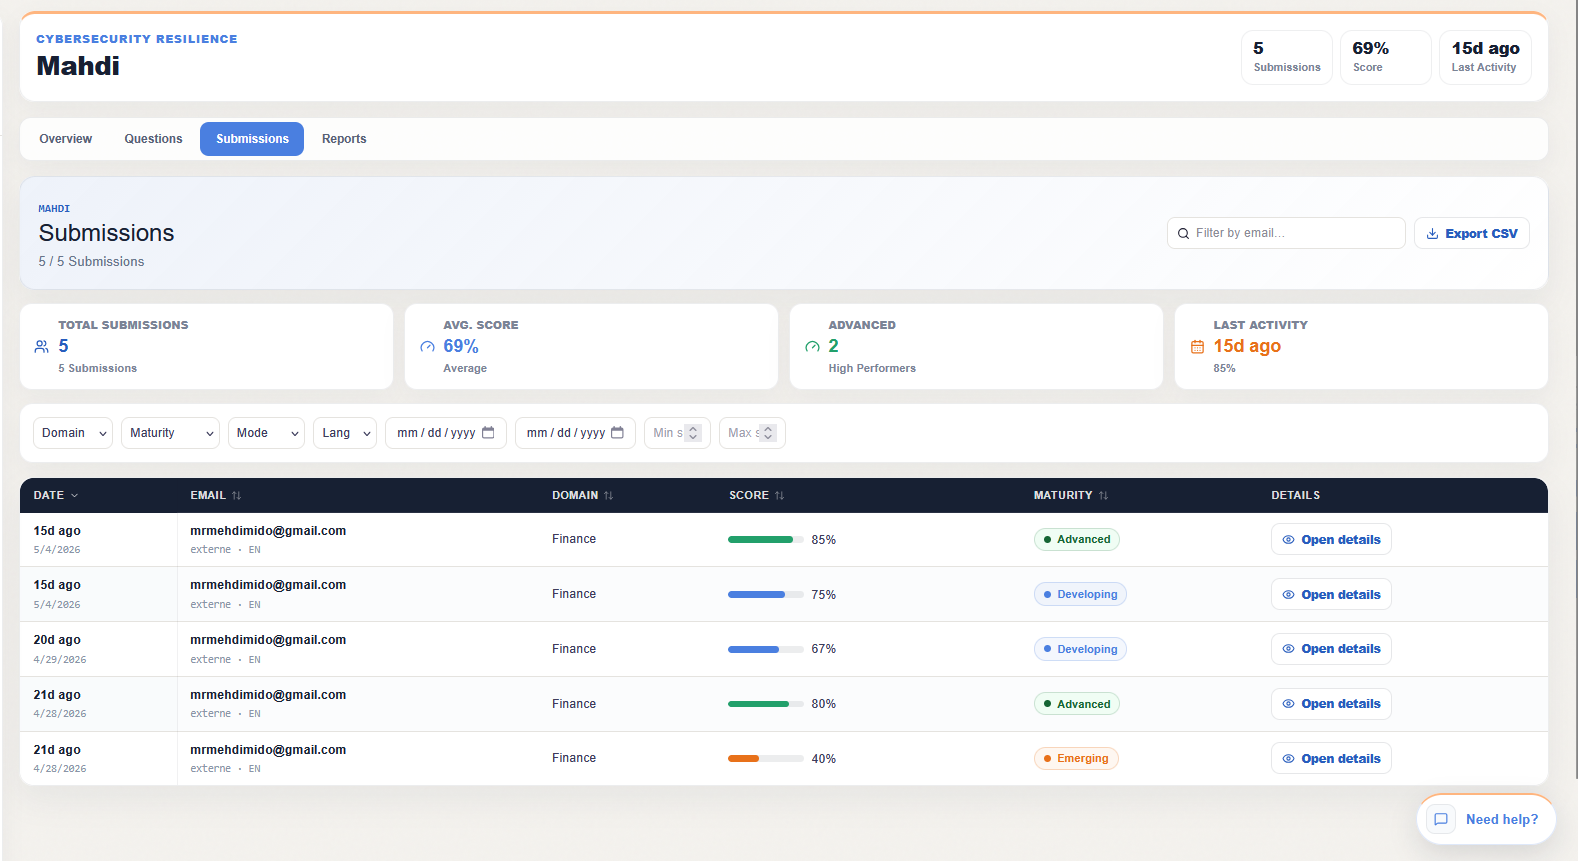
\includegraphics[width=0.95\textwidth]{figures/submissions.png}
\caption[Vue détaillée des soumissions d'un client]{Vue des soumissions d'un client après la refonte du tableau de bord en V2~: indicateurs de synthèse en tête, filtres avancés, export CSV, score de maturité global et accès direct au détail de chaque réponse pour préparation d'un rapport.}
\label{fig:submissions-screen}
\end{figure}

\subsection*{Livrables de la version}
La V2 livre une plateforme dans laquelle l'Agent IA est pleinement intégré aux flux du consultant~: chatbot avec persistance par contexte, recommandations éditables, rapport PDF par client et tableau de bord analytique remanié.

\begin{figure}[H]
\centering
\begin{tikzpicture}[font=\scriptsize, scale=0.92, transform shape,
    component/.style={draw, thick, fill=softblue, align=center,
                      minimum width=3.2cm, minimum height=1.25cm, inner sep=3pt},
    external/.style={draw, thick, dashed, fill=lightgray, align=center,
                     minimum width=3.2cm, minimum height=1.25cm, inner sep=3pt},
    csymbol/.pic={
        \draw[fill=white, thick] (-0.10,-0.08) rectangle (0.10,0.08);
        \draw[fill=white, thick] (-0.10,0.06) rectangle (0.10,0.22);
    },
    link/.style={-Latex, thick},
    lbl/.style={font=\scriptsize\itshape, align=center}]

    \node[component] (ui) {\footnotesize «\,component\,»\\\textbf{Interface frontend}\\\scriptsize Pages analytics et chat};
    \node[component, right=1.4cm of ui] (proxy) {\footnotesize «\,component\,»\\\textbf{Proxy Next.js}\\\scriptsize Routage interne};
    \node[component, right=1.4cm of proxy] (agent) {\footnotesize «\,component\,»\\\textbf{Agent IA — FastAPI}\\\scriptsize Génération, RAG};
    \node[component, below=1.4cm of proxy] (backend) {\footnotesize «\,component\,»\\\textbf{API Spring Boot}\\\scriptsize Soumissions, scores};
    \node[external, below=1.4cm of agent] (models) {\footnotesize «\,external\,»\\\textbf{Mistral} / \textbf{Groq}\\\scriptsize LLM hébergés};

    \foreach \n in {ui,proxy,agent,backend} {
        \pic at ([xshift=-1.35cm, yshift=0.42cm]\n.north) {csymbol};
    }

    \draw[link] (ui) -- node[lbl, above]{HTTPS} (proxy);
    \draw[link] (proxy) -- node[lbl, above]{HTTP interne}
                          node[lbl, below]{Docker network} (agent);
    \draw[link] (agent) -- node[lbl, right]{API LLM\\(HTTPS)} (models);
    \draw[link] (agent) -- node[lbl, sloped, above]{lecture des données} (backend);
\end{tikzpicture}
\caption[Diagramme de composants pour l'intégration de l'Agent IA]{Diagramme de composants UML de l'intégration de l'Agent IA introduite en V2. Le frontend appelle l'agent via un proxy interne Next.js, qui empêche toute exposition publique du service. L'agent récupère les données nécessaires auprès du backend Spring Boot et délègue la génération aux modèles externes Mistral et Groq, représentés en pointillés pour indiquer leur statut de composant externe.}
\end{figure}

\section{Version V3 : Copilote « Build with AI » et préparation au déploiement}
\textit{Période~: 13 mai -- 31 mai 2026.}\\[0.2cm]
La troisième version élargit le rôle de l'Agent IA en l'introduisant dans le poste de travail du consultant lui-même, à travers un copilote d'aide à la construction des questionnaires. Elle prépare également la solution à une mise en production, en consolidant le périmètre de sécurité et en couvrant le code par une suite de tests automatisés.

\subsection*{Périmètre fonctionnel}
\begin{table}[H]
\centering
\caption{Périmètre fonctionnel de la version V3~: copilote d'administration, sécurisation et industrialisation.}
\begin{tabularx}{\textwidth}{>{\bfseries}L{4.6cm}Y}
\toprule
Fonctionnalité & Description \\
\midrule
Copilote « Build with AI » & Assistance par IA dans le constructeur de questionnaires~: génération de sections, de questions et de choix à partir d'une brève description. \\
Avatar visuel de l'assistant & Identité graphique du chat assistant, présence visuelle dans les écrans concernés. \\
Portée client pour le consultant & Restriction des accès analytics, chat et rapports au périmètre du consultant connecté. \\
Déploiement \textit{production-ready} & Mise en service de la plateforme derrière l'application web, l'Agent IA n'étant accessible qu'au travers du proxy. \\
Suite de tests étendue & Couverture des modules frontend, backend et agent par des tests unitaires et d'intégration. \\
\bottomrule
\end{tabularx}
\label{tab:v3}
\end{table}

\subsection*{Réalisation}
Le copilote « Build with AI » est l'évolution la plus visible de cette version~: il permet à un administrateur de partir d'une description en langage naturel pour générer une première trame de questionnaire que l'utilisateur affine ensuite. Cette assistance a demandé d'aligner les contrats de données entre le constructeur, l'Agent IA et le backend, pour que les éléments générés soient directement utilisables par les écrans d'administration.

La sécurisation de la solution a été un autre chantier important. Côté \textit{scoping}, le périmètre de consultation a été restreint au consultant connecté~: il ne voit désormais que les clients dont il a la responsabilité, sur l'ensemble des modules (analytics, chat, rapports). Côté déploiement, l'Agent IA a été placé derrière l'application web, sur le réseau Docker interne, et n'est joignable qu'à travers le proxy Next.js. Enfin, une suite de tests a été constituée pour le frontend (116 assertions \texttt{node:assert}), le backend (49 tests JUnit) et l'agent, afin d'éviter les régressions au fil des évolutions à venir.

\subsection*{Livrables de la version}
À l'issue de la V3, la plateforme dispose d'un copilote de construction de questionnaires, d'une expérience de chat dotée d'un avatar dédié, d'un cloisonnement par consultant et d'un environnement de déploiement adapté à un usage opérationnel, couvert par une suite de tests automatisés.

\section{Version V4 : Couverture multilingue de l'IA et édition des brouillons}
\textit{Période~: 1\textsuperscript{er} juin -- 16 juin 2026.}\\[0.2cm]
La dernière version consolide l'expérience multilingue de l'Agent IA, déjà amorcée en V2, et introduit un mécanisme d'édition des contenus produits par l'agent. L'objectif est de garantir que les sorties générées restent maîtrisées par le consultant et préservent le sens même lorsque la conversation bascule d'une langue à l'autre.

\subsection*{Périmètre fonctionnel}
\begin{table}[H]
\centering
\caption{Périmètre fonctionnel de la version V4~: multilinguisme bout en bout pour l'IA et édition contrôlée des brouillons.}
\begin{tabularx}{\textwidth}{>{\bfseries}L{4.6cm}Y}
\toprule
Fonctionnalité & Description \\
\midrule
Couverture multilingue de l'IA & Prise en charge complète des trois langues sur tous les modes de chat et toutes les natures de réponses. \\
Conservation de contexte au changement de langue & Le contexte conversationnel est préservé lorsque l'utilisateur bascule de langue en milieu d'échange. \\
Historique de chat à trois niveaux & Persistance durable des conversations, même en cas de redémarrage de l'agent. \\
Brouillons IA éditables & Édition libre des contenus générés par l'agent, avec historique complet et possibilité de retour en arrière. \\
\bottomrule
\end{tabularx}
\label{tab:v4}
\end{table}

\subsection*{Réalisation}
Le multilinguisme de l'Agent IA a été repris bout en bout pour couvrir tous les modes de chat et tous les types de réponses. Une particularité importante a été la gestion du changement de langue en milieu de conversation~: plutôt que d'effacer le contexte, le système conserve l'historique précédent et adapte uniquement la langue des réponses suivantes, ce qui évite à l'utilisateur de devoir reformuler ses demandes.

L'historique des conversations a été rendu durable sur les trois niveaux de contexte introduits en V2 (global, client, domaine), de sorte qu'un redémarrage de l'agent ne provoque plus la perte des échanges en cours. Les brouillons produits par l'agent, qu'il s'agisse de recommandations ou de rapports, sont devenus éditables côté interface, avec un historique des modifications permettant d'annuler un changement et de revenir à une version précédente.

\subsection*{Livrables de la version}
La V4 finalise la plateforme avec une couverture multilingue intégrale de l'Agent IA, une mémoire conversationnelle durable et un mécanisme d'édition contrôlée des contenus générés. La solution atteint ainsi l'ensemble du périmètre fonctionnel attendu pour la défense du projet.

\begin{figure}[H]
\centering
\begin{tikzpicture}[font=\small,
    box/.style={draw, rounded corners, fill=softblue, align=center,
                minimum width=3.0cm, minimum height=0.9cm},
    decision/.style={diamond, draw, fill=lightgray, aspect=2.2, align=center,
                     inner sep=1pt, minimum height=0.8cm},
    startnode/.style={circle, fill=black, minimum size=0.4cm, inner sep=0},
    endnode/.style={circle, draw, fill=white, minimum size=0.55cm, inner sep=0,
                    label={[font=\Large]center:$\bullet$}},
    arr/.style={-Latex, thick}]

    \node[startnode] (start) at (0,0) {};
    \node[box, right=0.6cm of start] (unit) {Tests\\unitaires};
    \node[box, right=0.6cm of unit] (ui) {Vérifications\\visuelles};
    \node[box, right=0.6cm of ui] (resp) {Contrôles\\responsive};
    \node[decision, right=0.7cm of resp] (ok) {Régressions~?};
    \node[box, below=1.0cm of ok] (fix) {Corrections};
    \node[endnode, above right=0.4cm and 0.7cm of ok] (end) {};

    \draw[arr] (start) -- (unit);
    \draw[arr] (unit) -- (ui);
    \draw[arr] (ui) -- (resp);
    \draw[arr] (resp) -- (ok);
    \draw[arr] (ok) -- node[above, font=\scriptsize]{[non]} (end);
    \draw[arr] (ok) -- node[right, font=\scriptsize]{[oui]} (fix);
    \draw[arr] (fix.west) -| node[below, pos=0.25, font=\scriptsize]{itération} (unit.south);
\end{tikzpicture}
\caption[Diagramme d'activité de la finalisation]{Diagramme d'activité UML du processus de finalisation V4~: enchaînement des tests unitaires, des vérifications visuelles et des contrôles responsive, suivi d'un nœud de décision qui reboucle vers les tests tant que des régressions subsistent.}
\end{figure}

\section*{Bilan de réalisation}
Au terme des quatre versions, la plateforme couvre le parcours métier visé~: préparation du questionnaire, invitation du client, réponse à l'évaluation, consultation des résultats, export des données et intégration des services IA. Chaque module manipule des données structurées, s'appuie sur des services backend testés et reprend le cycle d'évaluation modélisé au chapitre~3.

Le contenu utilisé pour la démonstration n'est volontairement pas minimal. Le référentiel administré couvre plusieurs sections, plusieurs dizaines de questions et leurs choix associés. Cette volumétrie a permis de vérifier que les interfaces, en particulier le constructeur et le tableau de bord analytique, restent lisibles sur un cas réaliste et pas seulement sur le scénario «~deux questions, trois clients~» qui rend toute interface agréable.

\begin{table}[H]
\centering
\caption{Bilan fonctionnel des modules réalisés.}
\begin{tabularx}{\textwidth}{>{\bfseries}L{4cm}Y}
\toprule
Module & Résultat obtenu \\
\midrule
Accueil et parcours publics & Accès aux évaluations, sélection du type d'évaluation, choix de langue et orientation vers le mode de réponse adapté. \\
Questionnaire & Chargement dynamique des sections et questions, progression, confirmation et soumission des réponses. \\
Constructeur administrateur & Consultation, création et modification des sections, questions, choix, scores et contenus multilingues, avec services d'administration associés. \\
Invitations & Création, suivi, copie de lien, relance, expiration, endpoints métier et distinction entre mode interne et mode externe. \\
Analyse & Indicateurs globaux, vues client, filtres, graphiques, détail des soumissions, agrégations backend et export CSV. \\
Agent IA intégré & Génération de rapports, recommandations, assistance conversationnelle et affichage des états associés. \\
\bottomrule
\end{tabularx}
\end{table}

\section*{Difficultés rencontrées et solutions adoptées}
Aucun projet d'application métier ne se déroule selon le plan initial, et celui-ci n'y a pas fait exception. Les difficultés rencontrées concernaient moins l'ajout de fonctionnalités prises individuellement que le maintien d'une cohérence d'ensemble malgré la diversité des parcours, des langues, des profils utilisateurs et des volumes de données à présenter.

La gestion du multilingue, en particulier l'arabe avec son affichage de droite à gauche, a été l'un des premiers points sensibles. Le choix initial de dupliquer les écrans aurait simplifié l'implémentation mais multiplié la dette de maintenance. La solution retenue passe par une centralisation des contenus traduits et une bascule contextuelle de la direction d'affichage~; elle conserve un parcours unique tout en adaptant naturellement l'expérience à chaque langue.

Le constructeur administrateur a également demandé plusieurs itérations. Les données manipulées y sont profondément hiérarchiques (types d'évaluation, sections, questions, choix, traductions) et peuvent devenir volumineuses dès qu'un référentiel atteint une taille réaliste. Pour éviter qu'une interface unique ne devienne illisible, l'édition a été organisée en cartes, modales et groupes de sections, de sorte qu'une action reste toujours localisée au niveau hiérarchique pertinent et limite le risque d'erreur.

Les tableaux de bord ont posé un problème de nature différente, plus ergonomique que technique~: comment offrir suffisamment de détail à un consultant sans produire un écran indigeste sur un format tablette ou mobile~? La réponse, plutôt itérative, a combiné corrections responsive, hiérarchisation visuelle des cartes d'indicateurs, filtres regroupés et vues par onglets, jusqu'à parvenir à un compromis acceptable entre densité d'information et lisibilité.

L'intégration du module IA a soulevé une contrainte spécifique~: les appels de génération peuvent être plusieurs fois plus longs qu'une requête backend classique, et leurs réponses ne doivent pas être prises pour argent comptant. L'interface intègre donc des états de chargement explicites, des messages d'erreur informatifs, des garde-fous de contexte pour l'assistant administrateur, et une logique où les contenus produits par l'Agent IA viennent en appui du consultant sans court-circuiter sa validation.

\begin{table}[H]
\centering
\caption{Principales difficultés rencontrées et réponses apportées.}
\begin{tabularx}{\textwidth}{>{\bfseries}L{4cm}Y}
\toprule
Difficulté & Solution adoptée \\
\midrule
Multilingue et RTL & Centralisation du contexte de langue, adaptation de la direction d'affichage et conservation d'un parcours unique. \\
Questionnaires configurables & Structuration des contenus en types, sections, questions, choix et traductions, avec édition depuis l'espace administrateur. \\
Lisibilité analytique & Utilisation de cartes d'indicateurs, filtres, onglets, tableaux et vues détaillées pour organiser les résultats. \\
Responsive design & Corrections des débordements, adaptation des tableaux, ajustement des espacements et vérification des écrans critiques. \\
Intégration IA & États de chargement, gestion des erreurs, proxy Next.js et limitation du périmètre de l'assistant selon le contexte. \\
\bottomrule
\end{tabularx}
\end{table}

\section*{Validation de la solution}
La validation de la solution s'est faite à la fin de chaque version, puis lors de la phase de finalisation en V4. Les vérifications ont porté sur les parcours essentiels~: accès aux évaluations, soumission des réponses, gestion des invitations, modification des questions, consultation des tableaux de bord, export des soumissions et intégration des services IA. Ce contrôle régulier a aidé à détecter les régressions au moment où de nouveaux modules étaient ajoutés.

Les contrôles frontend ont été complétés par des tests ciblés sur certaines fonctions de traitement de données, notamment les agrégations, l'export CSV, le formatage des réponses et le chargement des rapports. Les parcours ont aussi été vérifiés avec plusieurs profils d'utilisation afin de confirmer que les actions administrateur restent protégées et que les vues client ne donnent accès qu'aux informations nécessaires.

Les cas limites visibles côté interface ont également été vérifiés~: absence de données, erreurs d'appel API, délai de génération des rapports IA, invitation expirée, contenu multilingue incomplet et affichage sur petit écran. Ces vérifications ont contribué à améliorer la robustesse perçue de la plateforme, même lorsque tous les services ne répondent pas dans des conditions idéales.

\paragraph{Synthèse quantitative des tests.}
\begin{table}[H]
\centering
\caption{Synthèse quantitative des tests automatisés et des vérifications manuelles réalisés sur la plateforme.}
\begin{tabularx}{\textwidth}{>{\bfseries}L{4.5cm}L{2.4cm}Y}
\toprule
Périmètre & Volume & Outillage et portée \\
\midrule
Tests unitaires backend & 49 cas (13 classes) & JUnit 5 et Mockito sur les services métier (InvitationService, SubmissionService, AssessmentService, AdminCrudService, AnalyticsRows, AnalyticsMath, AssessmentTypeService, DomainService), la sécurité (AuthScopeService), la gestion des exceptions (GlobalExceptionHandler), la configuration (DataSeeder) et le modèle de domaine (Choice, PerformanceIndex). \\
Tests unitaires frontend & 13 modules, 116 assertions & Tests basés sur \texttt{node:assert} couvrant les agrégations analytiques, la construction des questionnaires, le rendu des réponses, l'export CSV, la persistance des brouillons de rapport, la gestion d'état d'URL, les filtres d'invitations et les utilitaires de stockage navigateur. \\
Tests fonctionnels manuels & 7 scénarios principaux & Parcours client multilingue, ouverture d'invitation, administration du référentiel, exploration analytique, génération de rapport IA, assistance conversationnelle et déconnexion. \\
Vérifications responsive & 3 résolutions cibles & Affichage mobile 360\,px, tablette 768\,px, desktop 1440\,px sur les écrans accueil, évaluation, administration et tableau de bord. \\
Audits qualité interface & Lighthouse & Audits de performance, d'accessibilité, de bonnes pratiques et de SEO sur la page d'accueil et le tableau de bord. \\
\bottomrule
\end{tabularx}
\label{tab:tests-synthese}
\end{table}

\begin{figure}[H]
\centering
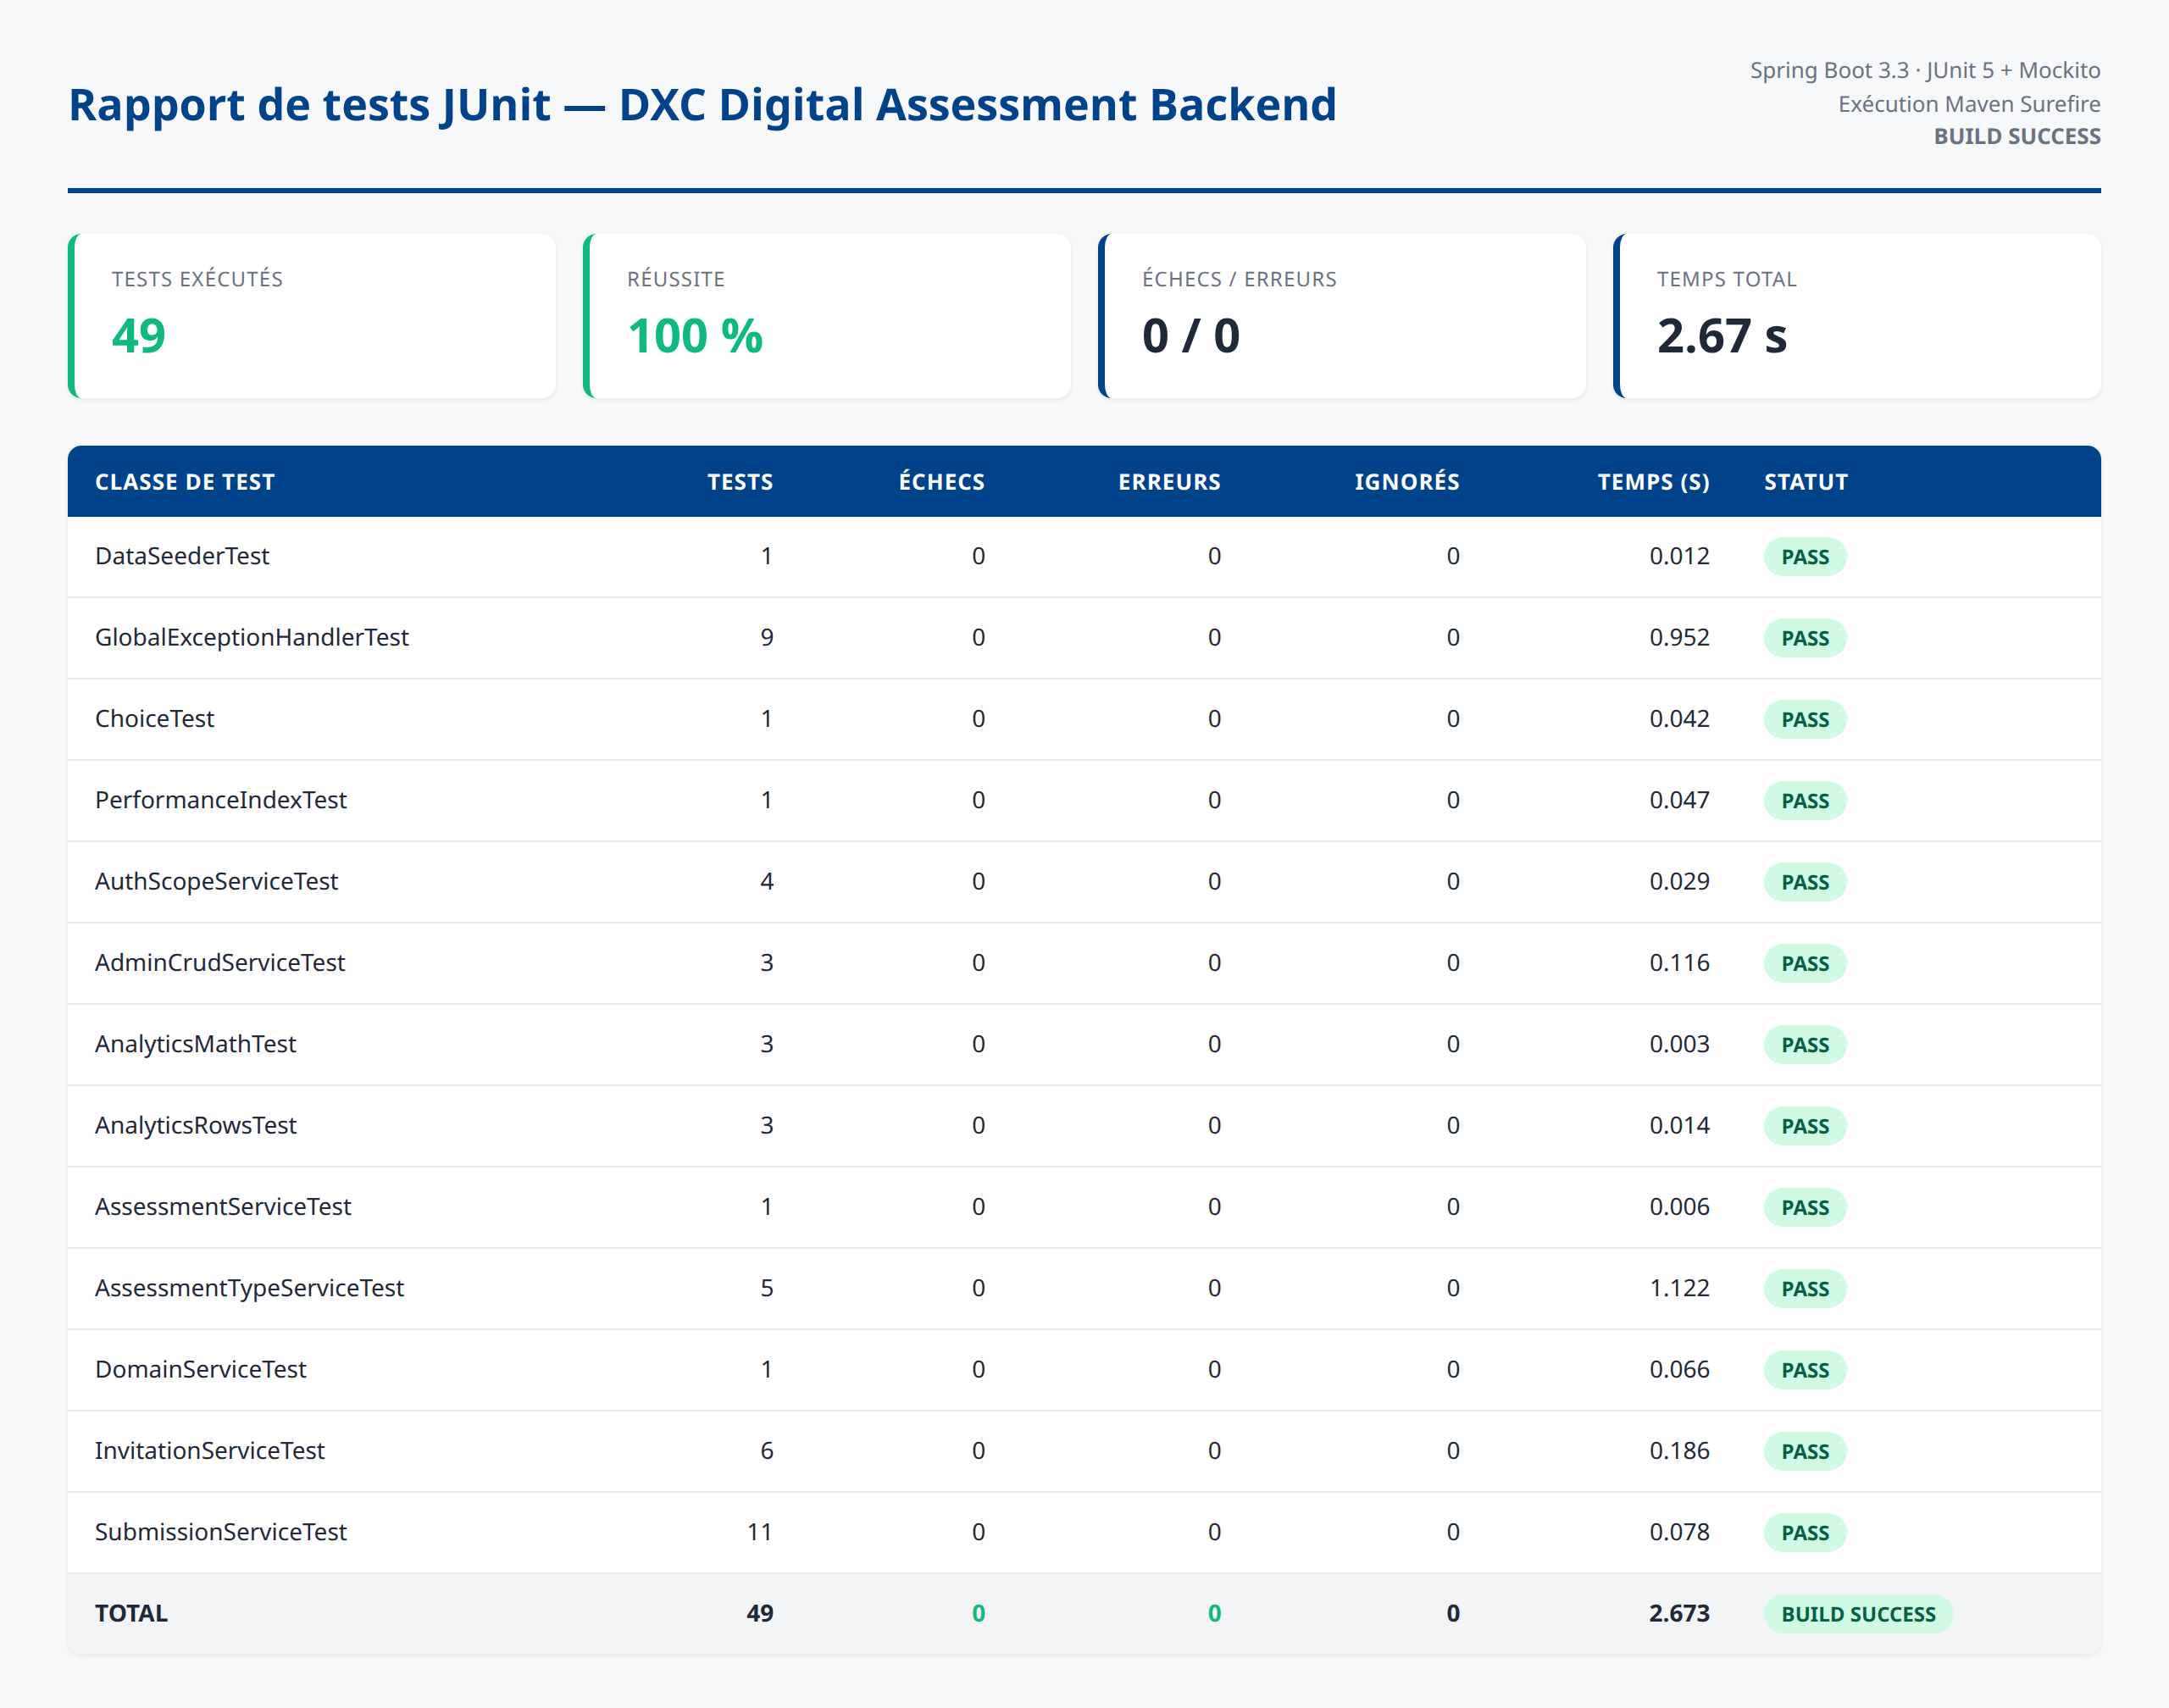
\includegraphics[width=0.92\textwidth]{figures/test-junit-report.png}
\caption[Rapport JUnit du backend Spring Boot]{Rapport agrégé des tests JUnit du backend Spring Boot, généré à partir des sorties Maven Surefire~: 49~tests répartis sur 13~classes (services métier, sécurité, modèles, gestion des exceptions) exécutés en 2,67~secondes avec un taux de réussite de 100\,\%.}
\label{fig:junit-report}
\end{figure}

\begin{figure}[H]
\centering
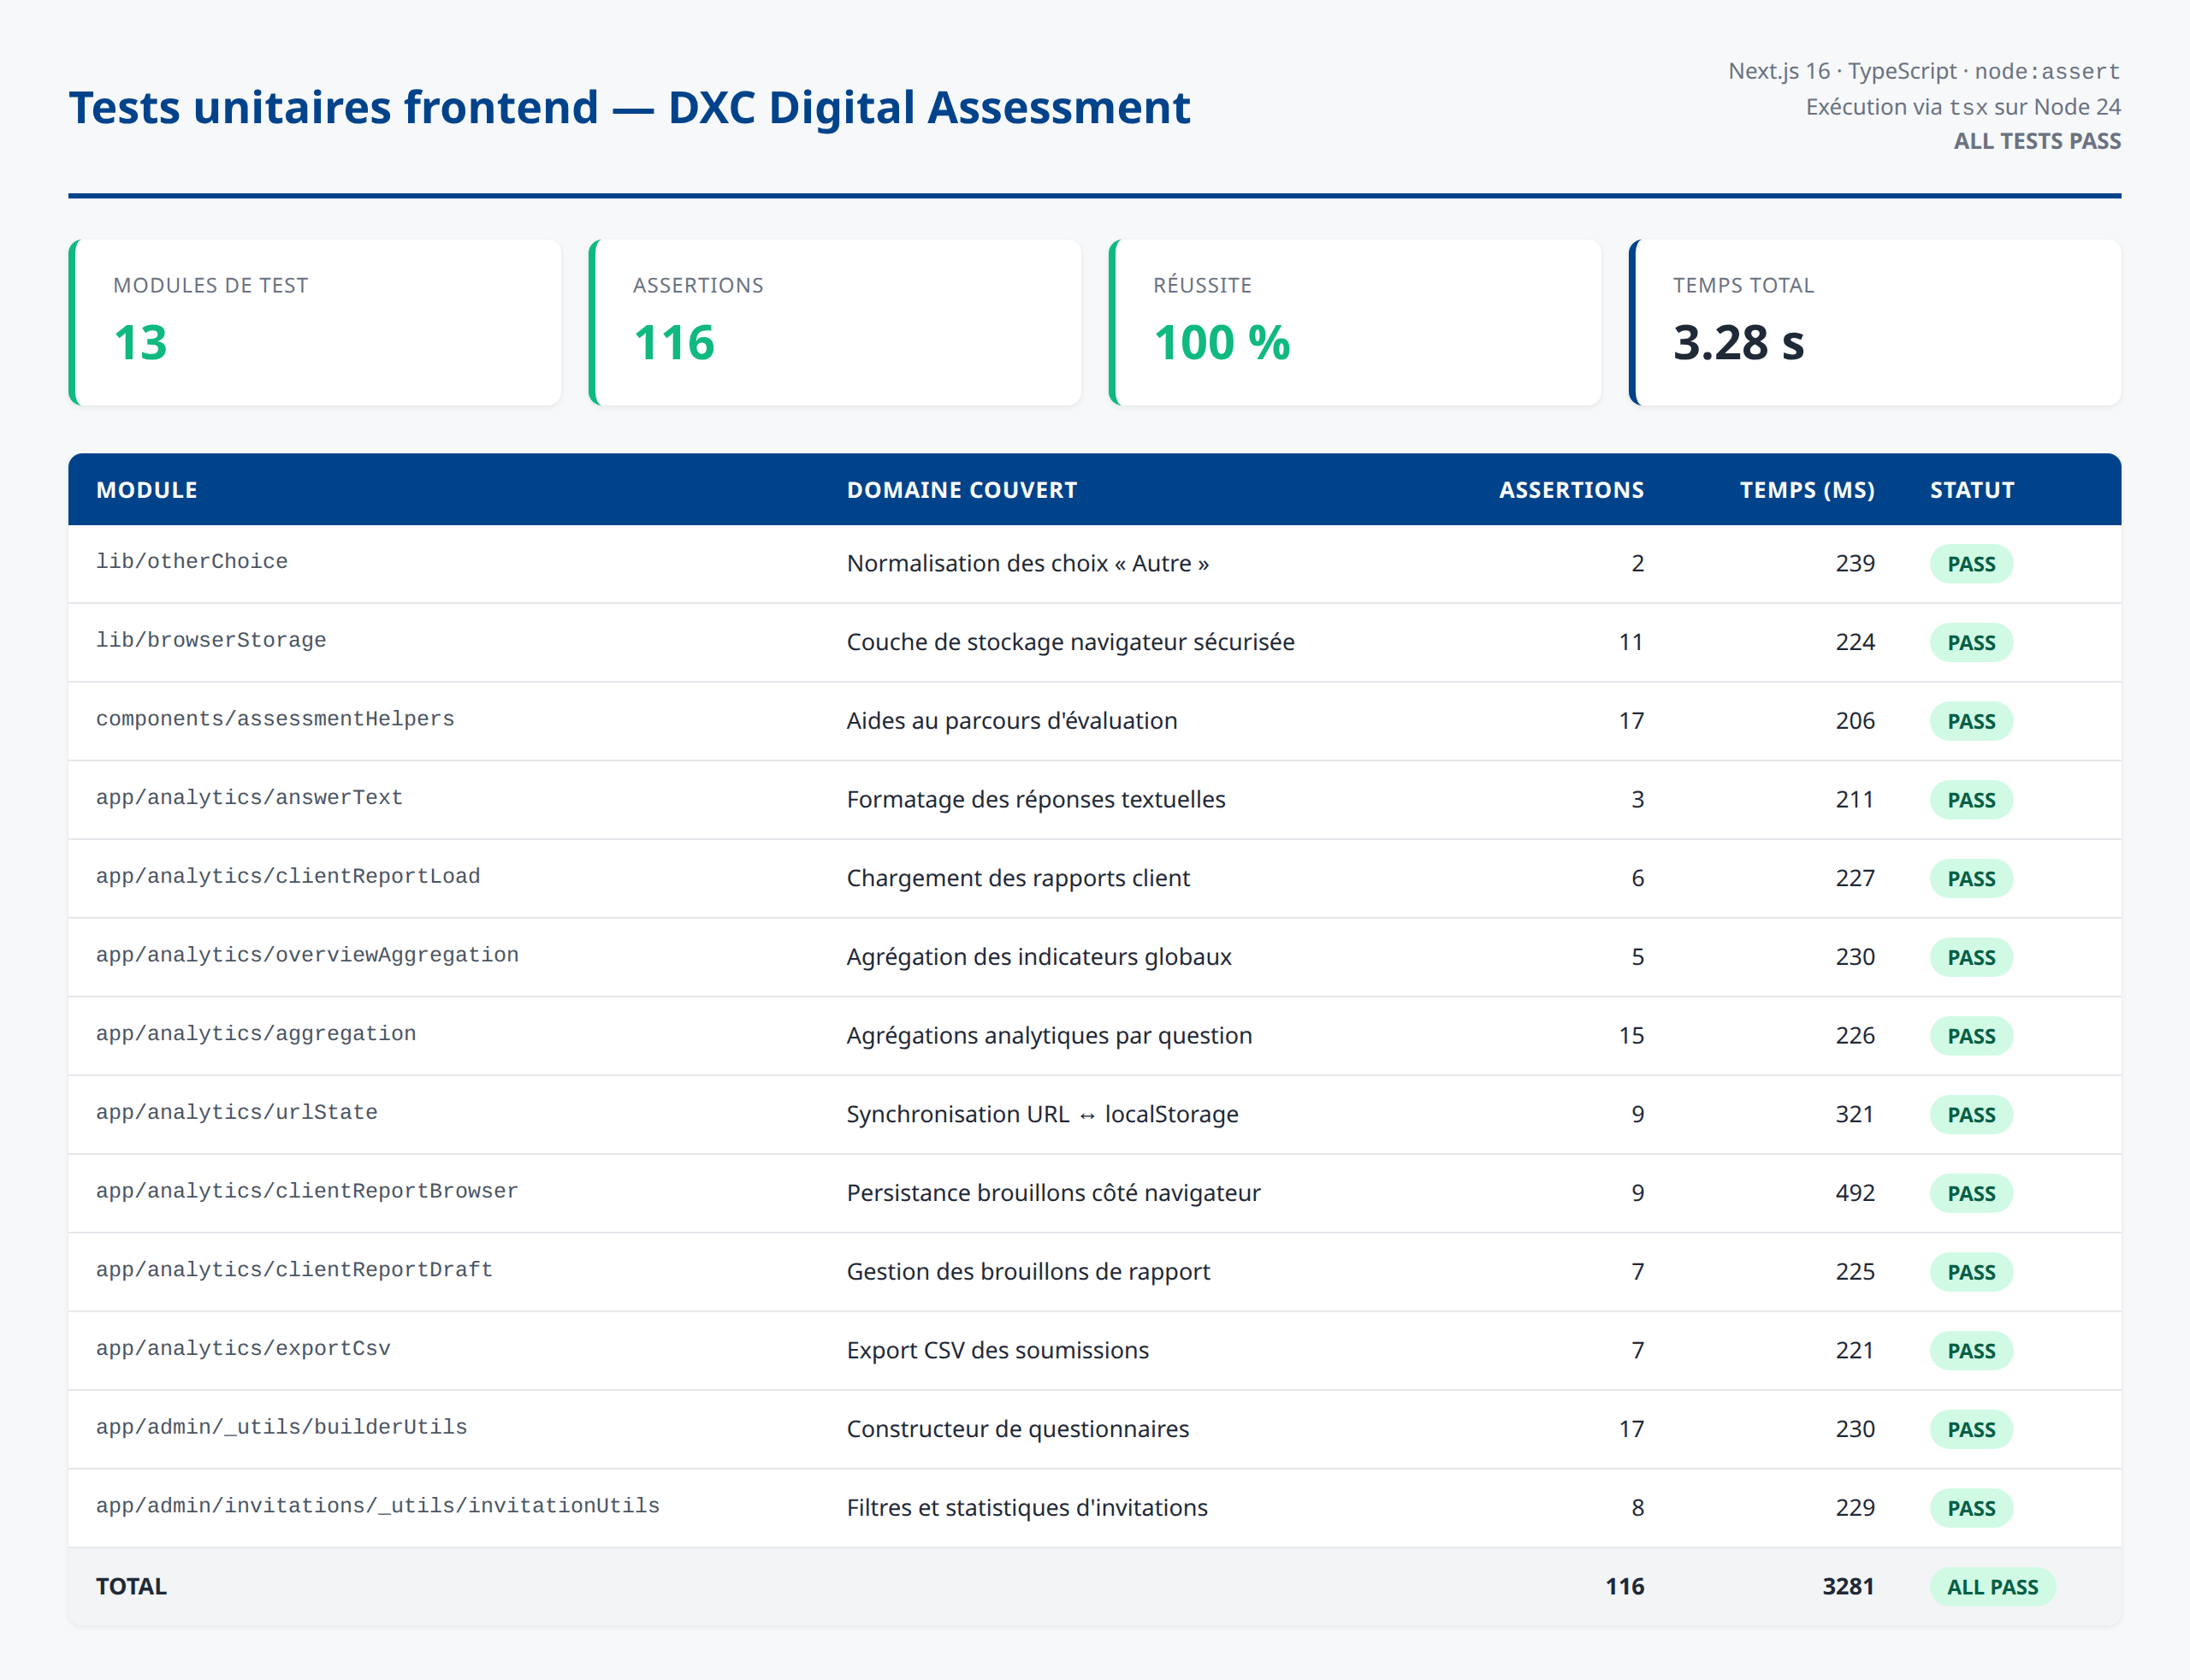
\includegraphics[width=0.92\textwidth]{figures/test-frontend-report.png}
\caption[Tests unitaires du frontend Next.js]{Résultat de l'exécution des tests unitaires du frontend~: 13~modules de test couvrant les agrégations analytiques, l'export CSV, la persistance des brouillons de rapport, la synchronisation URL/localStorage et les utilitaires d'administration, totalisant 116~assertions toutes vertes.}
\label{fig:frontend-report}
\end{figure}

\begin{figure}[H]
\centering
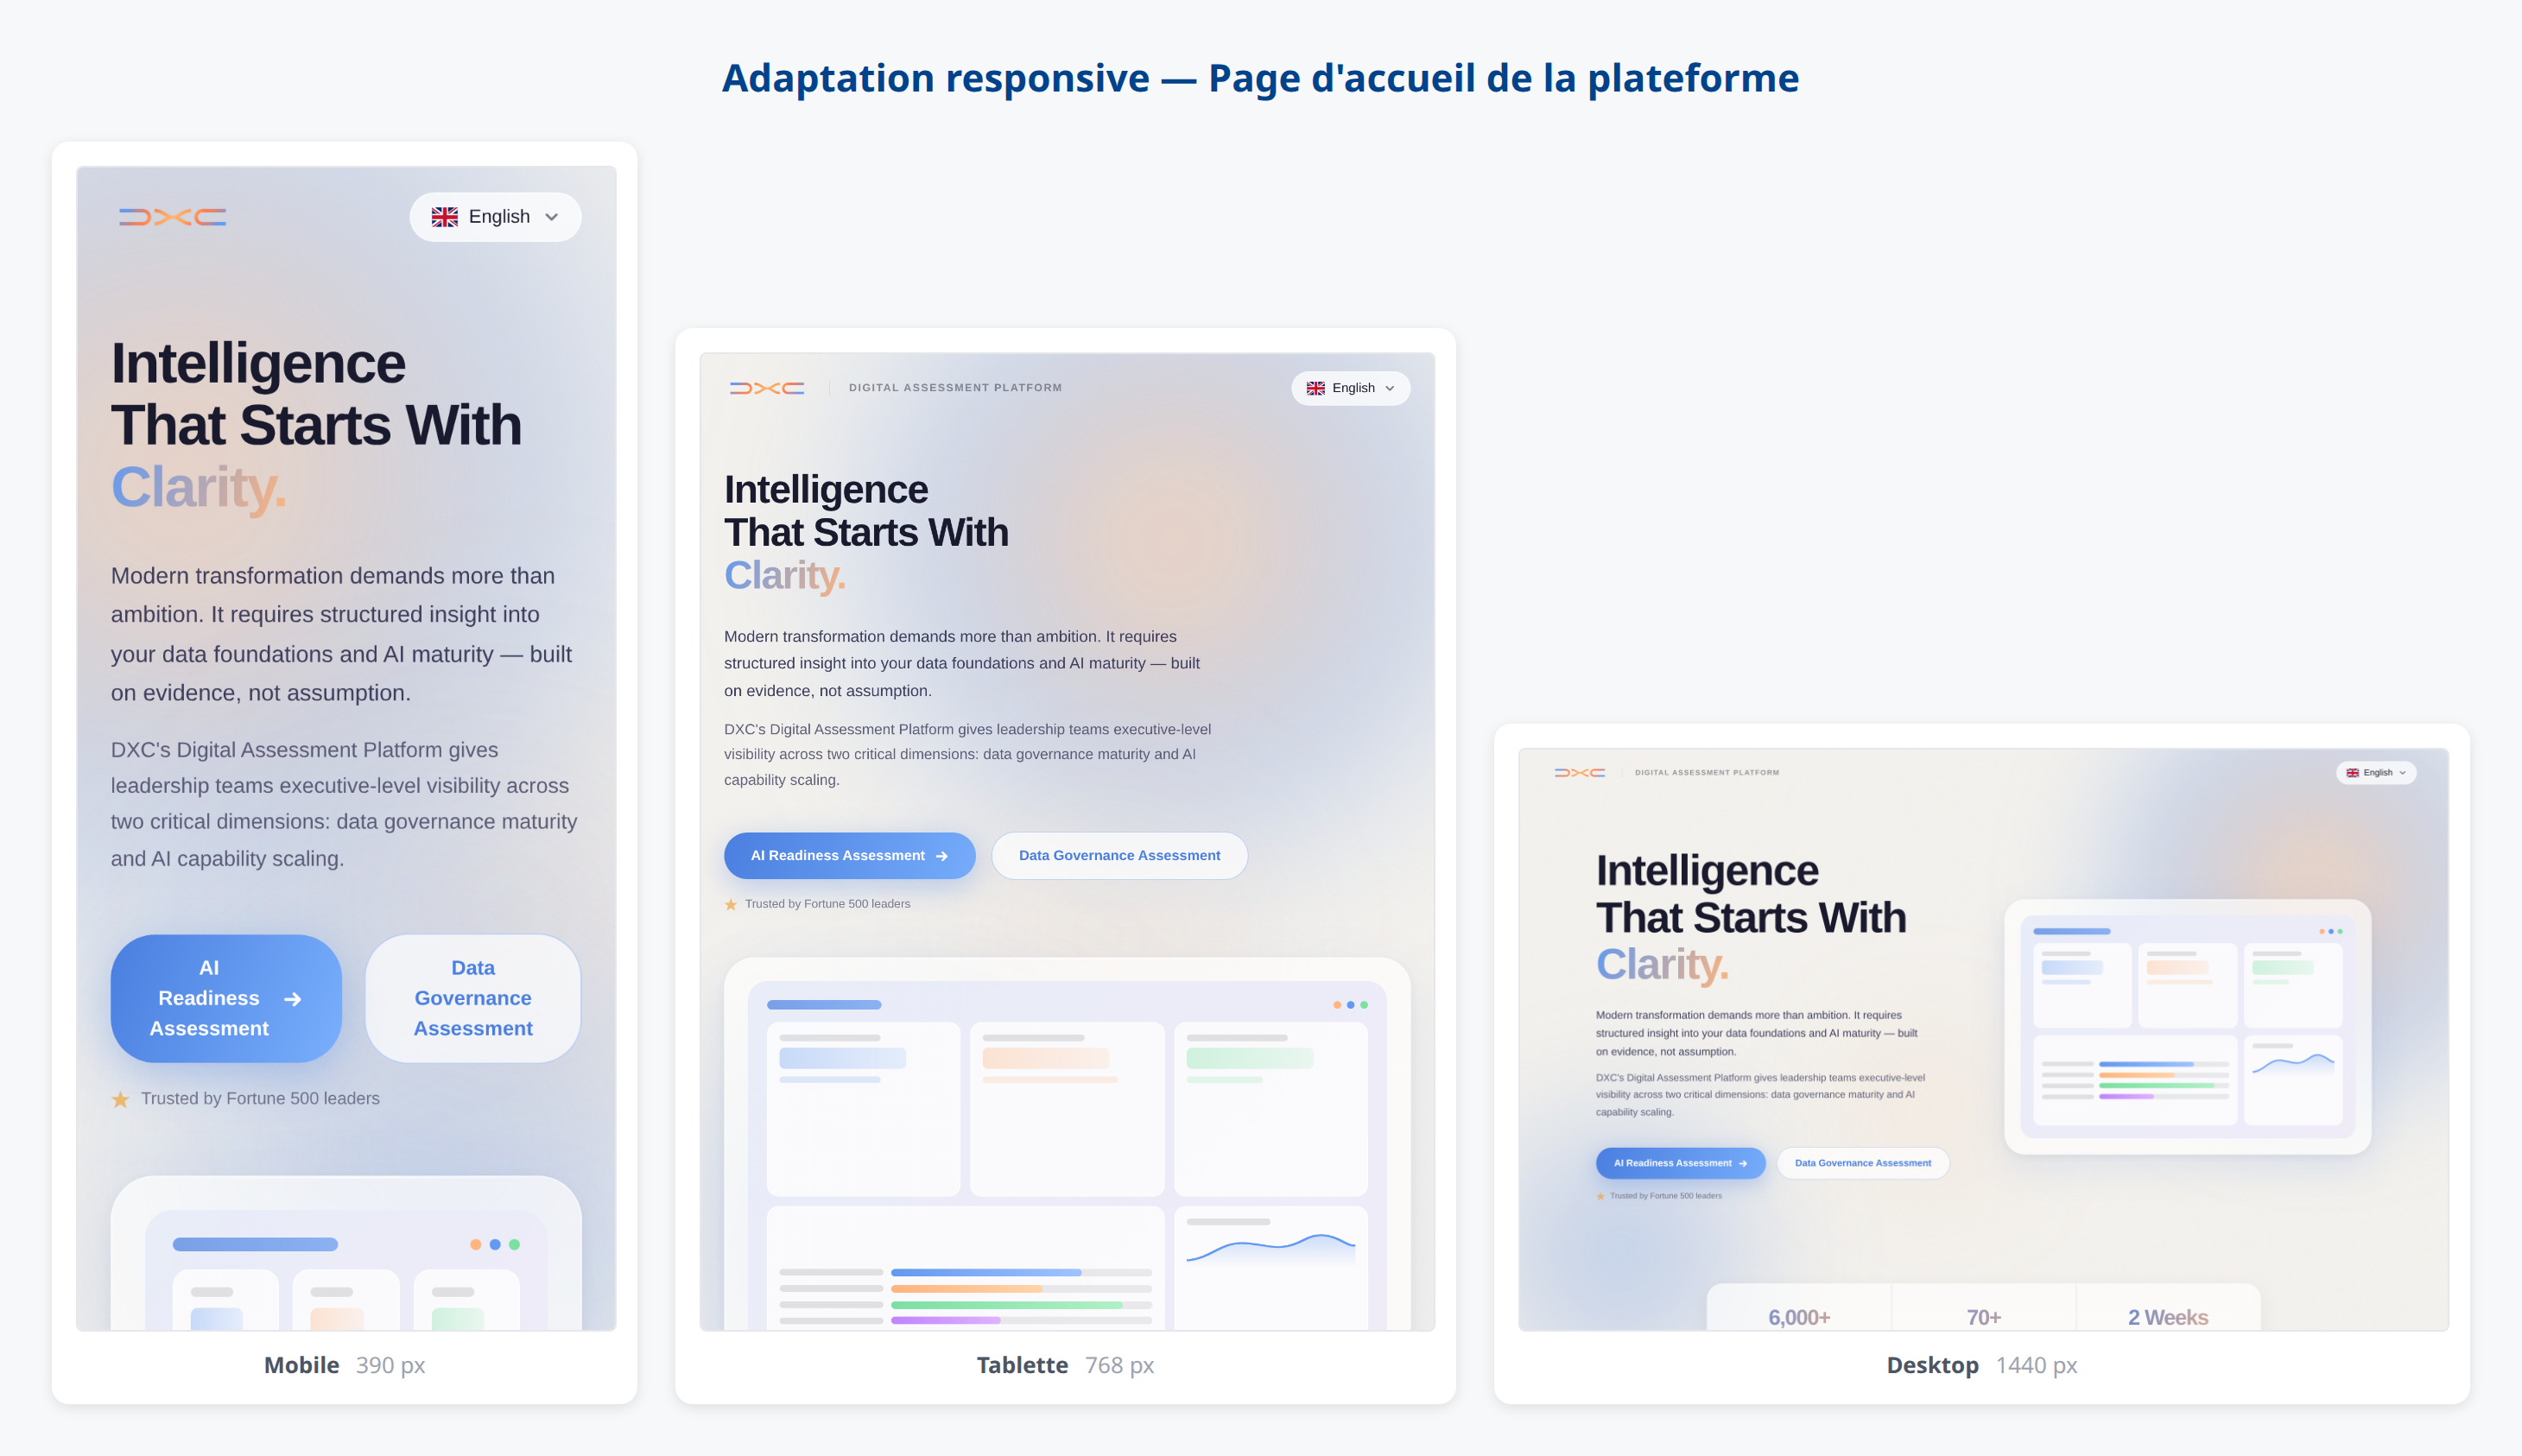
\includegraphics[width=0.95\textwidth]{figures/test-responsive.png}
\caption[Vérification responsive de la page d'accueil]{Comparaison côte à côte de la page d'accueil aux résolutions cibles mobile (390\,px), tablette (768\,px) et desktop (1440\,px). Le hero, les boutons d'accès aux évaluations et l'aperçu visuel s'adaptent en conservant la hiérarchie visuelle et la lisibilité du contenu.}
\label{fig:responsive}
\end{figure}

\begin{figure}[H]
\centering
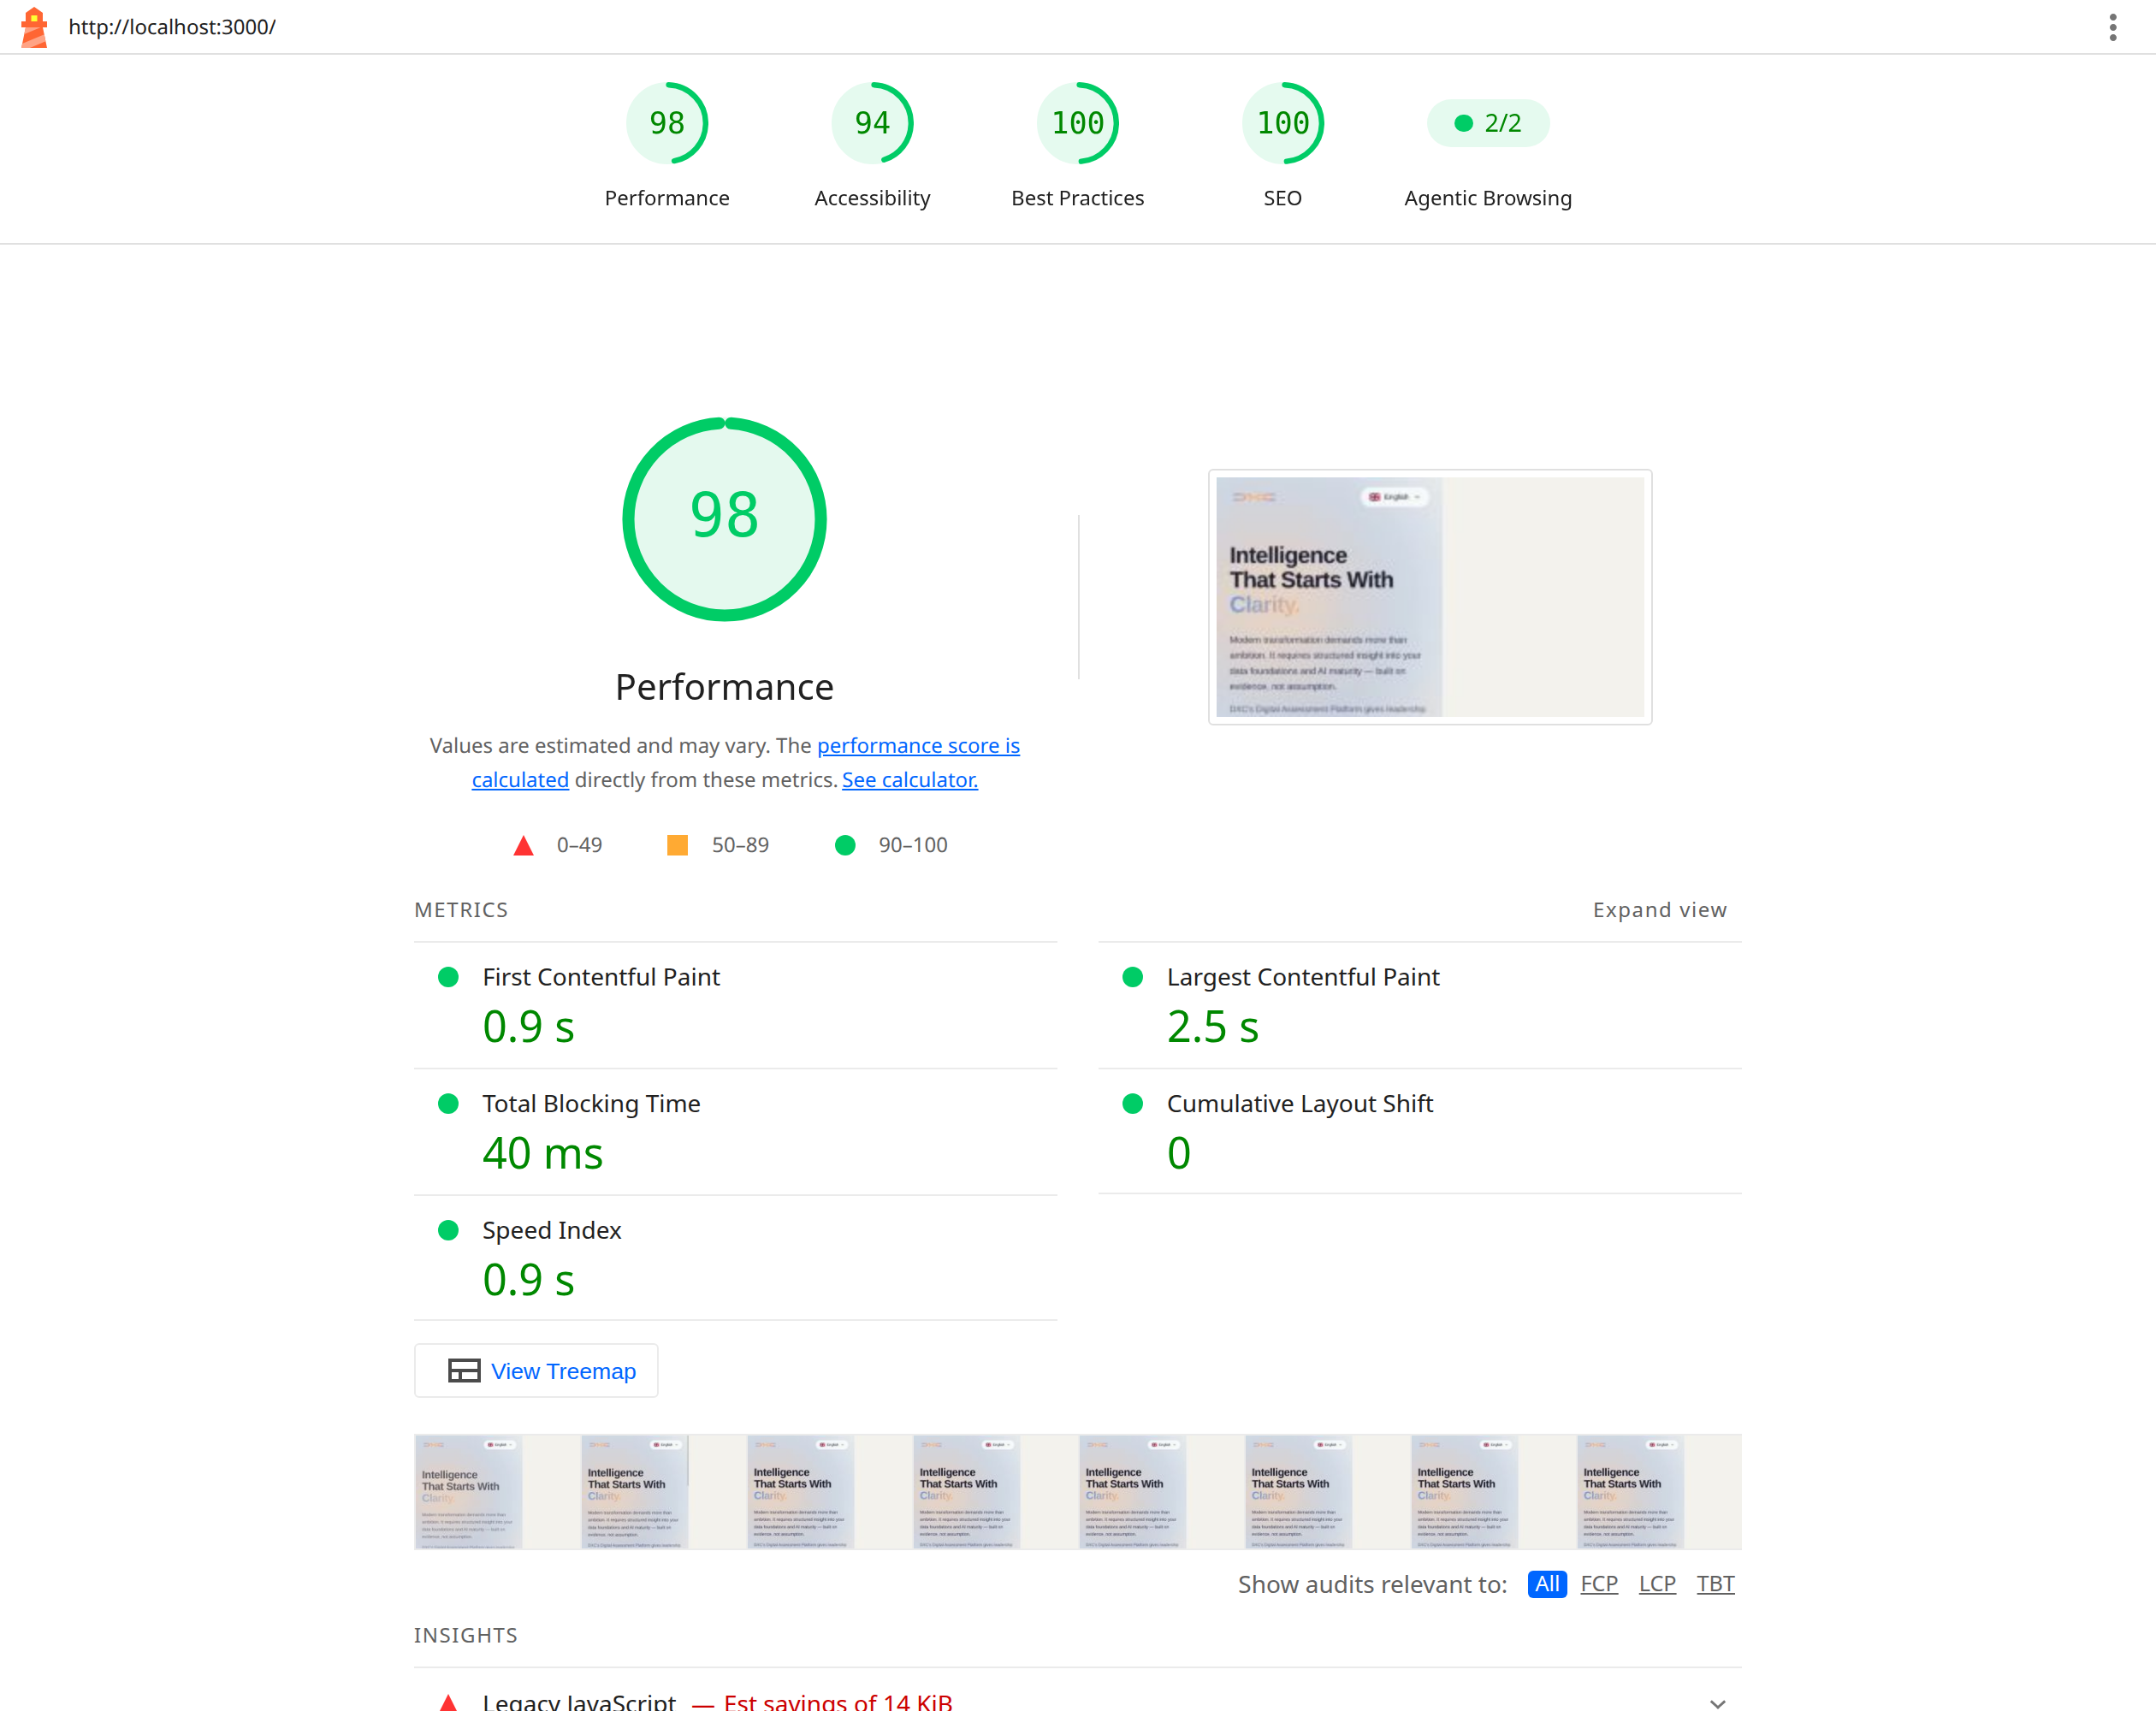
\includegraphics[width=0.92\textwidth]{figures/test-lighthouse.png}
\caption[Audit Lighthouse de la page d'accueil]{Audit Lighthouse de la page d'accueil exécuté en mode \textit{headless}~: 98 en performance (First Contentful Paint 0,9\,s, Largest Contentful Paint 2,5\,s, Cumulative Layout Shift nul), 94 en accessibilité, 100 en bonnes pratiques et 100 en SEO.}
\label{fig:lighthouse}
\end{figure}

\begin{table}[H]
\centering
\caption{Axes de validation appliqués à la plateforme.}
\begin{tabularx}{\textwidth}{>{\bfseries}L{4cm}Y}
\toprule
Axe de validation & Vérification réalisée \\
\midrule
Parcours client & Chargement du questionnaire, progression par section, changement de langue, soumission et confirmation. \\
Administration & Création, modification et consultation des sections, questions, choix, types d'évaluation et contenus multilingues. \\
Invitations & Création d'une invitation, copie du lien, suivi des statuts, prolongation de l'expiration et distinction interne/externe. \\
Analyse & Affichage des indicateurs, filtres, tableaux de soumissions, export CSV et ouverture du détail d'une réponse. \\
Sécurité & Vérification des routes protégées, du rôle administrateur et des accès aux services sensibles. \\
Interface & Contrôle responsive, lisibilité des tableaux, états vides, messages d'erreur et comportements de chargement. \\
\bottomrule
\end{tabularx}
\end{table}

\section*{Conclusion du chapitre}
Bout à bout, les quatre versions tracent la construction de la plateforme par couches successives~: la V1 a posé un socle fonctionnel autonome (parcours, administration, analytique, multilingue), la V2 y a intégré l'Agent IA dans les flux métier, la V3 a porté l'IA jusqu'au poste de l'administrateur et préparé le déploiement, et la V4 a consolidé la couverture multilingue de l'IA et l'édition des contenus générés. Les phases de stabilisation et d'industrialisation, moins visibles que l'ajout de fonctionnalités, ont eu autant d'importance dans la qualité finale du produit.
\setcounter{tocdepth}{2}

\chapter*{Conclusion générale et perspectives}
\markboth{Conclusion générale et perspectives}{}
\addcontentsline{toc}{chapter}{Conclusion générale et perspectives}
Ce projet de fin d'études a abouti à une plateforme web d'évaluation de la maturité Data Governance et AI Readiness, conçue pour répondre à un besoin clairement identifié chez DXC Technology~: remplacer un processus d'évaluation dispersé entre plusieurs supports par un environnement unique capable de gérer les questionnaires, les invitations, les soumissions, les résultats et les rapports. Les objectifs fixés en début de stage, rappelés dans l'introduction, ont été couverts par la solution livrée, qui prend en charge l'ensemble du cycle d'évaluation.

Côté technique, l'architecture multi-services adoptée (frontend Next.js, backend Spring Boot, base PostgreSQL, authentification Keycloak, service Agent IA en FastAPI) a permis d'isoler les responsabilités et de progresser par paliers vérifiables. Cette séparation a facilité l'intégration de l'Agent IA développé par Hiba Bouhnin, en limitant les zones d'adhérence entre couches et en autorisant des tests indépendants.

Ma contribution personnelle a porté sur la totalité de la plateforme applicative en dehors du module Agent IA : parcours d'évaluation multilingue avec prise en charge du RTL, espace administrateur et constructeur de questionnaires, gestion des invitations en modes interne et externe, services Spring Boot et persistance PostgreSQL, intégration Keycloak, tableau de bord analytique et raccordement côté interface des fonctions exposées par l'Agent IA. Le travail ne s'est pas limité à la réalisation des fonctionnalités~: il a aussi imposé de hiérarchiser des données complexes, de conserver des interfaces lisibles, de traiter les états d'erreur, de tenir compte des usages mobiles et d'assurer une communication maîtrisée entre les services.

Le projet a également mis en évidence l'importance des itérations de stabilisation. Les ajustements progressifs apportés aux tableaux de bord, à la sécurité des accès, au comportement responsive et à la traduction ont eu un effet direct sur la qualité perçue de la plateforme, parfois plus que l'ajout pur de fonctionnalités. Sur un plan personnel, ce stage m'a permis de consolider mes compétences en architecture full-stack, en gestion de projet agile et en collaboration sur un module développé en parallèle, dans un contexte professionnel exigeant.

\section*{Limites}
Le travail accompli appelle quelques limites. La plateforme livrée est une base fonctionnelle solide, mais elle gagnerait à être alimentée par un volume plus important de données réelles pour fiabiliser les comparaisons entre clients, domaines et secteurs. Les tableaux de bord fournissent déjà une lecture exploitable des résultats~; leur pertinence dépend toutefois de la qualité des réponses collectées et de la représentativité des questionnaires.

Les recommandations produites par l'Agent IA demandent une réserve similaire. Elles offrent un point de départ utile et un gain de temps pour le consultant, mais ne remplacent pas son expertise, surtout lorsque le contexte métier du client suppose une interprétation que l'algorithme ne peut deviner. La plateforme conserve donc, pour chaque rapport généré, le statut de brouillon soumis à validation humaine.

Enfin, un déploiement en production exigerait un travail complémentaire qui sort du périmètre de ce stage~: mise en place d'une supervision applicative, journalisation centralisée, stratégie de sauvegarde et de restauration de la base, gestion fine des droits d'accès au-delà de la simple distinction administrateur/consultant, et procédures de maintenance documentées.

\section*{Perspectives}
Plusieurs pistes pourraient prolonger ce travail. La plus directe serait d'accueillir de nouvelles familles d'évaluations (cybersécurité, cloud, conformité réglementaire) en tirant parti du référentiel configurable mis en place~; l'essentiel des écrans et services pourrait être réutilisé sans changement structurel.

Une deuxième piste consisterait à enrichir l'historique client, afin de suivre l'évolution de la maturité d'une organisation au fil de plusieurs campagnes successives. Cela permettrait de représenter la trajectoire d'un client dans le temps, plutôt que de raisonner à une seule date. Dans la continuité, des benchmarks anonymisés pourraient être construits pour situer un client par rapport à un ensemble de références, sans exposer de données sensibles.

La personnalisation des rapports est un troisième axe~: un \textit{workflow} de validation permettrait au consultant de contrôler, commenter et approuver les recommandations générées par l'Agent IA avant partage avec le client, en gardant trace des modifications. Enfin, un déploiement cloud avec observabilité, supervision et sauvegarde rapprocherait la solution d'un usage opérationnel à plus grande échelle.

\renewcommand{\bibname}{Références bibliographiques et webographiques}
\markboth{Références bibliographiques}{}
\bibliographystyle{IEEEtran}
\bibliography{references}

\appendix
\chapter{Annexes}

\section{Structure du dépôt source}
La plateforme est organisée en un \textit{monorepo} regroupant le frontend, le backend, le module d'Agent IA et la configuration des services partagés. Le listing~\ref{lst:structure} reproduit la hiérarchie effective du dépôt, telle qu'elle se présente sur la branche principale au moment de la livraison de la version V4.

\begin{figure}[H]
\centering
\begin{minipage}{0.92\textwidth}
\begin{verbatim}
ProjetPFE/
├── frontend/                  # Application Next.js 16 (TypeScript)
│   ├── app/                   # Pages : accueil, assessment, admin,
│   │   ├── admin/             #   analytics, ai-readiness, ...
│   │   ├── analytics/         # Tableau de bord analytique
│   │   ├── assessment/        # Parcours de réponse
│   │   ├── data-assessment/   # Variante Data Governance
│   │   ├── ai-readiness/      # Variante AI Readiness
│   │   ├── api/               # Routes API + proxy Agent IA
│   │   └── thank-you/         # Confirmation post-soumission
│   ├── components/            # Composants partagés
│   ├── context/               # LanguageContext, AuthContext, ...
│   ├── hooks/                 # Hooks React réutilisables
│   ├── lib/                   # api.ts, auth.ts, maturity.ts, ...
│   └── types/                 # Définitions TypeScript partagées
│
├── spring-backend/            # API Spring Boot 3.3 (Java 21)
│   └── src/main/java/com/dxc/assessment/
│       ├── DxcAssessmentApplication.java
│       ├── config/            # SecurityConfig, JacksonConfig, ...
│       ├── controller/        # Endpoints REST par domaine fonctionnel
│       ├── dto/               # Objets de transfert API
│       ├── exception/         # GlobalExceptionHandler
│       ├── model/             # Entités JPA (Section, Question, ...)
│       ├── repository/        # Spring Data JPA
│       ├── security/          # JwtAuthConverter, AuthScopeService
│       └── service/           # Services métier (logique applicative)
│
├── agent/                     # Module Agent IA (FastAPI / Python)
│   ├── main.py                # Endpoints REST IA et orchestration
│   └── prompts/               # Modèles de prompts par cas d'usage
│
├── keycloak/
│   └── realm-export.json      # Configuration du realm DXC
│
├── docker-compose.yml         # Orchestration des cinq services
├── init-schemas.sql           # Création des schémas PostgreSQL
└── Makefile                   # Commandes de développement courantes
\end{verbatim}
\end{minipage}
\refstepcounter{figure}\label{lst:structure}
\caption*{\textsc{Listing \thefigure}~: structure du dépôt source du projet.}
\end{figure}

\section{Cartographie des endpoints REST}
Le tableau~\ref{tab:endpoints} dresse la cartographie des principaux endpoints exposés par le backend Spring Boot. Pour chacun, sont précisés la méthode HTTP, le chemin, le rôle métier et le niveau d'authentification requis (\textit{public}, \textit{authentifié}, ou \textit{rôle administrateur}).

\begin{longtable}{>{\ttfamily\small}L{1.4cm} >{\ttfamily\small}L{5.8cm} L{5.0cm} >{\itshape\footnotesize}L{2.0cm}}
\caption{Cartographie des principaux endpoints REST de la plateforme.}
\label{tab:endpoints}\\
\toprule
\textbf{Méth.} & \textbf{Chemin} & \textbf{Rôle métier} & \textbf{Accès} \\
\midrule
\endfirsthead
\toprule
\textbf{Méth.} & \textbf{Chemin} & \textbf{Rôle métier} & \textbf{Accès} \\
\midrule
\endhead
GET    & /assessments/\{type\}              & Structure d'une évaluation               & public \\
POST   & /submissions                        & Création d'une soumission                & public \\
GET    & /submissions/\{id\}                 & Détail d'une soumission                  & consultant \\
GET    & /invitations                        & Liste des invitations                    & consultant \\
POST   & /invitations                        & Création d'une invitation                & consultant \\
POST   & /invitations/bulk                   & Création en masse                        & consultant \\
PATCH  & /invitations/\{id\}/expiry          & Prolongation d'expiration                & consultant \\
POST   & /invitations/\{id\}/resend          & Relance par courriel                     & consultant \\
GET    & /invitations/validate/\{token\}     & Vérification d'un lien d'invitation      & public \\
DELETE & /invitations/\{id\}                 & Suppression d'une invitation             & consultant \\
GET    & /analytics                          & Données agrégées (vue overview)          & consultant \\
GET    & /analytics/heatmap                  & Carte de chaleur par domaine             & consultant \\
GET    & /analytics/client-overview          & Vue d'un client                          & consultant \\
GET    & /analytics/client-drilldown         & Drilldown soumission                     & consultant \\
GET    & /domains                            & Liste des domaines clients               & consultant \\
POST   & /domains                            & Création d'un domaine                    & admin \\
POST   & /admin/sections                     & Création d'une section                   & admin \\
PUT    & /admin/sections/\{id\}              & Modification d'une section               & admin \\
POST   & /admin/sections/\{sid\}/questions   & Ajout d'une question                     & admin \\
PUT    & /admin/questions/\{id\}             & Modification d'une question              & admin \\
POST   & /admin/questions/\{qid\}/choices    & Ajout d'un choix                         & admin \\
GET    & /api/assessment-types               & Liste des types d'évaluation             & public \\
POST   & /api/assessment-types               & Création d'un type d'évaluation          & admin \\
POST   & /api/assessment-types/\{key\}/logo  & Téléversement d'un logo                  & admin \\
POST   & /reports/\{submissionId\}/send      & Envoi du rapport au client               & consultant \\
GET    & /auth/by-email                      & Recherche d'un utilisateur               & admin \\
GET    & /health                             & Sonde de santé applicative               & public \\
\bottomrule
\end{longtable}

\section{Schéma relationnel principal}
La figure~\ref{fig:erd} reproduit le schéma entité-relation de la base PostgreSQL tel qu'il est mis en place par Spring Data JPA. Les attributs textuels multilingues (titres, descriptions, libellés, choix) sont stockés sous forme \texttt{JSONB} (par exemple \texttt{\{"en": ..., "fr": ..., "ar": ...\}}), ce qui permet d'ajouter une langue sans modification du schéma. La table~\ref{tab:schema} reprend les colonnes principales pour référence rapide.

\begin{figure}[p]
\centering
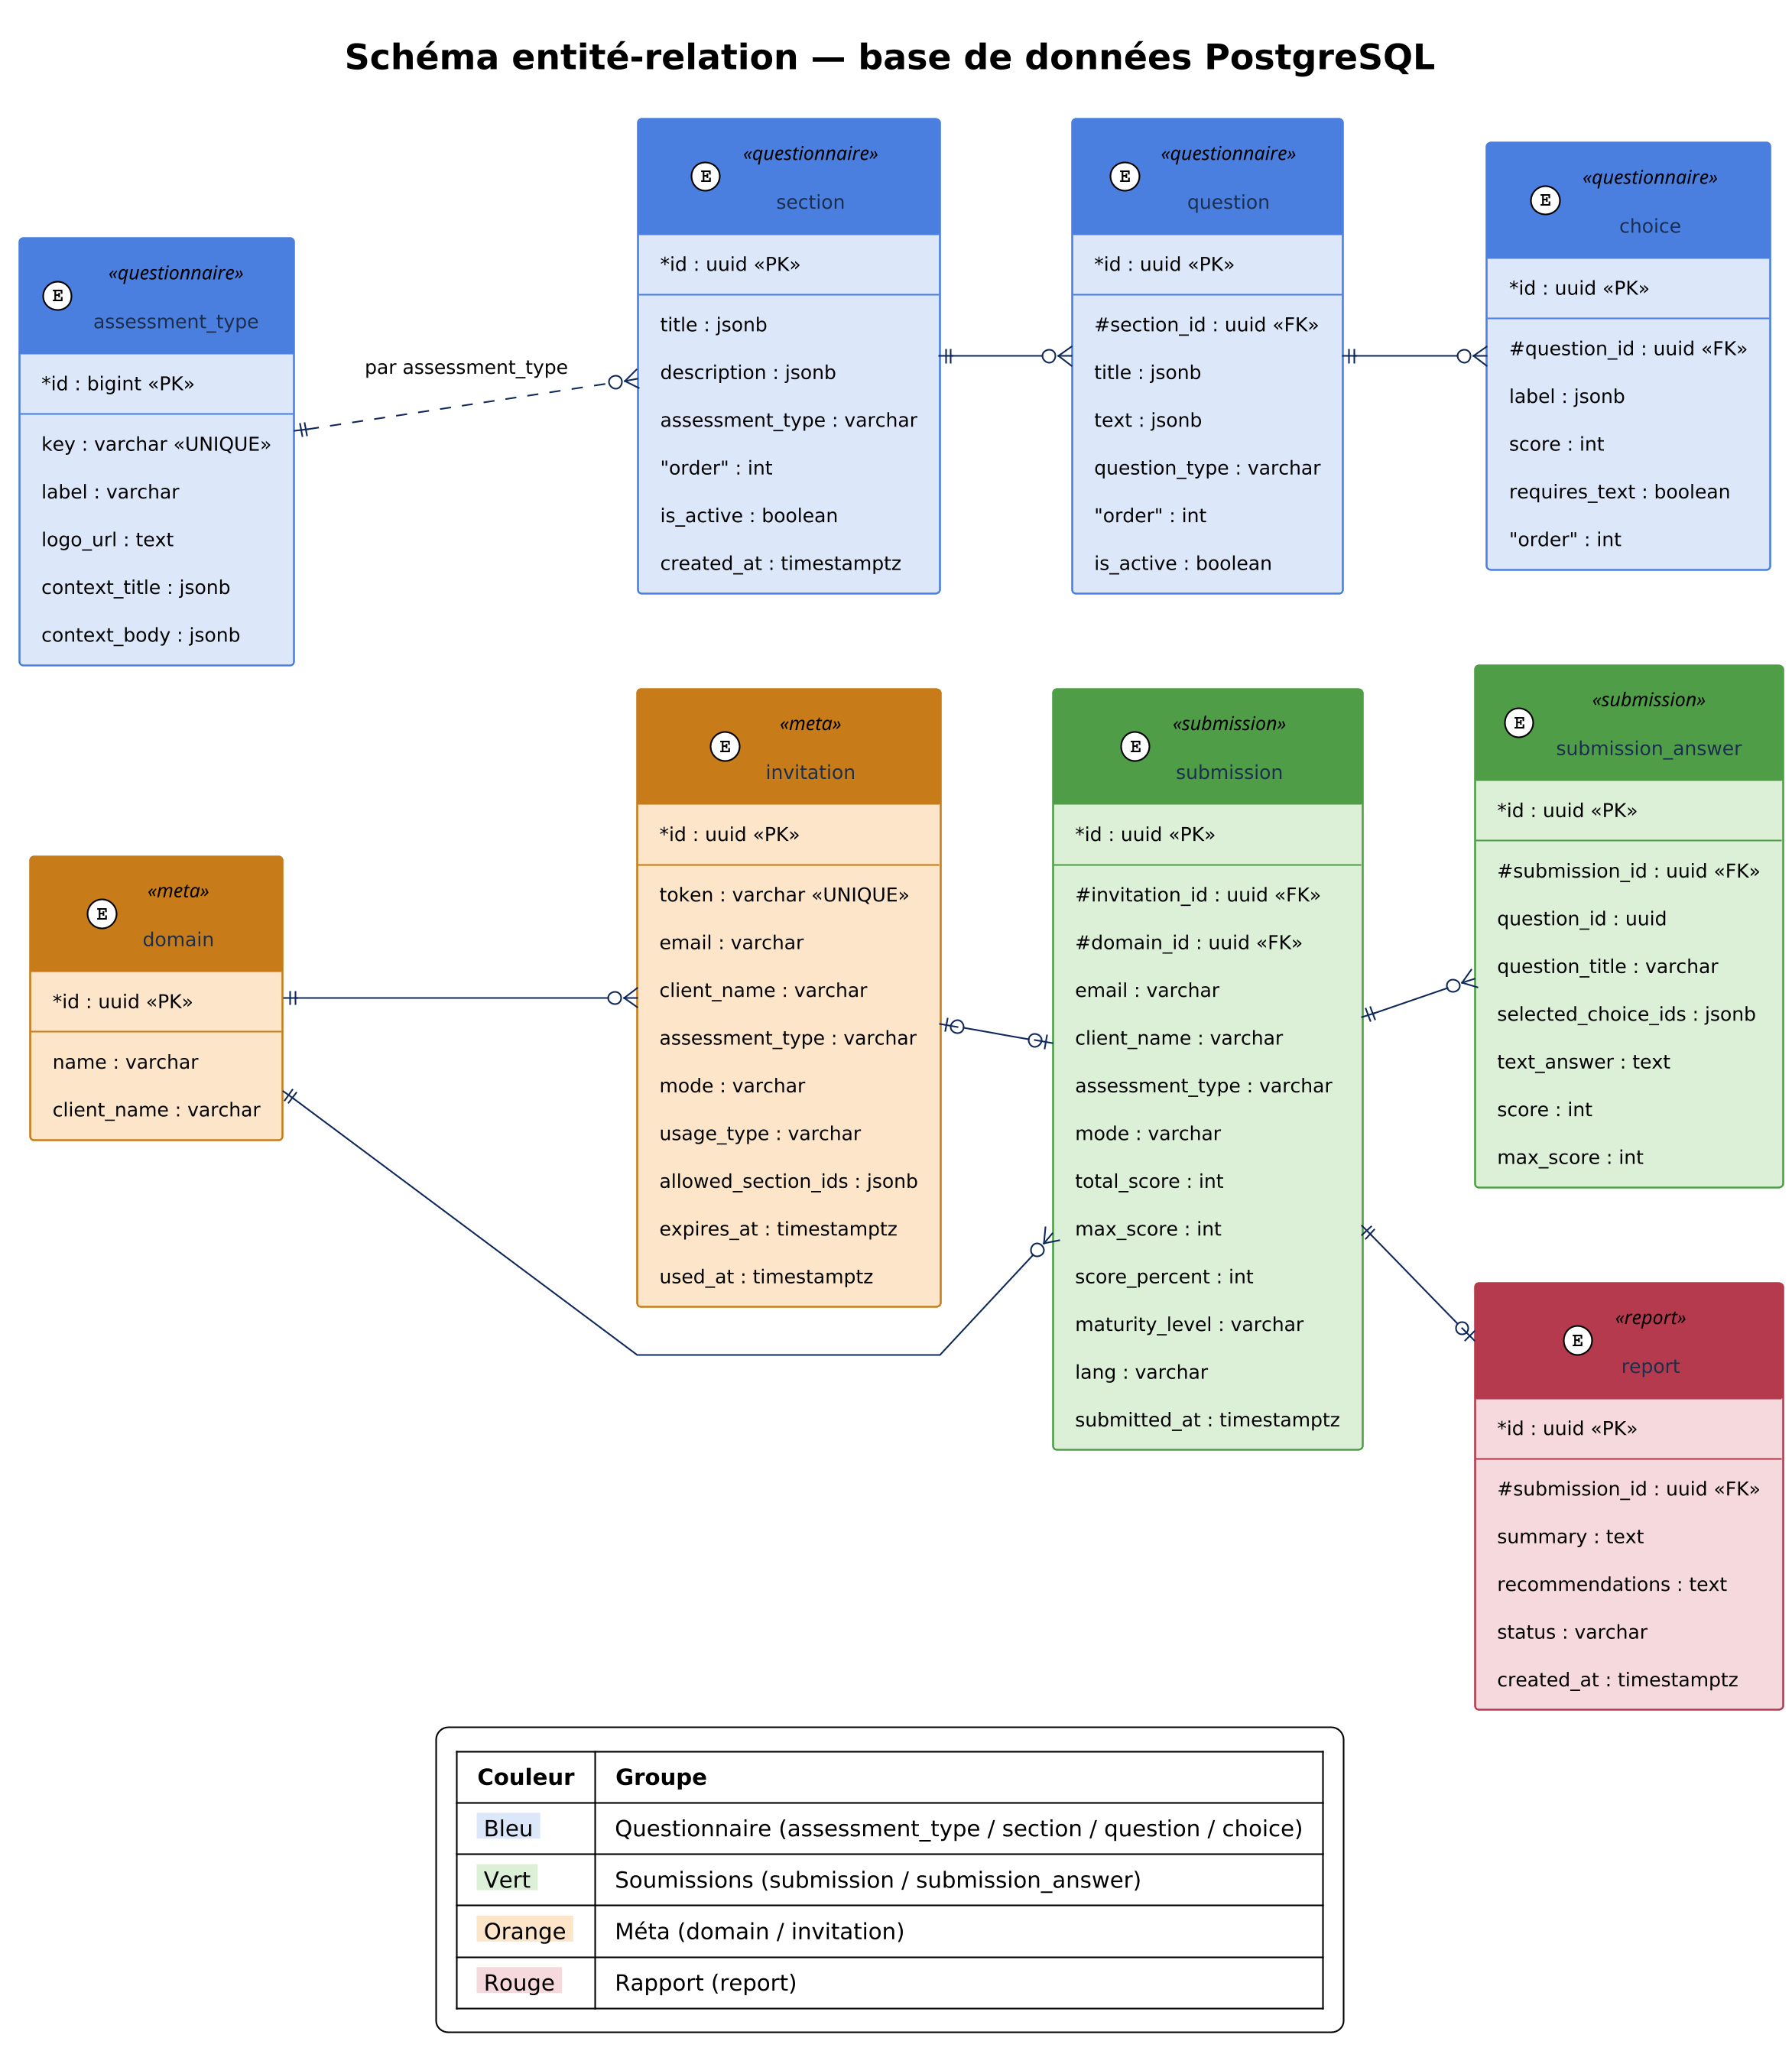
\includegraphics[width=\textwidth, height=0.85\textheight, keepaspectratio]{figures/uml-erd.png}
\caption[Schéma entité-relation PostgreSQL]{Schéma entité-relation des principales tables PostgreSQL de la plateforme. Les clés primaires (\texttt{PK}) et étrangères (\texttt{FK}) sont signalées sur chaque colonne~; les attributs multilingues sont typés \texttt{jsonb}. Le code couleur reprend les groupes du diagramme de classes~: questionnaire (bleu), soumissions (vert), méta (orange) et rapport (rouge).}
\label{fig:erd}
\end{figure}

\begin{longtable}{>{\bfseries}L{3.0cm} L{4.0cm} L{6.0cm}}
\caption{Colonnes principales des entités persistées dans la base PostgreSQL.}
\label{tab:schema}\\
\toprule
Table & Colonne & Description \\
\midrule
\endfirsthead
\toprule
Table & Colonne & Description \\
\midrule
\endhead
assessment\_type & code, name, logo\_url & Type d'évaluation (Data Gov., AI Readiness, ...) \\
section & id, title (JSONB), order\_index, assessment\_type\_id & Section d'un questionnaire \\
question & id, text (JSONB), question\_type, section\_id & Question rattachée à une section \\
choice & id, label (JSONB), score, question\_id & Choix de réponse scoré \\
domain & id, name, description & Domaine métier du client \\
invitation & id, token, status, expires\_at, domain\_id, allowed\_section\_ids (JSONB) & Lien d'invitation, à usage unique \\
submission & id, score, language, domain\_id, invitation\_id & Soumission d'une évaluation \\
submission\_answer & id, value, score, submission\_id, question\_id & Réponse individuelle à une question \\
report & id, format, generated\_at, submission\_id & Rapport associé à une soumission \\
\bottomrule
\end{longtable}

\section{Extrait de la configuration Docker Compose}
Le listing~\ref{lst:compose} reproduit un extrait du fichier \texttt{docker-compose.yml} montrant la déclaration des services PostgreSQL et Keycloak, leur \textit{healthcheck} et leur partage du volume de schémas d'initialisation.

\begin{figure}[H]
\centering
\begin{minipage}{0.95\textwidth}
\begin{verbatim}
services:
  db:
    image: postgres:16-alpine
    container_name: dxc_db
    environment:
      POSTGRES_USER: ${POSTGRES_USER:-dxc}
      POSTGRES_PASSWORD: ${POSTGRES_PASSWORD:-dxc_secret}
      POSTGRES_DB: ${POSTGRES_DB:-dxc_assessment}
    volumes:
      - postgres_data:/var/lib/postgresql/data
      - ./init-schemas.sql:/docker-entrypoint-initdb.d/init-schemas.sql:ro
    healthcheck:
      test: ["CMD-SHELL", "pg_isready -U dxc -d dxc_assessment"]
      interval: 10s
      retries: 15

  keycloak:
    image: quay.io/keycloak/keycloak:26.6.2
    container_name: dxc_keycloak
    command: start-dev --import-realm
    environment:
      KC_DB: postgres
      KC_DB_URL: jdbc:postgresql://db:5432/dxc_assessment
      KC_DB_SCHEMA: keycloak
    ports:
      - "8080:8080"
    volumes:
      - ./keycloak/realm-export.json:/opt/keycloak/data/import/realm-export.json:ro
    depends_on:
      db: { condition: service_healthy }
\end{verbatim}
\end{minipage}
\refstepcounter{figure}\label{lst:compose}
\caption*{\textsc{Listing \thefigure}~: extrait de \texttt{docker-compose.yml}~--- services PostgreSQL et Keycloak.}
\end{figure}

\section{Pipeline d'intégration continue}
Le listing~\ref{lst:ci} reproduit la structure des quatre jobs GitHub Actions exécutés sur chaque \textit{push} et \textit{pull request} ciblant la branche \texttt{main} (les directives \texttt{uses:} d'\textit{actions} standard sont omises par souci de concision).

\begin{figure}[H]
\centering
\begin{minipage}{0.95\textwidth}
\small
\begin{verbatim}
name: CI
on:
  push:         { branches: [main] }
  pull_request: { branches: [main] }

jobs:
  frontend:           # Node 22, cache npm
    steps:
      - npm ci --ignore-scripts
      - npx tsc --noEmit
      - npm run test:analytics
      - npm run lint
      - npm run format:check

  backend:            # Java 21 (Temurin), cache Maven
    steps:
      - mvn -q verify

  agent:              # Python 3.12
    steps:
      - pip install -r agent/requirements.txt -r agent/requirements-dev.txt
      - ruff check agent/
      - ruff format --check agent/
      - pytest agent/

  docker-build:       # smoke test des images Docker
    steps:
      - docker build -t dxc-backend  ./spring-backend
      - docker build -t dxc-agent    ./agent
      - docker build -t dxc-frontend ./frontend
\end{verbatim}
\end{minipage}
\refstepcounter{figure}\label{lst:ci}
\caption*{\textsc{Listing \thefigure}~: structure du fichier \texttt{.github/workflows/ci.yml}.}
\end{figure}

\section{Échelle de maturité et calcul du score}
Le score de maturité d'une soumission est calculé en agrégeant les points obtenus sur l'ensemble des réponses, rapportés au score maximum théorique. Le résultat est exprimé en pourcentage entier, puis converti en un niveau qualitatif à l'aide des seuils définis dans le tableau~\ref{tab:maturity-scale}. Cette échelle à quatre niveaux est partagée entre le backend (méthode \texttt{maturityLevel} de \texttt{SubmissionService}) et le frontend (utilitaire \texttt{maturity.ts}) afin d'éviter toute divergence entre l'affichage et le scoring.

\begin{table}[H]
\centering
\caption{Échelle de maturité utilisée pour qualifier le score d'une évaluation.}
\label{tab:maturity-scale}
\begin{tabularx}{\textwidth}{>{\bfseries}L{3.0cm}L{2.0cm}Y}
\toprule
Niveau & Seuil & Interprétation \\
\midrule
Initial    & $<$ 30\,\%    & Pratiques informelles, peu structurées, fortement dépendantes des individus. \\
Emerging   & 30 -- 54\,\%  & Premières démarches structurantes en place, mais hétérogènes selon les domaines. \\
Developing & 55 -- 79\,\%  & Cadre méthodologique généralisé, processus mesurés et améliorés régulièrement. \\
Advanced   & $\geq$ 80\,\% & Capacité reconnue, optimisée en continu et alignée avec les standards du secteur. \\
\bottomrule
\end{tabularx}
\end{table}

\begin{figure}[H]
\centering
\begin{minipage}{0.85\textwidth}
\begin{verbatim}
int scorePercent = maxScore > 0
        ? Math.round((totalScore * 100.0f) / maxScore)
        : 0;

private String maturityLevel(int scorePercent) {
    if (scorePercent >= 80) return "Advanced";
    if (scorePercent >= 55) return "Developing";
    if (scorePercent >= 30) return "Emerging";
    return "Initial";
}
\end{verbatim}
\end{minipage}
\refstepcounter{figure}\label{lst:maturity}
\caption*{\textsc{Listing \thefigure}~: calcul du pourcentage et conversion en niveau de maturité (\texttt{SubmissionService.java}).}
\end{figure}

\section{Consommation atomique des invitations}
Le lien d'invitation est à usage unique~: dès qu'un client soumet ses réponses, l'invitation doit être marquée comme consommée pour empêcher toute soumission ultérieure avec le même jeton. Pour éviter une condition de concurrence en cas de double-clic ou de tentative malveillante, le marquage n'est pas géré par une lecture puis une écriture en deux temps, mais par une seule requête \texttt{UPDATE} conditionnelle, exécutée sous contrainte de transaction. Si la requête modifie une ligne, l'invitation était bien valide et est désormais consommée~; si elle n'en modifie aucune, c'est qu'elle était déjà utilisée, expirée ou révoquée, et la soumission est refusée.

\begin{figure}[H]
\centering
\begin{minipage}{0.95\textwidth}
\begin{verbatim}
@Modifying
@Query("UPDATE Invitation i SET i.usedAt = :now " +
       "WHERE i.token = :token " +
       "  AND i.usedAt IS NULL " +
       "  AND (i.expiresAt IS NULL OR i.expiresAt > :now)")
int markUsedAtomically(@Param("token") String token,
                       @Param("now")   Instant now);
\end{verbatim}
\end{minipage}
\refstepcounter{figure}\label{lst:invitation-atomic}
\caption*{\textsc{Listing \thefigure}~: requête JPQL atomique de consommation d'invitation (\texttt{InvitationRepository.java}).}
\end{figure}

\section{Configuration du reverse proxy Caddy en production}
En production sur Azure, l'entrée HTTPS publique est assurée par un reverse proxy \textbf{Caddy} qui démultiplexe les requêtes vers les trois services exposés. Caddy obtient automatiquement les certificats TLS auprès de Let's Encrypt via le protocole ACME, en utilisant l'adresse e-mail fournie en variable d'environnement. Les noms d'hôte et l'adresse de notification ACME sont externalisés par variables Compose, ce qui rend la configuration identique entre les environnements de tests et de production.

\begin{figure}[H]
\centering
\begin{minipage}{0.85\textwidth}
\begin{verbatim}
{
    email {$ACME_EMAIL}
}

{$PUBLIC_HOSTNAME} {
    encode zstd gzip
    header Strict-Transport-Security "max-age=0"

    # Keycloak — flux d'authentification
    handle /auth* {
        reverse_proxy keycloak:8080
    }

    # Backend Spring Boot — API métier (préfixe /svc retiré)
    handle_path /svc/* {
        reverse_proxy backend:8000
    }

    # Frontend Next.js — par défaut
    handle {
        reverse_proxy frontend:3000
    }
}
\end{verbatim}
\end{minipage}
\refstepcounter{figure}\label{lst:caddy}
\caption*{\textsc{Listing \thefigure}~: \texttt{caddy/Caddyfile}~--- démultiplexage HTTPS de la plateforme en production.}
\end{figure}

\section{Mapping des rôles Keycloak vers Spring Security}
Le backend extrait les rôles applicatifs depuis la claim \texttt{realm\_access.roles} du jeton JWT signé par Keycloak, puis les convertit en \texttt{GrantedAuthority} préfixés \texttt{ROLE\_} afin de pouvoir être utilisés directement par les annotations Spring Security et la chaîne de filtres. Cette conversion est encapsulée dans un \texttt{JwtAuthenticationConverter} dédié, déclaré dans la configuration de sécurité. Les routes publiques (parcours d'évaluation, soumission, validation d'invitation, sondes de santé) sont explicitement autorisées sans authentification, le reste exige le rôle \texttt{EXPERT} ou \texttt{ADMIN}.

\begin{figure}[H]
\centering
\begin{minipage}{0.95\textwidth}
\begin{verbatim}
.authorizeHttpRequests(auth -> auth
    .requestMatchers(HttpMethod.GET,  "/health").permitAll()
    .requestMatchers(HttpMethod.GET,  "/assessments/**").permitAll()
    .requestMatchers(HttpMethod.POST, "/submissions").permitAll()
    .requestMatchers(HttpMethod.GET,  "/invitations/validate/**").permitAll()
    .requestMatchers(HttpMethod.GET,  "/api/assessment-types").permitAll()
    .anyRequest().hasAnyRole("ADMIN", "EXPERT")
)
.oauth2ResourceServer(oauth2 -> oauth2
    .jwt(jwt -> jwt.jwtAuthenticationConverter(jwtAuthenticationConverter()))
);

private Converter<Jwt, Collection<GrantedAuthority>> keycloakRealmRoleConverter() {
    return jwt -> {
        Map<String, Object> realmAccess = jwt.getClaimAsMap("realm_access");
        if (realmAccess == null || !realmAccess.containsKey("roles")) {
            return Collections.emptyList();
        }
        @SuppressWarnings("unchecked")
        List<String> roles = (List<String>) realmAccess.get("roles");
        return roles.stream()
            .map(role -> new SimpleGrantedAuthority("ROLE_" + role))
            .collect(Collectors.toList());
    };
}
\end{verbatim}
\end{minipage}
\refstepcounter{figure}\label{lst:security}
\caption*{\textsc{Listing \thefigure}~: extrait de \texttt{SecurityConfig.java}~--- règles d'accès et conversion des rôles Keycloak en autorités Spring.}
\end{figure}

\section{Contenus multilingues~: stockage JSONB et helper \texttt{localize()}}
Les titres, descriptions et libellés affichés à l'utilisateur sont stockés sous forme de colonnes \texttt{JSONB} contenant une carte de langue vers traduction. Cette représentation évite la duplication des entités par langue, permet d'ajouter une langue sans modifier le schéma et conserve la cohérence entre la version originale et ses traductions au sein d'une même ligne. Côté backend, ces colonnes sont typées \texttt{Map<String, String>} dans les entités JPA. Côté frontend, un helper \texttt{localize()} centralise la résolution de la langue active avec un repli sur l'anglais puis sur la première valeur disponible.

\begin{figure}[H]
\centering
\begin{minipage}{0.95\textwidth}
\begin{verbatim}
// Exemple : section "Data Quality Management" stockée en JSONB
{
  "en": "Data Quality Management",
  "fr": "Gestion de la qualité des données",
  "ar": "إدارة جودة البيانات"
}

// Backend : entité JPA Section.java
@Column(nullable = false, columnDefinition = "jsonb")
private Map<String, String> title;

@Column(columnDefinition = "jsonb")
private Map<String, String> description;

// Frontend : helper de résolution multilingue (lib/api.ts)
export type I18nText = Record<string, string>;

export function localize(map: I18nText | null | undefined,
                         lang: string): string {
  if (!map) return "";
  return map[lang] || map["en"] || Object.values(map)[0] || "";
}
\end{verbatim}
\end{minipage}
\refstepcounter{figure}\label{lst:i18n}
\caption*{\textsc{Listing \thefigure}~: structure d'un attribut multilingue côté base, côté entité JPA et côté frontend.}
\end{figure}

\section{Échelle visuelle de maturité côté frontend}
Pour garantir la cohérence entre le scoring backend et l'affichage des résultats dans le tableau de bord analytique, les seuils de l'échelle de maturité sont partagés via un utilitaire dédié côté frontend (\texttt{lib/maturity.ts}). Ce module expose, pour chaque pourcentage de score, une couleur de texte et une couleur d'arrière-plan, utilisées par les cartes d'indicateurs, les badges et les tableaux d'évolution.

\begin{figure}[H]
\centering
\begin{minipage}{0.85\textwidth}
\begin{verbatim}
// frontend/lib/maturity.ts
export function scoreColor(pct: number): string {
  if (pct >= 80) return "#22a06b";  // Advanced (vert)
  if (pct >= 55) return "#4A7FE0";  // Developing (bleu)
  if (pct >= 30) return "#e8711a";  // Emerging (orange)
  return "#e34935";                  // Initial (rouge)
}

export function scoreBg(pct: number, a = 1): string {
  if (pct >= 80) return `rgba(34,160,107,${a})`;
  if (pct >= 55) return `rgba(74,127,224,${a})`;
  if (pct >= 30) return `rgba(232,113,26,${a})`;
  return `rgba(227,73,53,${a})`;
}
\end{verbatim}
\end{minipage}
\refstepcounter{figure}\label{lst:scorecolor}
\caption*{\textsc{Listing \thefigure}~: harmonisation des seuils backend et frontend via \texttt{maturity.ts}.}
\end{figure}

\section{Glossaire métier}
\begin{longtable}{>{\bfseries}L{4.0cm} L{10.0cm}}
\caption{Glossaire des termes métier utilisés dans le rapport.}\\
\toprule
Terme & Définition \\
\midrule
\endfirsthead
\toprule
Terme & Définition \\
\midrule
\endhead
Data Governance & Ensemble des pratiques, règles et outils encadrant la qualité, la sécurité et le cycle de vie des données d'une organisation. \\
AI Readiness & Évaluation du niveau de préparation d'une organisation à concevoir et exploiter des solutions d'intelligence artificielle de façon fiable. \\
Évaluation de maturité & Démarche structurée visant à situer une organisation sur une échelle de maturité, généralement par axe ou par domaine. \\
Référentiel & Ensemble structuré des sections, questions, choix de réponse et scores qui définit le contenu d'une évaluation. \\
Soumission & Réponse complète d'un répondant à une évaluation, comprenant l'ensemble des choix retenus et la langue utilisée. \\
Invitation & Lien sécurisé à usage unique permettant à un client de répondre à une évaluation sans création de compte. \\
Mode interne / externe & Distinction entre une évaluation menée par un consultant pour le compte d'un client et une évaluation remplie par le client lui-même. \\
Agent IA & Service indépendant exposant les fonctions de génération de rapports, de recommandations et d'assistance conversationnelle. \\
Score de maturité & Valeur calculée à partir des choix de réponse, exprimée sur une échelle continue ou en niveaux qualitatifs. \\
Heatmap & Représentation graphique sous forme de grille colorée, utilisée dans le tableau de bord pour visualiser rapidement les scores faibles ou élevés par client et par section. \\
Monorepo & Organisation du code source dans laquelle plusieurs applications ou modules (frontend, backend, agent) cohabitent dans un même dépôt Git, partageant outillage et conventions. \\
Reverse proxy & Service en frontal réseau qui reçoit les requêtes HTTPS publiques et les redirige vers les composants internes appropriés (frontend, backend, Keycloak) en gérant terminaison TLS et certificats. \\
JSONB & Type de colonne PostgreSQL stockant du JSON sous forme binaire indexable, utilisé pour les champs multilingues (titre, description) et les listes d'identifiants. \\
SSO Keycloak & Authentification unique fédérée par Keycloak comme fournisseur d'identité, autorisant un accès consultant/administrateur via OAuth 2.0 et OpenID Connect. \\
PKCE & Extension d'OAuth 2.0 protégeant les clients publics contre l'interception du \textit{code d'autorisation}, requise par Auth.js côté Next.js. \\
RTL & \textit{Right-To-Left}~: sens d'écriture appliqué à l'arabe, qui implique une inversion de la direction de lecture et de la mise en page. \\
\bottomrule
\end{longtable}

\end{document}
